\documentclass[twocolumn]{../../common/aa}
%\documentclass[referee]{aa}

\usepackage{graphicx}
\usepackage{amsmath,amsfonts,amssymb}
\usepackage[varg]{txfonts}
\usepackage{color}
\usepackage{natbib}
\usepackage{float}
%\usepackage{stfloats}
\usepackage{dblfloatfix}
\usepackage{afterpage}
\usepackage{ifthen}
\usepackage[morefloats=12]{morefloats}
\usepackage{placeins}
\usepackage{multicol}
\usepackage{multirow}
\bibpunct{(}{)}{;}{a}{}{,}
\usepackage[switch]{lineno}
\definecolor{linkcolor}{rgb}{0.6,0,0}
\definecolor{citecolor}{rgb}{0,0,0.75}
\definecolor{urlcolor}{rgb}{0.12,0.46,0.7}
\usepackage[breaklinks, colorlinks, urlcolor=urlcolor,
    linkcolor=linkcolor,citecolor=citecolor,pdfencoding=auto]{hyperref}
\hypersetup{linktocpage}
\usepackage{bold-extra}
\usepackage{xcolor}
\newcommand{\gray}[0]{\color{gray}}

\usepackage{lipsum}

%\usepackage[grid,
%  gridcolor=red!20,
%  subgridcolor=green!20,
%  gridunit=cm]{eso-pic}


%Planck style file, to be used with A&A style to produce Planck papers for publication.
%
% version 28 September 2010 --- useful macros --- CRL
% version 17 October 2010   --- first cut at important instrument values, from Daniele Mennella and
%                               Francois Bouchet, 13 October 2010 --- CRL
% version 18 October 2010   --- LFI FWHM changed to one value per feed, rather than M & S separately
%                               LFI FWHM uncertainties added for individual feeds.  Corrections made
%                               to LFI values. --- Andrea Zacchei
% version 24 October 2010   --- added to and corrected definitions.  No changes made to instrument
%                               quantities. --- CRL 
% version 31 October 2010   --- added definition of \muKHz. --- CRL
%
% version 15 November 2010  --- fixed conflict with aa.cls in definition of \endtable
%                               by naming the command below "\endPlancktable".  See section
%                               13.16 of the Style Guide.
%
% version 06 December 2010  --- Set up names with and without units.
%                               Add \allearlypapers command to ensure that all early papers are
%                               included in the reference list.
%                               Define macro for the name of the 4He JT cooler.
%
% version 07 December 2010  --- removed extraneous "planck2011-1.2" entry in \allearlypapers
%
% version 12 December 2010  --- added \endPlancktablewide command to set tablenotes to the full
%                               page width in the \begin{table*}...\end{table*} environment when
%                               the ``twocolumn'' option is specified in the \documentclass command.
%                               (It would be more elegant to extract the appropriate width from the
%                               aa.cls system at the time of execution, but that is buried more
%                               deeply in the system than I investigated.)
%
% version 05 January 2011   --- added unit \MJysr.  HFI performance values updated per FRB email
%                               01/05/2011 02:38-0800, and Brendan Crill email 01/05/2011 18:08 -0800.
%
% version 06 January 2011   --- changed \scriptscriptstyle primes to \scriptstyle, to better match the
%                               tx fonts used by A&A.
%
% version 07 January 2011   --- modified \allearlypapers to correspond with final early paper list.  
%                               Fixed 545 GHz center frequency.
%
% version 07 January 2011b  --- changed LFI white-noise sensitivity numbers to correct problem with units
%
% version 05 July 2011      --- added \Msol and \Lsol to get the symbols for solar mass and luminosity.
%                               Deleted previous definitions of \solar and \sol, which were equivalent
%                               to the new \Msol.
%
% version 16 August 2011    --- changed comments on \endPlancktable and \endPlancktablewide for clarity
%
% version 11 September 2011 --- changed definition of \tablenote to make footnote labels italic, as per A\&A
%
% version 26 April 2011     --- changed definition of \Planck to agree with what is said in the Style Guide (!)
%
% version 04 Dec 2013       --- included 2013 results references
%
% version 17 Jan 2014       --- included fix to bibtex file v4.3, i.e. \providecommand{\sorthelp}[1]{}
%
% version 26 Jul 2014       --- fixed incompatibility problem with aa.cls v8.0 and v8.2.  v8.2 should now be used
%                               for all Planck papers.
%                           --- fixed problem in definition of "\all2013resultspapers" that introduced a blanck
%                               into the reference to p06b.
%                           --- removed all the parameter definition stuff at the end.  We weren't using it, and
%                               it took up a lot of space.
%
% version 28 Jan 2015       --- added "\alltwentyfiftennresultspapers" and corrected "\all2013resultspapers" to
%                               "\all20thirteenresultspapers",
%
% Usage:  after the \documentclass[traditabstract]{aa} command in the La\TeX\ input file,
%         add this command:      \input Planck.tex


\def\setsymbol#1#2{\expandafter\def\csname #1\endcsname{#2}}
\def\getsymbol#1{\csname #1\endcsname}

%-----------------------------------------------------------------------
% Planck
%-----------------------------------------------------------------------
\def\Planck{\textit{Planck}}

%-----------------------------------------------------------------------
% The Planck Helium-4 JT cooler
%-----------------------------------------------------------------------
\def\HeJT{$^4$He-JT}

%-----------------------------------------------------------------------
% To include all Planck Early Results papers in the reference lists
%-----------------------------------------------------------------------
\def\allearlypapers{\nocite{planck2011-1.1, planck2011-1.3, planck2011-1.4, planck2011-1.5, planck2011-1.6, planck2011-1.7, planck2011-1.10, planck2011-1.10sup, planck2011-5.1a, planck2011-5.1b, planck2011-5.2a, planck2011-5.2b, planck2011-5.2c, planck2011-6.1, planck2011-6.2, planck2011-6.3a, planck2011-6.4a, planck2011-6.4b, planck2011-6.6, planck2011-7.0, planck2011-7.2, planck2011-7.3, planck2011-7.7a, planck2011-7.7b, planck2011-7.12, planck2011-7.13}}

%-----------------------------------------------------------------------
% To include all Planck 2013 Results papers in the reference lists
%-----------------------------------------------------------------------
\def\alltwentythirteenresultspapers{\nocite{planck2013-p01, planck2013-p02, planck2013-p02a, planck2013-p02d, planck2013-p02b, planck2013-p03, planck2013-p03c, planck2013-p03f, planck2013-p03d, planck2013-p03e, planck2013-p01a, planck2013-p06, planck2013-p03a, planck2013-pip88, planck2013-p08, planck2013-p11, planck2013-p12, planck2013-p13, planck2013-p14, planck2013-p15, planck2013-p05b, planck2013-p17, planck2013-p09, planck2013-p09a, planck2013-p20, planck2013-p19, planck2013-pipaberration, planck2013-p05, planck2013-p05a, planck2013-pip56, planck2013-p06b, planck2013-p01a}}

%-----------------------------------------------------------------------
% To include all Planck 2015 Results papers in the reference lists
%-----------------------------------------------------------------------
\def\alltwentyfifteenresultspapers{\nocite{planck2014-a01, planck2014-a03, planck2014-a04, planck2014-a05, planck2014-a06, planck2014-a07, planck2014-a08, planck2014-a09, planck2014-a11, planck2014-a12, planck2014-a13, planck2014-a14, planck2014-a15, planck2014-a16, planck2014-a17, planck2014-a18, planck2014-a19, planck2014-a20, planck2014-a22, planck2014-a24, planck2014-a26, planck2014-a28, planck2014-a29, planck2014-a30, planck2014-a31, planck2014-a35, planck2014-a36, planck2014-a37, planck2014-ES}}

%-----------------------------------------------------------------------
% Tables
%-----------------------------------------------------------------------
\newbox\tablebox    \newdimen\tablewidth
\def\leaderfil{\leaders\hbox to 5pt{\hss.\hss}\hfil}
%
% use the following definition of \endPlancktable for ApJ style notes to tables, set to the 
%         width of the table
% \def\endPlancktable{\tablewidth=\wd\tablebox 
%
% use the following definitions of \endPlancktable and \endPlancktablewide for A&A style notes 
% set to one-column  or full-page width, respectively
\def\endPlancktable{\tablewidth=\columnwidth 
    $$\hss\copy\tablebox\hss$$
    \vskip-\lastskip\vskip -2pt}
\def\endPlancktablewide{\tablewidth=\textwidth 
    $$\hss\copy\tablebox\hss$$
    \vskip-\lastskip\vskip -2pt}
\def\tablenote#1 #2\par{\begingroup \parindent=0.8em
    \abovedisplayshortskip=0pt\belowdisplayshortskip=0pt
    \noindent
    $$\hss\vbox{\hsize\tablewidth \hangindent=\parindent \hangafter=1 \noindent
    \hbox to \parindent{$^#1$\hss}\strut#2\strut\par}\hss$$
    \endgroup}
\def\doubleline{\vskip 3pt\hrule \vskip 1.5pt \hrule \vskip 5pt}

%-----------------------------------------------------------------------
% useful macros
%-----------------------------------------------------------------------
%
\def\L2{\ifmmode L_2\else $L_2$\fi}
%
\def\dtt{\Delta T/T}
\def\DeltaT{\ifmmode \Delta T\else $\Delta T$\fi}
\def\deltat{\ifmmode \Delta t\else $\Delta t$\fi}
\def\fknee{\ifmmode f_{\rm knee}\else $f_{\rm knee}$\fi}
\def\Fmax{\ifmmode F_{\rm max}\else $F_{\rm max}$\fi}
%
\def\solar{\ifmmode{\rm M}_{\mathord\odot}\else${\rm M}_{\mathord\odot}$\fi}
\def\Msolar{\ifmmode{\rm M}_{\mathord\odot}\else${\rm M}_{\mathord\odot}$\fi}
\def\Lsolar{\ifmmode{\rm L}_{\mathord\odot}\else${\rm L}_{\mathord\odot}$\fi}
%
\def\inv{\ifmmode^{-1}\else$^{-1}$\fi}
\def\mo{\ifmmode^{-1}\else$^{-1}$\fi}
\def\sup#1{\ifmmode ^{\rm #1}\else $^{\rm #1}$\fi}
\def\expo#1{\ifmmode \times 10^{#1}\else $\times 10^{#1}$\fi}
%
\def\,{\thinspace}
\def\lsim{\mathrel{\raise .4ex\hbox{\rlap{$<$}\lower 1.2ex\hbox{$\sim$}}}}
\def\gsim{\mathrel{\raise .4ex\hbox{\rlap{$>$}\lower 1.2ex\hbox{$\sim$}}}}
\let\lea=\lsim
\let\gea=\gsim
\def\simprop{\mathrel{\raise .4ex\hbox{\rlap{$\propto$}\lower 1.2ex\hbox{$\sim$}}}}
%
\def\deg{\ifmmode^\circ\else$^\circ$\fi}
\def\pdeg{\ifmmode $\setbox0=\hbox{$^{\circ}$}\rlap{\hskip.11\wd0 .}$^{\circ}
          \else \setbox0=\hbox{$^{\circ}$}\rlap{\hskip.11\wd0 .}$^{\circ}$\fi}
\def\arcs{\ifmmode {^{\scriptstyle\prime\prime}}
          \else $^{\scriptstyle\prime\prime}$\fi}
\def\arcm{\ifmmode {^{\scriptstyle\prime}}
          \else $^{\scriptstyle\prime}$\fi}
\newdimen\sa  \newdimen\sb
\def\parcs{\sa=.07em \sb=.03em
     \ifmmode \hbox{\rlap{.}}^{\scriptstyle\prime\kern -\sb\prime}\hbox{\kern -\sa}
     \else \rlap{.}$^{\scriptstyle\prime\kern -\sb\prime}$\kern -\sa\fi}
\def\parcm{\sa=.08em \sb=.03em
     \ifmmode \hbox{\rlap{.}\kern\sa}^{\scriptstyle\prime}\hbox{\kern-\sb}
     \else \rlap{.}\kern\sa$^{\scriptstyle\prime}$\kern-\sb\fi}
%
\def\ra[#1 #2 #3.#4]{#1\sup{h}#2\sup{m}#3\sup{s}\llap.#4}
\def\dec[#1 #2 #3.#4]{#1\deg#2\arcm#3\arcs\llap.#4}
\def\deco[#1 #2 #3]{#1\deg#2\arcm#3\arcs}
\def\rra[#1 #2]{#1\sup{h}#2\sup{m}}
%
\def\page{\vfill\eject}
\def\dots{\relax\ifmmode \ldots\else $\ldots$\fi}
%
%-----------------------------------------------------------------------
% units
%-----------------------------------------------------------------------
%
\def\WHzsr{\ifmmode $W\,Hz\mo\,sr\mo$\else W\,Hz\mo\,sr\mo\fi}
\def\mHz{\ifmmode $\,mHz$\else \,mHz\fi}
\def\GHz{\ifmmode $\,GHz$\else \,GHz\fi}
\def\mKs{\ifmmode $\,mK\,s$^{1/2}\else \,mK\,s$^{1/2}$\fi}
\def\muKs{\ifmmode \,\mu$K\,s$^{1/2}\else \,$\mu$K\,s$^{1/2}$\fi}
\def\muKRJs{\ifmmode \,\mu$K$_{\rm RJ}$\,s$^{1/2}\else \,$\mu$K$_{\rm RJ}$\,s$^{1/2}$\fi}
\def\muKHz{\ifmmode \,\mu$K\,Hz$^{-1/2}\else \,$\mu$K\,Hz$^{-1/2}$\fi}
\def\MJysr{\ifmmode \,$MJy\,sr\mo$\else \,MJy\,sr\mo\fi}
\def\MJysrmK{\ifmmode \,$MJy\,sr\mo$\,mK$_{\rm CMB}\mo\else \,MJy\,sr\mo\,mK$_{\rm CMB}\mo$\fi}
\def\microns{\ifmmode \,\mu$m$\else \,$\mu$m\fi}
\def\micron{\microns}
\def\muK{\ifmmode \,\mu$K$\else \,$\mu$\hbox{K}\fi}
\def\microK{\ifmmode \,\mu$K$\else \,$\mu$\hbox{K}\fi}
\def\muW{\ifmmode \,\mu$W$\else \,$\mu$\hbox{W}\fi}
\def\kms{\ifmmode $\,km\,s$^{-1}\else \,km\,s$^{-1}$\fi}
\def\kmsMpc{\ifmmode $\,\kms\,Mpc\mo$\else \,\kms\,Mpc\mo\fi}
%
%
%----------------------------------------------------------------------
% set up machinery to list Planck papers in roman numeral order.
%----------------------------------------------------------------------

\providecommand{\sorthelp}[1]{}


\def\WMAP{\emph{WMAP}}
\def\WMAPnine{\emph{WMAP9}}
\def\COBE{\emph{COBE}}
\def\wmap{\emph{WMAP}}
\def\planck{\emph{Planck}}
\def\Planck{\emph{Planck}}
\def\LCDM{$\Lambda$CDM}
\def\ffp{FFP6}
\def\unionmask{U73}
\def\nside{N_{\mathrm{side}}}

\def\healpix{\texttt{HEALPix}}
\def\commander{\texttt{Commander}}
\def\commanderone{\texttt{Commander1}}
\def\commandertwo{\texttt{Commander2}}
\def\commanderthree{\texttt{Commander3}}
\def\ruler{\texttt{Ruler}}
\def\comrul{\texttt{Commander-Ruler}}
\def\CR{\texttt{C-R}}
\def\nilc{\texttt{NILC}}
\def\gnilc{\texttt{GNILC}}
\def\sevem{\texttt{SEVEM}}
\def\smica{\texttt{SMICA}}
\def\CamSpec{\texttt{CamSpec}}
\def\Plik{\texttt{Plik}}
\def\XFaster{\texttt{XFaster}}
\def\sroll2{\texttt{SRoll2}}

\newcommand{\phm}{\phantom{-}}
\renewcommand{\d}[0]{\vec{d}}
\renewcommand{\t}[0]{\vec{t}}
\newcommand{\A}[0]{\mathrm{A}}
\newcommand{\B}[0]{\mathrm{B}}
\newcommand{\Y}[0]{\tens{Y}}
\newcommand{\n}[0]{\vec{n}}
\newcommand{\red}[0]{\color{red}}
\newcommand{\green}[0]{\color{green}}
\newcommand{\s}[0]{\vec{s}}
\renewcommand{\a}[0]{\vec{a}}
\newcommand{\m}[0]{\vec{m}}
\newcommand{\f}[0]{\vec{f}}
\newcommand{\F}[0]{\tens{F}}
\newcommand{\T}[0]{\tens{T}}
\newcommand{\Cp}[0]{\tens{C}}
\renewcommand{\L}[0]{\tens{L}}
\newcommand{\g}[0]{\vec{g}}
\newcommand{\N}[0]{\tens{N}}
\newcommand{\M}[0]{\tens{M}}
\newcommand{\iN}[0]{\tens{N}^{-1}}
\newcommand{\iM}[0]{\tens{M}^{-1}}
\newcommand{\w}[0]{\vec{w}}
\renewcommand{\S}[0]{\tens{S}}
\renewcommand{\r}[0]{\vec{r}}
\renewcommand{\u}[0]{\vec{u}}
\newcommand{\q}[0]{\vec{q}}
\renewcommand{\v}[0]{\vec{v}}
\renewcommand{\P}[0]{\tens{P}}
\newcommand{\dt}[0]{d_t}
\newcommand{\di}[0]{d_i}
\newcommand{\nt}[0]{n_t}
\newcommand{\st}[0]{s_t}
\newcommand{\mt}[0]{m_t}
\newcommand{\ft}[0]{f_t}
\newcommand{\Te}[0]{T_{\rm e}}
\newcommand{\EM}[0]{\rm EM}
\newcommand{\mathsc}[1]{{\normalfont\textsc{#1}}}
\newcommand{\hi}{\ensuremath{\mathsc {Hi}}}
\newcommand{\bpbold}{\bfseries{\scshape{BeyondPlanck}}}
\newcommand{\BP}{\textsc{BeyondPlanck}}
\newcommand{\bp}{\textsc{BeyondPlanck}}
\newcommand{\cosmoglobe}{\textsc{Cosmoglobe}}
\newcommand{\Cosmoglobe}{\textsc{Cosmoglobe}}
\newcommand{\lfi}[0]{LFI}
\newcommand{\hfi}[0]{HFI}
\newcommand{\npipe}[0]{\texttt{NPIPE}}
\newcommand{\K}[0]{\textit K}
\newcommand{\Ka}[0]{\textit{Ka}}
\newcommand{\Q}[0]{\textit Q}
\newcommand{\V}[0]{\textit V}
\newcommand{\W}[0]{\textit W}
\newcommand{\e}{\mathrm e}
\newcommand{\cvar}{\ensuremath{c(\vartheta, \varphi, \psi)}}


\def\Tcmb{\ifmmode T_\mathrm{CMB}\else $T_{\mathrm{CMB}}$\fi}
\def\Tdust{\ifmmode T_\mathrm{d}\else $T_{\mathrm{d}}$\fi}
\def\scmb{\ifmmode s_\mathrm{CMB}\else $s_{\mathrm{CMB}}$\fi}
\def\squad{\ifmmode s_\mathrm{quad}\else $s_{\mathrm{quad}}$\fi}
\def\ssynch{\ifmmode s_\mathrm{s}\else $s_\mathrm{s}$\fi}
\def\sdust{\ifmmode s_\mathrm{d}\else $s_{\mathrm{d}}$\fi}
\def\ssdust{\ifmmode s_\mathrm{sd}\else $s_{\mathrm{sd}}$\fi}
\def\same{\ifmmode s_\mathrm{ame}\else $s_{\mathrm{ame}}$\fi}
\def\ssrc{\ifmmode s_\mathrm{src}\else $s_{\mathrm{src}}$\fi}
\def\sco{\ifmmode s_\mathrm{CO}\else $s_{\mathrm{CO}}$\fi}
\def\sff{\ifmmode s_\mathrm{ff}\else $s_{\mathrm{ff}}$\fi}
\def\gff{\ifmmode g_\mathrm{ff}\else $g_{\mathrm{ff}}$\fi}
\def\fsynch{\ifmmode f_\mathrm{s}\else $f_{\mathrm{s}}$\fi}
\def\fsd{\ifmmode f_\mathrm{sd}\else $f_{\mathrm{sd}}$\fi}
\def\fame{\ifmmode f_\mathrm{ame}\else $f_{\mathrm{ame}}$\fi}
\def\alphasrc{\ifmmode \alpha_\mathrm{src}\else $\alpha_{\mathrm{src}}$\fi}
\def\bdust{\ifmmode \beta_\mathrm{d}\else $\beta_{\mathrm{d}}$\fi}
\def\bsynch{\ifmmode \beta_\mathrm{s}\else $\beta_{\mathrm{s}}$\fi} 
\def\bsun{\ifmmode \beta_\mathrm{sun}\else $\beta_{\mathrm{sun}}$\fi} 
\def\nuzeros{\ifmmode \nu_{0,\mathrm{s}}\else $\nu_{0,\mathrm{s}}$\fi} 
\def\nuzeroff{\ifmmode \nu_{0,\mathrm{ff}}\else $\nu_{0,\mathrm{ff}}$\fi} 
\def\nuzerod{\ifmmode \nu_{0,\mathrm{d}}\else $\nu_{0,\mathrm{d}}$\fi} 
\def\nuzeroame{\ifmmode \nu_{0,\mathrm{ame}}\else $\nu_{0,\mathrm{ame}}$\fi} 
\def\nuzerosd{\ifmmode \nu_{0,\mathrm{}}\else $\nu_{0,\mathrm{sd}}$\fi} 
\def\nuzerosrc{\ifmmode \nu_{0,\mathrm{src}}\else $\nu_{0,\mathrm{src}}$\fi} 
\def\nup{\ifmmode \nu_{\mathrm{p}}\else $\nu_{\mathrm{p}}$\fi} 
\def\alphasd{\ifmmode \alpha_{\mathrm{sd}}\else $\alpha_{\mathrm{sd}}$\fi} 
\def\Te{\ifmmode T_{\mathrm{e}}\else $T_{\mathrm{e}}$\fi} 
\def\kB{\ifmmode k_\mathrm{B}\else $k_{\mathrm{B}}$\fi} 



\usepackage[T1]{fontenc}


\def\bC{\tens{C}}
\def\ba{\vec{a}}
\def\ncha{N_\mathrm{cha}}
\def\nfg{N_\mathrm{fg}}

\newcommand{\ncorr}{\vec n_\mathrm{corr}}
\newcommand{\Dbp}{\Delta_\mathrm{bp}}

%\modulolinenumbers[5]
%\linenumbers

\newcommand{\includegraphicsdpi}[3]{
    \pdfimageresolution=#1  % Change the dpi of images
    \includegraphics[#2]{#3}
    \pdfimageresolution=72  % Change it back to the default
}

\renewcommand{\topfraction}{1.0}	% max fraction of floats at top
    \renewcommand{\bottomfraction}{1.0}	% max fraction of floats at bottom
    %   Parameters for TEXT pages (not float pages):
    \setcounter{topnumber}{2}
    \setcounter{bottomnumber}{2}
    \setcounter{totalnumber}{4}     % 2 may work better
    \setcounter{dbltopnumber}{2}    % for 2-column pages
    \renewcommand{\dbltopfraction}{0.9}	% fit big float above 2-col. text
    \renewcommand{\textfraction}{0.04}	% allow minimal text w. figs
    %   Parameters for FLOAT pages (not text pages):
    \renewcommand{\floatpagefraction}{0.9}	% require fuller float pages
	% N.B.: floatpagefraction MUST be less than topfraction !!
    \renewcommand{\dblfloatpagefraction}{0.9}	% require fuller float pages

\def\adj{^{\dagger}}
\def\tp{^{\rm T}}
\def\inv{^{-1}}
\def\lm{{\ell m}}

\begin{document}

\title{\bfseries{\Cosmoglobe\ I. Improved \emph{Wilkinson Microwave Anisotropy Probe} frequency maps through Bayesian end-to-end analysis}}
%This author list corresponds to \title{Author list for L04\_CMB\_Foregrounds\_Extraction}
%Prepared by M. Lopez-Caniego (Marcos.Lopez.Caniego@sciops.esa.int), ESAC/ESA
%This version is from Thu Jul 12 18:11:48 2018 CET
%\subtitle{There are 152 co-authors in this list}
\newcommand{\oslo}[0]{1}
\newcommand{\iiabangalore}[0]{2}

\author{\small
D.~J.~Watts\inst{\ref{uio}}\thanks{Corresponding author: D.~J.~Watts; \url{duncanwa@astro.uio.no}}
\and
A.~Basyrov\inst{\ref{uio}}
\and
H.~T.~Ihle\inst{\ref{uio}}
\and
S.~Paradiso\inst{\ref{waterloo}}
\and
F.~Rahman\inst{\ref{iiabangalore}}
\and
H.~Thommesen\inst{\ref{uio}}
\and
M.~Bersanelli\inst{\ref{milan}}
\and
L.~A.~Bianchi\inst{\ref{milan}}
\and
M.~Brilenkov\inst{\ref{uio}}
\and
L.~P.~L.~Colombo\inst{\ref{milan}}
\and
H.~K.~Eriksen\inst{\ref{uio}}
\and
J.~R.~Eskilt\inst{\ref{uio},\ref{imperial}}
\and
K.~S.~F.~Fornazier\inst{\ref{saopaulo}}
\and
C.~Franceschet\inst{\ref{milan}}
\and
U.~Fuskeland\inst{\ref{uio}}
\and
M.~Galloway\inst{\ref{uio}}
\and
E.~Gjerl\o w\inst{\ref{uio}}
\and
B.~Hensley\inst{\ref{princeton}}
\and
L.~T.~Hergt\inst{\ref{ubc}}
\and
D.~Herman\inst{\ref{uio}}
\and
G.~A.~Hoerning\inst{\ref{saopaulo}}
\and
K.~Lee\inst{\ref{uio}}
\and
J.~G.~S.~Lunde\inst{\ref{uio}}
\and
A.~Marins\inst{\ref{saopaulo},\ref{ustofc}}
\and
S.~K.~Nerval\inst{\ref{dunlap1},\ref{dunlap2}}
\and
S.~K.~Patel\inst{\ref{iit_bhu}}
\and
M.~Regnier\inst{\ref{apc}}
\and
M.~San\inst{\ref{uio}}
\and
S.~Sanyal\inst{\ref{iit_bhu}}
\and
N.-O.~Stutzer\inst{\ref{uio}}
\and
A.~Verma\inst{\ref{iit_bhu}}
\and
I.~K.~Wehus\inst{\ref{uio}}
\and
Y.~Zhou\inst{\ref{berkeley}}
}
\institute{\small
Institute of Theoretical Astrophysics, University of Oslo, Blindern, Oslo, Norway\label{uio}
\and
Waterloo Centre for Astrophysics, University of Waterloo, Waterloo, ON N2L 3G1, Canada\label{waterloo}
\and
Indian Institute of Astrophysics, Koramangala II Block, Bangalore, 560034, India\label{iiabangalore}
\and
Dipartimento di Fisica, Università degli Studi di Milano, Via Celoria, 16, Milano, Italy\label{milan}
\and
Imperial Centre for Inference and Cosmology, Department of Physics, Imperial College London, Blackett Laboratory, Prince Consort Road, London SW7 2AZ, United Kingdom\label{imperial}
\and
Instituto de Física, Universidade de São Paulo - C.P. 66318, CEP: 05315-970, São Paulo, Brazil\label{saopaulo}
\and
Department of Astrophysical Sciences, Princeton University, 4 Ivy Lane, Princeton, NJ 08540\label{princeton}
\and
Department of Physics and Astronomy, University of British Columbia, 6224 Agricultural Road, Vancouver BC, V6T1Z1, Canada\label{ubc}
\and
Department of Astronomy,  University of Science and Technology of China, Hefei, China\label{ustofc}
\and
David A. Dunlap Department of Astronomy \& Astrophysics, University of Toronto, 50 St. George Street, Toronto, ON M5S 3H4, Canada\label{dunlap1}
\and
Dunlap Institute for Astronomy \& Astrophysics, University of Toronto, 50 St. George Street, Toronto, ON M5S 3H4, Canada\label{dunlap2}
\and
Department of Physics, Indian Institute of Technology (BHU), Varanasi - 221005, India\label{iit_bhu}
\and
Laboratoire Astroparticule et Cosmologie (APC), Université Paris-Cité, Paris, France\label{apc}
\and
Department of Physics, UC Berkeley\label{berkeley}
}

 %\author{V.~Arsenijevic\inst{\ref{inst1}}\and S.~Fabbro\inst{\ref{inst2}}\and
%A.~M.~Mour\~ao\inst{\ref{inst3}}\and A.~J.~Rica da Silva\inst{\ref{inst1}}}
%
%\institute{Multidisciplinar de Astrof\'{\i}sica, IST, Avenida Rovisco Pais, 1049
%Lisbon, Portugal\email{...}\label{inst1} \and < Multidisciplinar de Astrof\'{\i}sica, IST, Avenida Rovisco Pais, 1049 Lisbon, Portugal\email{...}\label{inst2}
%\and
%Multidisciplinar de Astrof\'{\i}sica, IST, Avenida Rovisco Pais, 1049
%Lisbon, Portugal\email{...}\label{inst3}
%} 

%\authorrunning{From BeyondPlanck to Cosmoglobe}
\authorrunning{Watts et al.}
\titlerunning{\cosmoglobe\ \wmap{}  analysis}

\abstract{
  We present the first joint analysis of \textit{WMAP} and \textit{Planck} LFI time-ordered data, processed within the Bayesian end-to-end \cosmoglobe\ framework. This framework builds directly on a similar analysis of the LFI measurements by the \BP\ collaboration, and approaches the CMB analysis challenge through Gibbs sampling of a global posterior distribution. The computational cost of producing one complete \WMAP+LFI Gibbs sample is 581\,CPU-hr, including calibration, map-making, and component separation, of which 389\,CPU-hr is spent on \WMAP\ low-level processing; this demonstrates that end-to-end Bayesian analysis of the \WMAP\. We find that our \WMAP\ posterior mean temperature sky maps are largely consistent with the official maps. The most notable differences are associated with the gain model; for example, our $K$-band calibration is on average {\color{red} 0.6\,\%} lower and it exhibits weaker bi-annual variations. Our polarization maps exhibits significantly weaker transmission imbalance residuals than the official maps, and it is particularly noteworthy that our $W$-band sky maps appear for the first time statistically consistent with the $V$-band maps. At a higher level, \WMAP-minus-LFI frequency map differences appear for the first time visually consistent with white noise over most of the sky. However, although these new products clearly represent an important step forward in understanding both the \WMAP\ and LFI measurements, we do identify three specific issues that require further work, namely 1) noise mismodelling at high temporal frequencies, 2) a quadrupolar $V$-band temperature residual at the 2\muK\ level; and 3) a strong degeneracy between the absolute $K$-band calibration and the dipole of the anomalous microwave emission component. Nevertheless, the reprocessed \WMAP\ maps presented here are significantly cleaner in terms of systematic uncertainties than the official \WMAP\ maps, and we believe that they should be preferrable for most scientific analyses that require \WMAP\ data. Both sky maps and the associated code are made publicly available through the \cosmoglobe\ web page. 
}

\keywords{ISM: general -- Cosmology: observations, polarization,
    cosmic microwave background, diffuse radiation -- Galaxy:
    general}

\maketitle

%\hypersetup{linkcolor=black}
\tableofcontents
%\hypersetup{linkcolor=red} 




\section{Introduction}
\label{sec:introduction}

%\textbf{Describe WMAP highlights, establishment of firm LCDM model. Brief summary of Planck, Commander, BeyondPlanck, and then Cosmoglobe; WMAP is first major extension of the end-to-end framework, and marks the transition from classical single-experiment TOD analysis to multi-experiment TOD analysis. A brave new world.}

The discovery of the Cosmic Microwave Background (CMB) by \citet{penzias:1965} marked a genuine paradigm shift in the field of cosmology, giving direct evidence that the Universe was once much hotter than it is today, effectively ruling out the steady-state theory of the universe \citep{dicke:1965}. Aside from a fundamental shift in the astrophysical history of the universe, this discovery spurred a series of cosmological experiments, which culminated in the Nobel Prize-winning measurements by \COBE's FIRAS and DMR experiments that confirmed the blackbody nature of the CMB and measured temperature variations from the primordial gravitational field \citep{smoot:1992, mather:1994}.

The \textit{Wilkinson Microwave Anisotropy Probe} (\WMAP) mission directly superseded the DMR, with the goal of making maps of the CMB that were 45 times more sensitive and 33 times higher angular resolution, all with the goal of measuring the physics of the universe at recombination \citep{bennett2003:MAP}. It can be argued that \WMAP's measurements of the CMB heralded a paradigm shift of similar magnitude to the 1965 discovery of the CMB. As quantified in \citet{bennett2012}, the volume of parameter space in standard $\Lambda$CDM allowed before \WMAP\ was 68,000 times larger than after, with 99.9985\,\% of six-parameter $\Lambda$CDM ruled out. As a concrete example, the best determination of the age of the CMB before \WMAP\ came from Boomerang \citep{lange:2001} and constrained $t_0<14\,\mathrm{Gyr}$, with peak values of 9--11\,Gyr, in contradiction with direct measurements of the oldest globular clusters \citep{hu:2001}.

The \Planck\ satellite was developed concurrently with \WMAP, and their operation lifetimes briefly overlapped, with \Planck\ observing from 2009--2013 and \WMAP\ from 2001--2011 (cite). \Planck's stated goal was to (check overview papers) fully characterize the temperature fluctuations from recombination, as well as to characterize the polarized microwave sky on large angular scales.  Overall, the \Planck\ experiment's sensitivity to the CMB was an improvement in white noise sensitivity of a factor x, and a factor of y improvement in angular resolution. Overall, the raw sensitivity of \Planck\ was an order of magnitude lower than \WMAP. As opposed to \WMAP, which used minimal \COBE\ data in its fiducial analysis, \Planck's initial release calibrated off of \WMAP's Solar dipole solution, and the Galactic component separation solution found in  \citet{planck2014-a12} by \commander\ \citep{jewell2004,eriksen:2004,eriksen2006,eriksen2008} made use of \WMAP\ frequency maps. Most crucially, the \Planck\ and \WMAP\ maps are of similar quality that meaningful comparisons can be made between them. This last aspect has been critical, especially for the \Planck\ Low Frequency Instrument (LFI), whose channels lie between those of \WMAP.


As became clear in the LFI analysis (2018 LFI analysis), there was a circular dependency between the instrument calibration and the sky -- a robust sky model made from \Planck\ LFI maps was required to calibrate the timestreams sufficiently accurately. It was from this need that the \BP\ project grew \citep{bp01}, powered by \commanderthree\ \citep{bp03}, a Gibbs sampling software that performs high-level and low-level parameter estimation in a single integrated framework. This analysis demonstrated the feasibility of a full end-to-end Gibbs sampling analysis in the CMB framework, while providing the highest-quality LFI maps to date.

The success of this paradigm, using properly characterized external datasets to improve TOD processing, led to the \cosmoglobe\ initiative. As part of the \BP\ suite of papers, \citet{bp17} integrated \WMAP\ \Q-band TODs into the \commanderthree\ framework, calibrated off of the \BP\ sky model. Beyond demonstrating that \commanderthree\ can be applied to non-\Planck\ data, this analysis uncovered an instrumental effect not previously described in the literature, namely a spurious polarization signal induced by the coupling of the Solar dipole, sidelobes, and horn transmission imbalance. 

This paper is the next logical step in the set of previous developments, and presents the first end-to-end TOD analysis of multiple datasets. In this work, we analyze the full \WMAP\ dataset at the raw TOD level alongside the \Planck\ LFI TODs. As described in Sect.~\ref{sec:methods}, this takes into account the fact that \Planck\ and \WMAP\ observed the same sky, and hence uses the sky as determined from a component separation using these data as a given in each stage of the Gibbs chain. We describe the underlying data and computational resources in  Sect.~\ref{sec:data}. We describe the posterior distribution of instrumental parameters in Sect.~\ref{sec:posteriors},  and describe the properties of the output astrophysical and frequency maps in Sect.~\ref{sec:maps}. %In Sect.~\ref{sec:comparison}, we compare the \cosmoglobe\ results with the fiducial \textit{WMAP9} analysis in both map and power spectrum space, and 
Section~\ref{sec:systematics} includes a thorough discussion of systematic error treatment in both frameworks, and Sect.~\ref{sec:issues} covers the outstanding issues that will be addressed in future analyses. We conclude in Sect.~\ref{sec:conclusions}, and lay a path forward for the \cosmoglobe\ project.


% A to-do list:
% 
% \begin{itemize}
% 	\item Find the time it takes for each beam to cross itself.
% 	\item Fix AME model (\textit{I'm not sure what motivated this, perhaps not necessary?}
% 	\item Fix noise model (\textit{Explained because of the Bessel filter plus linear trend})
% \end{itemize}
% 
% A table to include
% \begin{itemize}
% 	\item Spin rate -- 0.464\,rpm (7.57 mHz), but translations to $2.6$ degrees per second in boresight?
% 	\item Precession -- 1 rev/hour (0.3 mHz)
% 	\item Signal bandwidth extends from 0.008--8 Hz \citep{jarosik2003a}
% 	\item Beam size in degrees -- 0.88, 0.66, 0.51, 0.35, 0.22.
% \end{itemize}


%The cosmic microwave background (CMB) is the most direct probe of the initial state of the Universe. Since the initial discovery of the CMB \citep{penzias:1965}, subsequent experiments have continually refined the measurements, to the extent that the \WMAP\ results are generally considered bringing cosmology into the regime of precision science \citep{bennett2012}. Prior to \WMAP, it was common for CMB experiments to be superseded by more sensitive successors, with the noteworthy exceptions of \COBE/FIRAS and \COBE/DIRBE.
%
%The \planck\ experiment, rather than superseding \WMAP, consistently used \WMAP\ data in its calibration, component separation, and cosmological analyses. The most direct comparison between \WMAP\ and \Planck\ is through analysis of the two experiments' frequency maps, as \WMAP's \K, \Ka, \Q, \V, and \W\ maps are interleaved by the \Planck\ LFI's 30, 44, and 70\,GHz bands. Since the initial \Planck\ data release, there have been several analyses comparing the two experiments by members of the \WMAP\ team \citep{larson2014,addison:2016,huang:2018,weiland:2018,weiland:2022} and by the \Planck\ team \citep{planck2014-a13,planck2016-l06,planck2016-l05}.
%
%While the \WMAP\ low-level analysis has remained stable since \citet{bennett2012}, there has been continued work on \Planck\ time-ordered data processing, notably \bp\ for the LFI instrument \citep{bp01}, \sroll2\ for the HFI instrument \citep{delouis:2019}, and \Planck\ DR4 for both LFI and HFI \citep[\npipe,][]{npipe}. The LFI instrument in particular has had several systematics mitigated by improved analysis, particularly a smoothed gain solution and an improved noise model \citep{npipe,bp06,bp07,bp10}. When comparing \WMAP\ \K-band with the \Planck\ LFI data, the residuals are mainly characterized by \WMAP's poorly measured modes, which can be seen clearly in Figures 50 and 51 of \citet{npipe} and Figures 4 and 7 of \citet{bp14}.
%
%One of the primary outcomes of the \BP\ project is that end-to-end analysis of a dataset with poorly measured modes can be mitigated by a joint analysis with another dataset that measures these modes well. In particular, \Planck\ LFI had large scale polarizated modes aligned with the instrument's scan strategy, induced by relative errors between different polarization-sensitive radiometers \citep{bp07}. The \bp\ project mitigated this by using \WMAP's polarized \Ka--\V\ maps for component separation, where these modes were well-measured. In order to properly combine these datasets, the polarized maps were the $N_\mathrm{side}=16$ \healpix\footnote{\url{http://healpix.sourceforge.net} \citep{gorski2005}} products with a pixel-pixel covariance matrix that explicitly projected out the poorly measured modes.
%
%In principle, the \Planck\ experiment can be used to identify \WMAP's poorly measured modes in the same way that \WMAP\ removed \Planck's poorly measured modes. This was shown in \citet{bp17}, in which \WMAP\ data was calibrated against the \bp\ sky model, and the resulting maps differed from the \WMAPnine\ products mainly through the lack of the poorly measured modes. This work mainly functioned as a demonstration that the \commanderthree\ framework could be applied to the \WMAP\ dataset, and was not a true end-to-end analysis.
%
%In this work, we present the first joint TOD analysis in the \cosmoglobe\footnote{\url{cosmoglobe.uio.no}} framework, in which we analyze the full \WMAP\ dataset along with time-ordered \Planck\ LFI data. In Sect.~\ref{sec:methods}, we review the \cosmoglobe\ statistical framework and the data processing for \Planck\ LFI and \WMAP\ in the \commanderthree\ pipeline. In Sect.~\ref{sec:freqmaps}, we present the \Planck\ and \WMAP\ joint frequency maps, and compare these frequency maps with the fiducial analyses in Sect.~\ref{sec:comparison}. We discuss outstanding systematic errors and the propagation of uncertainty in Sect.~\ref{sec:systematics}. We summarize our results and lay a path forward in Sect.~\ref{sec:conclusions}.


\section{End-to-end Bayesian CMB analysis}
\label{sec:methods}

We begin by discussing the \WMAP\ analysis from uncalibrated TOD to maps. Section~\ref{sec:lfi_bp} gives an overview of the \bp\ project's reanalysis of \Planck\ LFI data, Sect.~\ref{sec:official_pipeline} provides a brief overview of the official \WMAP\ pipeline, and Sect.~\ref{sec:wmap_instmodel} constructs the data model that is used in the end-to-end Gibbs sampling analysis.

\subsection{LFI and \bp}
\label{sec:lfi_bp}

The \bp\ project \citep{bp01} was the first true application of end-to-end Gibbs sampling in the framework of CMB data analysis. The \Planck\ Low Frequency Instrument data had been gradually improved through each \Planck\ data release, specifically  PR1 \citep{planck2014-a03}, PR2 \citep{planck2014-a03}, PR3 \citep{planck2016-l02}, and PR4 \citep{planck2014-a03}. Even after PR4, the LFI data still failed polarization null tests and contained visually striking poorly measured modes corresponding to relative gain uncertainty between different detectors. During the PR3 analysis, it became clear that there was a degeneracy between the assumption of the sky's polarization and the gain differences. 

The \bp\ analysis generated the first clean LFI maps by Gibbs sampling the sky components and underlying instrumental parameters jointly \citep{bp01,bp03,bp10}. The \commanderthree\ pipeline was used to perform the low-level data analysis conditioned on a sky model that was created through component separation, and the reprocessed maps were used to perform component separation once again. This Gibbs chain not only allowed for the true instrumental properties to be determined thus creating the best LFI maps to date -- it fully explored the degeneracies between the low-level instrumental parameters themselves and our knowledge of the sky \citep{bp13,bp14}.

\subsection{Official \WMAP\ pipeline}
\label{sec:official_pipeline}

The \WMAP\ satellite carried forty differential polarization-sensitive
radiometers grouped as differnecing assemblies (DAs), where one pair was
sensitive to the difference in signal at one polarization orientation and the
other pair sensitive to the orthogonal polarization. In total, the DAs were
allocated as: 1 \K\ (23\,GHz), 1 \Ka\ (30\,GHz), 2 \Q\ (40\,GHz), 2 \V\
(60\,GHz), and 4 \W\ (90\,GHz).

The \WMAP\ pointing solution was determined using the boresight vectors of individual feedhorns in spacecraft coordinates, in combination with on-board star trackers. Thermal flexure of the tracking structure introduced small pointing errors, as discussed by \citet{jarosik2007}. Using the temperature variation measured by housekeeping data, the quaternion pointing solution was corrected using a linear model that depends on arcsecond per temperature change. The residual pointing errors were computed using observations of Jupiter Saturn, and the reported upper limit was given by 10'' \citep{bennett2012,wmapexsupp}.

The \WMAP\ bandpasses were measured directly pre-launch, sweeping a signal source through 201 frequencies and recording the output \citep{jarosik2003:MAP}. The bandpass responses have not been updated since the initial data release. However, as noted in \citet{bennett2012}, there has been an observed drift in the center frequency of \K, \Ka, \Q, and \V-band corresponding to a $\sim0.1\,\%$ decrease over time. In practice, this did not affect the \WMAP\ data processing because each year was mapped separately and co-added afterwards. An effective frequency calculator was delivered in the DR5 release as part of the IDL library to mitigate this effect during astrophysical analyses.\footnote{\url{https://lambda.gsfc.nasa.gov/product/wmap/dr5/m_sw.html}}

The beams were characterized in the form of maps, with separate products for the near-field and far-field. The main beam and near sidelobes were characterized using a combination of physical optics codes and observations of Jupiter for each horn separately. The maps of Jupiter were then combined with the best-fit physical optics codes to create a map of the beam response \citep{hill2009,weiland2010,bennett2012}.
Far sidelobes were estimated using a combination of laboratory measurements and Moon data taken during the mission \citep{barnes2003}, as well as a physical optics model describe in \citet{hinshaw2009}. To remove the far sidelobe  in the TOD, an estimate was calculated by convolving the intensity map and the orbital dipole signal with the measured sidelobe signal \citep{jarosik2007}. Although the sidelobe pickup was modeled in \citet{barnes2003}, it was determined that the results were small enough to be neglected, and have not been reported in any of the \WMAP\ data releases.

The \WMAP\ data were calibrated by jointly estimating the time-dependent gains and baselines, as describe in \citet{hinshaw2007}, \citet{hinshaw2009}, and \citet{jarosik2010}.
The TOD are intially modelled as having
constant gain and baseline for a 1--24\,hour period, and are fit to the orbital
dipole assuming $T_0$ from \citet{mather:1999} and a map made from a previous
iteration of the mapmaking procedure. Once the gain and baseline solution has
converged, the data are fit to a parametric form of the radiometer performance
as a function of housekeeping data, given in Appendix A of \citet{wmapexsupp}.

Transmission imbalance, i.e., the effect of different sky signal transmission from the A-side and B-side optics, is parameterized using $x_\mathrm{im}$, which is zero in the case of an ideal differential radiometer. In practice, an unpolarized sky map generates a timestream
\begin{align}
	d_t^\mathrm{imbal}&\propto (1+x_\mathrm{im})T_{p_\A}-(1-x_\mathrm{im})T_{p_\B}
	\\
	&=(T_{p_\A}-T_{p_\B})+x_\mathrm{im}(T_{p_\A}+T_{p_\B}).
\end{align}
If the $x_\mathrm{im}$ value is inaccurate, this yields a spurious polarization component, and creates imbalance modes due to coupling with the Solar dipole \citep{jarosik2007}. The transmission imbalance factors are fit by using the Solar dipole in TOD space and fitting the common-mode and differential signals in TOD space directly \citep{jarosik2003a,jarosik2007}.



Data are flagged and masked before the final mapmaking step. In particular, station-keeping maneuevers, solar flares, and unscheduled events caused certain data to be unusable -- the full catalog of these events is listed in Table~1.8 of \citet{wmapexsupp}. In addition, data are masked depending on the channel frequency and the planet itself, with the full list of exclusion radii enumerated in Table~4 of \citet{bennett2012}.

To create the sky maps, the calibrated data are put into the asymmetric mapmaking equation,
\begin{equation}
	\mathsf P_{am}^T\mathsf N^{-1}\mathsf P\boldsymbol m=\mathsf P^T_\mathrm{am}\mathsf N^{-1}\boldsymbol d,
\end{equation}
where $\mathsf P$ is implicitly defined for detectors $\boldsymbol d_1$ and $\boldsymbol d_2$ sensitive to different polarization orientations,
\begin{align}
	\boldsymbol d_1&=\mathsf P_1\boldsymbol m
	\nonumber
	\\
	&=(1+x_\mathrm{im})[T_\A+Q_\A\cos2\gamma_\A+U_\A\sin2\gamma_\A+S_\A]
	\nonumber
	\\
	&+(1-x_\mathrm{im})[-T_\B-Q_\B\cos2\gamma_\B-U_\B\sin2\gamma_\B-S_\B]
	\\
	\boldsymbol d_2&=\mathsf P_2\boldsymbol m
	\nonumber
	\\
	&=(1+x_\mathrm{im})[T_\A-Q_\A\cos2\gamma_\A-U_\A\sin2\gamma_\A-S_\A]
	\nonumber
	\\
	&+(1-x_\mathrm{im})[-T_\B+Q_\B\cos2\gamma_\B+U_\B\sin2\gamma_\B+S_\B]
\end{align}
In this formalism, $S$ acts as an extra Stokes parameter that absorbs the effects of different bandpass response between radiometers $\boldsymbol d_1$ and $\boldsymbol d_2$ \citep{jarosik2007}.
The asymmetric mapmaking matrix, $\boldsymbol P_\mathrm{am}$, is used because, as noted in \citet{jarosik2010}, large signals observed in one beam can leak into the solution for the pixel observed by the other beam, leading to incorrect signals in the final map. The asymmetric mapmaking solution essentially works by only updating the matrix multiplication for beam A when beam A is in a high emission region and beam B is not, and vice versa. \citet{bennett2012} also identified that these effects are pronounced when there is a steep gradient in the emission across the $N_\mathrm{side}=512$ pixels within an $N_\mathrm{side}=16$ superpixel, leading to excesses $140^\circ$ away from the Galactic center.

An accurate noise model is necessary to perform the maximum likelihood mapmaking, as it requires the evaluation of $\mathsf N^{-1}$. The time-space autocorrelation function was estimated for each year of data, which is then Fourier transformed, inverted, and Fourier transformed again to create an effective inverse noise operator $N_{tt'}^{-1}$. 
Finally, to create the sky maps themselves, the data are treated one year at a time, and the iterative Bi-conjugate Gradient Stabilized Method \citep[BiCG-STAB][]{bicgstab,bicgstab_template} is applied to the maps.


\subsection{Instrument model}
\label{sec:wmap_instmodel}

As opposed to the \WMAP\ pipeline, the \cosmoglobe\ model involves creating a generative model for every aspect of the data, including the sky and instrumental effects at once.
In the \cosmoglobe\ paradigm, it is simplest to characterize the data's goodness-of-fit to a model,
\begin{equation}
	\label{eq:model}
	\boldsymbol d =\mathsf G\mathsf P[\mathsf B^\mathrm{symm}\mathsf M\boldsymbol a+\mathsf B^\mathrm{4\pi}(\boldsymbol s^\mathrm{orb}
	+\boldsymbol s^\mathrm{fsl})] + \boldsymbol s^\mathrm{inst}+\boldsymbol n^\mathrm{corr}+\boldsymbol n^\mathrm w,
\end{equation}
where $\mathsf G$ is the time-dependent gain in the form of the matrix $\mathrm{diag}(g_t)$, $\mathsf P$ is the $n_p\times n_t$ pointing matrix, 
$\mathsf B^\mathrm{symm}$ and $\mathsf B^{4\pi}$ are the symmetrized and full symmetric beam, respectively, $\mathsf M$ is the mixing matrix between a given component $c$ with spectral energy distribution $f_c(\nu/\nu_{0,c})$ and a detector $j$ with bandpass $\tau_j(\nu)$, given by
\begin{equation}
	\mathsf M_{cj}=\int d\nu\,\tau_j(\nu)f_c(\nu/\nu_{c,0}).
\end{equation}
The maps $\boldsymbol a$ are the component amplitudes, $\boldsymbol s^\mathrm{orb}$ is the orbital dipole induced by the motion of the telescope with respect to the Sun, and $\boldsymbol s^\mathrm{fsl}$ is the time-dependent far sidelobe signal. In the \commanderthree\ \citep{bp03} implementation, $\boldsymbol n^\mathrm{corr}$ is a realization of the correlated noise component whose SED is parametrized by $P(f\mid\boldsymbol\xi_n)$, where $\boldsymbol\xi_n$ generally includes $f_\mathrm{knee}$, a slope $\alpha$, and whose amplitude is fixed by the white noise $\sigma_0$. 
%This model is often augmented, as we will discuss in Sects.~\ref{ssec:lfi} and \ref{ssec:wmap}. 
Similarly, each experiment has particular signals that are specific to the instrument in question, e.g., the 1\,Hz spike in \Planck\ LFI or the large baseline in \WMAP, which can be modeled by $\boldsymbol s^\mathrm{inst}$.

The most unique feature of the \WMAP\ data is that it includes differential pointing.  \WMAP\ has two primary mirrors approximately reflected along the vertical satellite axis, and are tilted approximately $19.5^\circ$ downwards -- in total, when horn A is pointed at pixel $p_\A$, horn B is pointed at a pixel $p_\B$ that is approximately $141^\circ$ away \citep{page2003:MAP}. The incoming radiation is differenced in the electronics before being deposited on the detectors, essentially recording radiation proportional to $\boldsymbol m_\A-\boldsymbol m_\B$ and $\boldsymbol m_\B-\boldsymbol m_\A$ on the detectors \citep{jarosik2003:MAP}. Each pair of radiometers has a partner pair of radiometers that observes the same pixels with sensitivity to the orthogonal polarization direction. Taking these effects all into account, the total data model for a single radiometer is given by
\begin{align}
	d_{t}&=g_{t}\mathsf P_{t,p}s_{p} + s^\mathrm{inst}_t+n_t
	\\
	&=g_t\Big[\alpha_\A(T_{p_\A(t)}+Q_{p_\A(t)}\cos2\gamma_\A(t) + U_{p_\A(t)}\sin2\gamma_\A(t))
	\nonumber
	\\
	&\phantom{g_t\Big[}-
	\alpha_\B(T_{p_\B(t)}+Q_{p_\B(t)}\cos2\gamma_\B(t) + U_{p_\A(t)}\sin2\gamma_\B(t))\Big]
	\nonumber
	\\
	&\phantom{g_t\Big[}
	+ s_t^\mathrm{inst}+n_t
\end{align}
where $s_p$ is the total sky signal $\mathsf B\mathsf M\boldsymbol a$, $\gamma_{\A/\B}$ are the time-dependent polarization angles, and $p_{\A/\B}$ are the A and B pixel locations.
In this notation, $\alpha_{\A/\B}$ is the total optical power transmission for horn A and B. Defining the transmission imbalance for a given radiometer pair $x_\mathrm{im}\equiv(\alpha_\A-\alpha_\B)/(\alpha_\A+\alpha_\B)$ and absorbing $\alpha_\A+\alpha_\B$ into the definition of $g_t$ allows the pointing operation to be written in terms of the deviation from ideality,
\begin{align}
	\mathsf P_{t,p}s_p
	&=(1+x_\mathrm{im})(T_{p_\A}+Q_{p_\A}\cos2\gamma_\A + U_{p_\A}\sin2\gamma_\A)
	\nonumber
	\\
	&
	-(1-x_\mathrm{im})(T_{p_\B}+Q_{p_\B}\cos2\gamma_\B + U_{p_\A}\sin2\gamma_\B).
\end{align}

\subsection{Sky model}

Following \citet{bp01}, we assume that the sky can be modeled as a linear combination of CMB fluctuations, synchrotron, free-free emission, anomalous microwave emission, thermal dust, and radio point sources. The parametric sky model we adopt is given in brightness temperature units as
\begin{align}
  \vec{s}_{\mathrm{RJ}} &= \left(\vec{a}_{\mathrm{CMB}}+\vec{a}_{\mathrm{quad}}(\nu)\right) \frac{x^2 \e^x}{(\e^x -1)^2}+\label{eq:cmb_astsky}\\
  &+ \vec{a}_{\mathrm{s}} \left(\frac{\nu}{\nuzeros}\right)^{\bsynch} + \label{eq:synch_astsky}\\
  &+ \vec{a}_{\mathrm{ff}} \left(\frac{\nuzeroff}{\nu}\right)^2 \frac{g_{\mathrm{ff}}(\nu;\Te) }{g_{\mathrm{ff}}(\nuzeroff;\Te)} +\label{eq:ff_astsky}\\
  %&+ \vec{a}_{\mathrm{ame}} \left(\frac{\nuzeroame}{\nu}\right)^2 \frac{f_{\mathrm{ame}} \left(\nu\cdot \frac{30.0\,\mathrm{GHz}}{\nup}\right)}{f_{\mathrm{ame}} \left(\nuzeroame\cdot \frac{30.0\,\mathrm{GHz}}{\nup}\right)}+\label{eq:ame_astsky}  \\
  &+ \vec{a}_{\mathrm{ame}} \e^{\beta(\nu-\nu_{0,\mathrm{ame}})}+\label{eq:ame_astsky}  \\
  &+ \vec{a}_{\mathrm{d}} \left(\frac{\nu}{\nuzerod}\right)^{\bdust+1} \frac{\e^{h\nuzerod/\kB\Tdust}-1}{\e^{h\nu/\kB\Tdust}-1}+ \label{eq:dust_astsky}\\
  &+ U_{\mathrm{mJy}} \sum_{j=1}^{N_{\mathrm{src}}} \vec{a}_{j,\mathrm{src}} \left(\frac{\nu}{\nuzerosrc}\right)^{\alpha_{j,\mathrm{src}}-2}. \label{eq:sum_ptsrc}
\end{align}
Note that the AME model we adopt is a pure exponential, rather than the SED template $\boldsymbol s_0^\mathrm{sd}(\nu)$ computed using \texttt{SpDust2} \citep{ali-haimoud:2009, ali-haimoud:2010, silsbee:2011}. The \texttt{SpDust2} model was parameterized in \citet{bp01} by a peak frequency $\nu_\mathrm p$ such that
\begin{equation}
	s^\mathrm{sd}_\mathrm{RJ}(\nu)\propto\nu^{-2}\boldsymbol s_0^\mathrm{sd}\left(\nu\cdot\frac{30\,\mathrm{GHz}}{\nu_\mathrm p}\right).
\end{equation}
In the \WMAP\ and LFI frequency range, the exponential model and the \texttt{SpDust2} are phenomenologically quite similar, despite their very different origins. 
%As we describe in (\ldots), 
The exponential model is a simple fit with $\beta$ drawn from a prior value of $-3.57$, and is a clear parametric form that is easy to interpret. An alternative model is the two-parameter log-normal AME SED,
\begin{equation}
	\boldsymbol s_\mathrm{RJ}^\textrm{ame,log-N}=\boldsymbol a_\mathrm{ame}
	\left(\frac{\nu}{\nu_\mathrm{ame}}\right)^{-2}\exp\left(-\frac12\left[\frac{\ln(\nu/\nu_\mathrm{ame})}{W_\mathrm{ame}}\right]^2\right),
\end{equation}
derived by \citet{Stevenson_2014} as an analytical approximation to the spinning dust emission. This has also been employed in the latest QUIJOTE analaysis, e.g., \citet{QUIJOTE_V}, as it allows for variation of the peak frequency $\nu_\mathrm{ame}$ and width $W_\mathrm{ame}$. Although this work is not dependent on the specific parametric form of the AME, we opt for the exponential form described above, as it provides an excellent fit to the diffuse AME with a single parameter.

%\begin{figure}
%	\centering
%	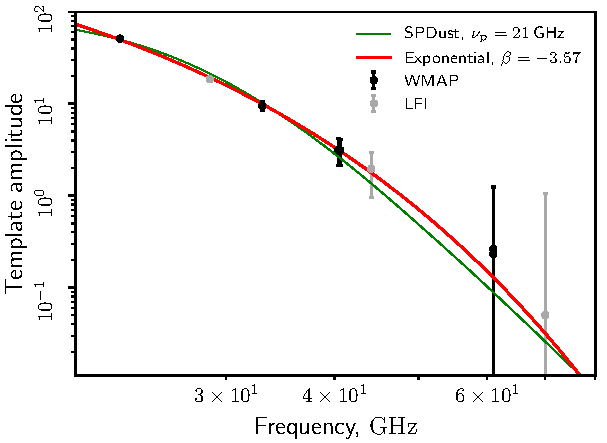
\includegraphics[width=\linewidth]{figures/tempfit_AME_single_v1.pdf}
%	\caption{AME exponential}
%\end{figure}

\subsection{Posterior distribution and Gibbs sampling}

As shown in \citet{bp01}, this parametric description of the instrumental effects and skythis parametric description of the instrumental effects and sky  allows us to write down a total model for the data, $\boldsymbol d=\boldsymbol s^\mathrm{tot}(\boldsymbol\omega)+\boldsymbol n^\mathrm w$, where $\boldsymbol s^\mathrm{tot}$ encompasses all of the terms in Eq.~\eqref{eq:model} except for the white noise term. Assuming that all instrumental effects have been modelled, the data should be Gaussian distributed with a mean of $\boldsymbol s^\mathrm{tot}(\boldsymbol\omega)$ and variance $\boldsymbol \sigma_0^2$. Given this model, we can evaluate the likelihood for arbitrary chunks of time-ordered data in the context of the entire model, so that individual chunks of data with poor fits can be more easily identified. In general, the likelihood is written
\begin{equation}
	P(\boldsymbol d\mid\boldsymbol\omega)\propto\exp\left(-\frac12\sum_t\frac{(d_t-s^\mathrm{tot}_t(\boldsymbol\omega))^2}{\sigma_0^2}
	\right).
\end{equation}
If $\boldsymbol d\sim\mathcal N(\boldsymbol s^\mathrm{tot},\boldsymbol\sigma_0^2)$ is the correct model for the data, the argument of the exponent is proportional to a $\chi^2$-distribution with $n_\mathrm{TOD}$ degrees of freedom. In the limit of large $n$, a $\chi^2$ distribution is well-approximated by a Gaussian with mean $n$ and variance $2n$. Therefore we define and use the reduced-$\chi^2$ statistic,
\begin{equation}
	\chi^2\equiv \frac{\sum_t((d_t-s_t^\mathrm{tot})^2/\sigma_0^2 - n_\mathrm{TOD}}{\sqrt{2n_\mathrm{TOD}}},
\end{equation}
which is approximately drawn from the standard normal distribution $\mathcal N(0,1)$.

The \cosmoglobe\ Gibbs chain is given by
\begin{alignat}{10}
\label{eq:gain_samp_dist}\g &\,\leftarrow          P(\g&\,               \mid \d, &\,    &          &\,\boldsymbol\xi_n,  &\,\boldsymbol s^\mathrm{inst}, &\,\boldsymbol\beta, &\,\boldsymbol a, &\,C_{\ell},&\,\boldsymbol\theta)\\
\label{eq:ncorr_samp_dist} \ncorr &\,\leftarrow    P(\ncorr&\,           \mid \d, &\,\g, &\,        &\,\boldsymbol\xi_n,  &\,\boldsymbol s^\mathrm{inst}, &\,\boldsymbol\beta, &\,\boldsymbol a, &\,C_{\ell},&\,\boldsymbol\theta)\\ 
\label{eq:xi_samp_dist} \boldsymbol\xi_n &\,\leftarrow        P(\boldsymbol\xi_n&\,            \mid \d, &\,\g, &\,\ncorr, &\,        &\,\boldsymbol s^\mathrm{inst}, &\,\boldsymbol\beta, &\,\boldsymbol a, &\,C_{\ell},&\,\boldsymbol\theta)\\
\label{eq:samp_inst}\boldsymbol s^\mathrm{inst} &\,\leftarrow                                 P(\boldsymbol s^\mathrm{inst}&\,             \mid \d, &\,\g, &\,\ncorr, &\,\boldsymbol\xi_n,  &\,      &\,\boldsymbol\beta, &\,\boldsymbol a, &\,C_{\ell},&\,\boldsymbol\theta)\\
\label{eq:beta_samp}\boldsymbol\beta &\,\leftarrow                     P(\boldsymbol\beta&\, \mid \d, &\,\g, &\,\ncorr, &\,\boldsymbol\xi_n,  &\,\boldsymbol s^\mathrm{inst}, &\,       &\,    &\,C_{\ell},&\,\boldsymbol\theta)\\
\boldsymbol a &\,\leftarrow                                   P(\boldsymbol a&\,               \mid \d, &\,\g, &\,\ncorr, &\,\boldsymbol\xi_n,  &\,\boldsymbol s^\mathrm{inst}, &\,\boldsymbol\beta, &\,    &\,C_{\ell},&\,\boldsymbol\theta)\\
C_{\ell} &\,\leftarrow                             P(C_{\ell}&\,         \mid \d, &\,\g, &\,\ncorr, &\,\boldsymbol\xi_n,  &\,\boldsymbol s^\mathrm{inst}, &\,\boldsymbol\beta, &\,\boldsymbol a,&\,\phantom{C_{\ell}}&\,\boldsymbol\theta)&\label{eq:cl_sampling}\\
\boldsymbol\theta &\,\leftarrow                             P(\boldsymbol\theta&\,         \mid \d, &\,\g, &\,\ncorr, &\,\boldsymbol\xi_n,  &\,\boldsymbol s^\mathrm{inst}, &\,\boldsymbol\beta, &\,\boldsymbol a,&\,C_\ell\phantom{,}&\phantom{\,\boldsymbol\theta})\label{eq:param_samp},
\end{alignat}
with each step requiring its own dedicated sampling algorithm, and in the case of \bp, its own publication. The \commanderthree\ pipeline is designed so that results of each Gibbs sample can be easily passed to each other, and that the internal calculations of each step do not directly depend on the inner workings of each other. Therefore, in order to add another data set to the Gibbs chain, one must implement Eqs.~\eqref{eq:gain_samp_dist}--\eqref{eq:samp_inst} for each instrument, as was done in \citet{bp01} and \citet{bp10} for \Planck\ LFI and in \citet{bp17} for \WMAP, or simply pass processed maps with beam, mask, and noise information to Eqs.~\eqref{eq:beta_samp}--\eqref{eq:param_samp}, as was done for the Haslam 408\,MHz map \citep{haslam1982,remazeilles2014} and the \Planck\ 353 and 857\,GHz maps.

Before we discuss the results of this Gibbs chain as applied to the \Planck\ LFI and \WMAP\ data, we summarize the TOD processing steps in Sect.~\ref{sec:algorithms}.



\subsection{Sampling algorithms}
\label{sec:algorithms}

Each step of the Gibbs chain requires its own distribution to be sampled from. In Sect.~\ref{ssec:oldsamplers} we review the sampling algorithms implemented in the \bp\ suite of papers, while Sects.~\ref{ssec:mapmaking}--\ref{ssec:baseline} provide an overview of the \WMAP-specific processing steps.

\subsubsection{Review of sampling algorithms}
\label{ssec:oldsamplers}


Several of the techniques required for \WMAP\ data analysis have already been implemented and describe in the \bp\ framework and implemented in \commanderthree. This section includes a summary of the algorithms that were used described previously for the analysis of LFI data. In each of these cases, every part of the model not explicitly mentioned is held fixed unless specified otherwise.

Noise estimation and calibration, described in \citet{bp06} and \citet{bp07} respectively, are highly degenerate, given that the timestream
\begin{equation}
	d_{t,i}=g_{q,i}s_{t,i}^\mathrm{tot}+n_{t,i}^\mathrm{corr}+n_{t,i}^\mathrm{wn}
\end{equation}
is equally well fit by two solutions if $g'=gs^\mathrm{tot}/(s^\mathrm{tot})'$ or ${(n^\mathrm{corr})'=n^\mathrm{corr}+gs^\mathrm{tot}+g'(s^\mathrm{tot})'}$. In practice, this is dealt with by marginalizing over the correlated noise realization $\boldsymbol n^\mathrm{corr}$ assuming a fixed PSD $\boldsymbol\xi_n$, so that Eqs.~\eqref{eq:gain_samp_dist} and \eqref{eq:ncorr_samp_dist} are evaluated as
\begin{alignat}{10}
	\g&\,\leftarrow P(\g&\,\mid\d, &\, &\,&\,\boldsymbol\xi_n,\ldots)
	\label{eq:gmarg}
	\\
	\ncorr&\,\leftarrow P(\ncorr&\,\mid\d, &\,\g, &\,&\,\boldsymbol\xi_n,\ldots).
	\label{eq:ncorr_only}
\end{alignat}
This is allowed by probability theory given that the joint distribution $P(\g,\ncorr\mid\boldsymbol\omega)=P(\ncorr\mid\g,\boldsymbol\omega)P(\g\mid\boldsymbol\omega)$, so that Eqs.~\eqref{eq:gmarg} and \eqref{eq:ncorr_only} evaluated in sequence is equivalent to drawing a joint sample from $P(\g,\ncorr\mid\boldsymbol\omega)$. In practice, this means that when sampling for $\g$, the covariance matrix $\mathsf N=\mathsf N_\textrm{wn}+\mathsf N_\textrm{corr}$ must be used, rather than just $\mathsf N_\mathrm{wn}$.

\commanderthree\ models the gain at each timesteam $t$ for a detector $i$ as
\begin{equation}
	g_{t,i}=g_0+\Delta g_i+\delta g_{q,i}
\end{equation}
where $q$ labels the time interval for which we assume the gain is constant over, e.g., a single scan. In order to sample the gain, we write down a generative model for the TOD,
\begin{equation}
	\d_i=\g_{i}\s_{i}^\mathrm{tot} +\n_{i}^\mathrm{tot}\sim\mathcal N(\g_i\s_{i}^\mathrm{tot},\mathsf N_i).
\end{equation}
Since the $\d_i$ is given as a linear combination of the fixed signal and the gains, a random sample of the gain can be drawn by solving\footnote{See, e.g., Appendix A.2 of \citet{bp01} for a derivation of this result.}
\begin{equation}
	\label{eq:gain_gauss_samp}
	[(\s_i^\mathrm{tot})^T\mathsf N_i^{-1}\s_i^\mathrm{tot}]\g_i
	=(\s_i^\mathrm{tot})^T\N^{-1}_i\d_i
	+(\s_i^\mathrm{tot})^T\N^{-1/2}_i\boldsymbol\eta.
\end{equation}
Note that the $\mathsf N_i$ depends implicitly on the noise PSD $\boldsymbol \xi_n$, while the specific realization of $\ncorr$ is accounted for in the covariance matrix.
In practice, as shown in \citet{bp07}, \commanderthree\ samples $g_0$, $\Delta g_i$, and $\delta g_{q,i}$ in separate sampling steps. Formally, the Gibbs chain is broken by fitting the absolute gain $g_0$ to the orbital dipole rather than the full sky signal. However, this makes the sampling much more robust to unmodelled systematic effects, so the trade-off in rigor is justified.

The correlated noise sampling, described in \citet{bp06}, follows a similar procedure to gain sampling, except now conditioned upon the gain estimate, sampled just before correlated noise in the code. Similar to the gain case, we can write a generative model for the data
\begin{equation}
	\d_i=\g_i\s_i^\mathrm{tot}+\n_i^\mathrm{corr}+\n^\mathrm{wn}_i
	\sim\mathcal N(\g_i\s_i^\mathrm{tot},\N_{\mathrm{corr},i}+\N_{\mathrm{wn},i}).
\end{equation}
Given fixed $\boldsymbol r_i=\d_i-\g_i\s_i^\mathrm{tot}$, we can again write a sampling equation, 
\begin{equation}
	\label{eq:ncorr_gauss_samp}
	(\N_{\mathrm{corr},i}^{-1}+\N_{\mathrm{wn},i}^{-1})
	\n^\mathrm{corr}_i
	=\N^{-1}_{\mathrm{wn},i}\boldsymbol r_i
	+\N^{-1/2}_{\mathrm{wn},i}\boldsymbol\eta_1
	+\N^{-1/2}_{\mathrm{corr},i}\boldsymbol\eta_2.
\end{equation}
This gives a sample of the true underlying correlated noise that occurred when the instrument was taking data. In practice, this is equivalent to the destriping mapmaking algorithm \texttt{Madam}, and returns equivalent results to the classical method \citep{bp02}.

To solve for the correlated noise parameters, we assume that the correlated noise is drawn from a correlated Gaussian and form the posterior distribution
\begin{equation}
	P(\boldsymbol\xi_n\mid\n^\mathrm{corr})\propto\frac{\exp{[-\frac12(\n^\mathrm{corr})^T\N_\mathrm{corr}^{-1}\n^\mathrm{corr}]}}
	{\sqrt{|\N_\mathrm{corr}|}}P(\boldsymbol\xi_n).
\end{equation}
The simplest parameterization for correlated noise is given by
\begin{equation}
	\mathsf N_\mathrm{corr}(f)=\sigma_0^2\left(\frac f{f_\mathrm{knee}}\right)^\alpha.
\end{equation}
This can in principal be modified, and for \Planck\ LFI a Gaussian log-normal bump was added at a late stage in the \bp\ analysis. Rather than sampling for $\sigma_0$, we effectively fix the white noise level to the noise level at the highest frequency, e.g.,
\begin{equation}
	\sigma_0^2\equiv\frac{\mathrm{Var}(r_{t+1}-r_t)}2,
\end{equation}
where $t$ and $t+1$ are consecutive time samples, and ${\boldsymbol r\equiv\boldsymbol d-\boldsymbol g\boldsymbol s^\mathrm{tot}
-\boldsymbol n^\mathrm{corr}}$. In practice, this makes $\sigma_0$ a deterministic function of the sampled sky and gain parameters. The parameters $\alpha$ and $f_\mathrm{knee}$ are not linear in the data, so must be sampled using the general inversion sampler.\footnote{See, e.g., Appendix A.3 of \citet{bp01} and Chapter 7.3.2 of \citet{numerical_recipes} for further details.} In practice, this requires gridding out the posterior one parameter at a time.

The bandpass mismatch is explicitly modeled in \commanderthree. Using the calibrated sky model, the expected calibrated sky signal is given by
\begin{equation}
	m_{p,j}=\mathsf B_{p,p'}\sum_c\mathsf M_{c,j}a^c_{p'}+n_{j,p}^\mathrm w.
\end{equation}
Since $\mathsf M_{c,j}$ encodes the bandpass response of every detector $j$ to every component $c$, the maps $\boldsymbol m_j$ will each be slightly different depending on their bandpass $\tau_j$. More importantly, differences in signal between different detectors can be attributed to a spurious polarization signal, giving spurious polarized maps. Therefore, before averaging different detectors together, \commanderthree\ estimates the average over all detectors in a given frequency channel $\boldsymbol m\equiv \langle \boldsymbol m_j\rangle$, and subtracts it directly in the timestream;
\begin{equation}
	\delta s_{t,j}^\mathrm{leak}=\mathsf P_{t,p}^j\mathsf B_{p,p'}^j\left(\boldsymbol m_{j,p'}-\boldsymbol m_{p'}\right).
\end{equation}
This leakage term uses the expected bandpass

Once the instrumental parameters have been sampled, \commanderthree\ computes the calibrated TOD for each band,
\begin{equation}
	r_{t,j}=\frac{d_{t,j}-n_{t,j}^\mathrm{corr}}{g_{t,j}}-\left(s_{t,j}^\mathrm{orb}
	+s_{t,j}^\mathrm{fsl}+\delta s_{t,j}^\mathrm{leak}+s_{t,j}^\mathrm{inst}\right)
\end{equation}
where $\s^\mathrm{orb}$ is the orbital dipole, $\s^\mathrm{fsl}$ is the far sidelobe timestream, $\delta\s^\mathrm{leak}$ is the bandpass leakage, and $\s^\mathrm{inst}$ is the set of instrumental parameters, e.g., the 1\,Hz spike in LFI. With the a correlated noise realization removed, one can perform simple binned mapmaking, weighting each pixel by the white noise amplitude.

Component separation for intensity and polarization are described in \citet{bp13} and \citet{bp14}, respectively.

% Power spectrum estimation is described in \citet{bp12}.

% Cosmological parameter estimation is described in \citet{bp11}.


\subsubsection{Differential mapmaking}
\label{ssec:mapmaking}

The first additional algorithm that needed to be added to \commanderthree\ was differential mapmaking, since the \Planck\ LFI data came from a standard single-horn instrument.  

After calibration and correction for instrumental effects, the TOD can be modeled as
\begin{equation}
	\boldsymbol d=\mathsf P\boldsymbol m+\boldsymbol n^\mathrm{w},
\end{equation}
where
\begin{equation}
	\boldsymbol m=\mathsf B^\mathrm{symm}\mathsf M\boldsymbol a
\end{equation}
is the expected map for each detector after removing the orbital dipole, far sidelobe, baseline, and a realization of correlated noise. The differential pointing strategy can be represented in matrix form as 
\begin{align}
	\label{eq:wmap_pointing}
	\mathsf P_{tp}&=
	(1+x_\mathrm{im})(\delta_{p^I_{\phantom\A}p_\A^I}
	+\delta_{p^Q_{\phantom\A}p^Q_\A}\cos2\psi_\A
	+\delta_{p^U_{\phantom\A}p^U_\A}\sin2\psi_\A)
	\\
	&-(1-x_\mathrm{im})(\delta_{p^I_{\phantom\B}p_\B^I}
	-\delta_{p^Q_{\phantom\A}p^Q_\B}\cos2\psi_\B
	-\delta_{p^U_{\phantom\A}p^U_\B}\sin2\psi_\B)
\end{align}
where $p_\A$ and $p_\B$ are the time-dependent pointings for each DA. The maximum likelihood map can in principal be solved using the usual mapmaking equation,
\begin{equation}
	\label{eq:mapmapking_eqn1}
	\mathsf P^T\mathsf N^{-1}\mathsf P\boldsymbol m=\mathsf P^T\mathsf N^{-1}\boldsymbol d.
\end{equation}
For a single-horn experiment, i.e., \Planck\ LFI, this reduces to a $3\times3$ matrix that can be inverted for each pixel independently. For the pointing matrix in Eq.~\eqref{eq:wmap_pointing}, this is no longer possible, as there is inherently coupling between horns A and B in the timestreams. The $3N_\mathrm{pix}\times3N_\mathrm{pix}$ matrix can be solved using an iterative algorithm, e.g., preconditioned conjugate gradients.

\citet{jarosik2010} identified an issue where a large difference in the sky temperature at pixel value at pixel A versus pixel B induced artifacts in the mapmaking procedure. We adopt the procedured first described in \citet{hinshaw2003a} where only the pixel in a bright region, defined by a small processing mask \citep{bennett2012} is accumulated, thus modifying the mapmaking equation to
\begin{equation}
	\mathsf P^T_\mathrm{am}\mathsf N^{-1}\mathsf P\boldsymbol m
	=\mathsf P^T_\mathrm{am}\mathsf N^{-1}\boldsymbol d.
\end{equation}
This equation can be solved using the BiCG-STAB algorithm for a non-symmetric matrix $\mathsf A$ where $\mathsf A\boldsymbol x=\boldsymbol b$. We apply a preconditioner $\mathsf M$ by numerically inverting the same problem with $N_\mathrm{side}=16$ maps and applying a diagonal noise matrix. Numerically, we define convergence as when the residual $\boldsymbol r\equiv\boldsymbol b-\mathsf A\boldsymbol x$ satisfies $\boldsymbol r^T\mathsf M^{-1}\boldsymbol r/\boldsymbol b^T\mathsf M^{-1}\boldsymbol b<10^{-10}$, which typically takes about 20 iterations for producing frequency maps.


\subsubsection{Transmission imbalance estimation}
\label{ssec:imbalance}


Transmission imbalance, i.e., the differential power transmission of the optics and waveguide components, can be parameterized as
\begin{equation}
	d_{t,j}=g_{t,j}[(1+x_{\mathrm{im},j})s_{t,j}^\mathrm{tot,A}-(1-x_{\mathrm{im},j})s_{t,j}^\mathrm{tot,b}]+n_t.
\end{equation}
This can be decomposed into a differential (d) and common-mode (c) signal such that
\begin{equation}
	d_{t,j}=g_{t,j}[s_{t,j}^\mathrm d+x_{\mathrm{im},j}s_{t,j}^\mathrm c]+n_t.
\end{equation}
In this form, the imbalance parameters can be estimated by drawing Gaussian samples from the standard mean and standard deviation over the entire mission. To draw samples for $x_{\mathrm{im},j}$, we construct the sampling routine analogous to Eqs.~\eqref{eq:gain_gauss_samp} and \eqref{eq:ncorr_gauss_samp} with $\boldsymbol r=\boldsymbol d-\boldsymbol g\boldsymbol s^\mathrm d$,
\begin{equation}
	[(\boldsymbol g\boldsymbol s^\mathrm c)^T\mathsf N^{-1}\boldsymbol g\boldsymbol s^\mathrm c]x_\mathrm{im}
	=(\boldsymbol g\boldsymbol s^\mathrm c)^T\mathsf N^{-1}\boldsymbol r+(\boldsymbol g\boldsymbol s^\mathrm c)^T\mathsf N^{-1/2}\boldsymbol\eta,
\end{equation}
essentially cross-correlating the common-mode signal with $\boldsymbol r$ with appropriate weights and adding a Gaussian random variable with the correct weighting. Note that we are marginalizing over the correlated noise here by using $\N=\N_\mathrm{wn}+\N_\mathrm{corr}$. This mitigates any baseline drifts being erroneusly attributed to the common-mode signal and biasing the estimate of $x_\mathrm{im}$.

The \WMAP\ procedure, described in \citet{jarosik2003a}, fit for common-mode and differential coefficients along with a cubic baseline over 10 precession periods at a time, corresponding to 10 hours of observation. The mean and uncertainty were then calculated by averaging and taking the standard deviation of these values. This approach has the benefit of allowing for the tracking of possible transmission imbalance variation throughout the mission. However, none of the \WMAP\ suite of papers have indicated this, and it has not arisen in our analysis, so we model this as an effect whose value is constant throughout the mission.

\subsubsection{Baseline sampling}
\label{ssec:baseline}

The data model adopted in \citet{hinshaw2003a} can be written in raw digital units (du) as
\begin{equation}
	\d = \mathsf{GPBM}\boldsymbol a+\boldsymbol n+\boldsymbol b,
\end{equation}
where $\boldsymbol b$ is the instrumental baseline and $\boldsymbol n$ is the
total instrumental noise. As detailed in \citet{bp06}, \commanderthree\ divides
the noise into $\n=\n^\mathrm w+\n^\mathrm{corr}$, a white noise term and a
correlated noise term. By definition, the white noise does not have any
correlations between adjacent pixels, so that any pixel-pixel covariance should
be fully described by realizations of the $\n^\mathrm{corr}$ timestream.

\commander\ estimates the baseline using the full estimate of the current sky
model, $\boldsymbol r=\boldsymbol d-g\boldsymbol s^\mathrm{tot}=\boldsymbol
b+\boldsymbol n$. Modeling $\boldsymbol b=b_0+b_1\Delta t$, we solve for $b_0$
and $b_1$ using linear regression in each timestream while masking out samples
that lie within the processing mask. Strictly speaking, this is breaking the
Gibbs chain, as we are not formally sampling $b_0$ and $b_1$ for each TOD
chunk. In practice, baseline estimation uncertainty propagates to correlated
noise realizations and PSD parameters, as discussed below.

The approach detailed in \citet{hinshaw2003a} and the \commander\
implementation differ mainly in the assumed stable timescale -- the initial
\WMAP\ baseline is estimated over one hour timescales, whereas \commander\
assumes constant values throught the entire timestream, 3--7 days depending on
the band in question. As noted in \citet{hinshaw2003a}, residual baseline
variations manifest as correlated noise stripes in the final maps. \WMAPnine\
solves this using a time-domain filter, downweighting the data based off of the
noise characterization. This approach is equivalent to the \commanderthree\
procedure of removing a constrained realization of correlated noise from the
timestream directly, based on the best-fit to the noise PSD.

%\subsubsection{Other things we have added?}
%\label{ssec:baseline}



%\subsection{\planck\ LFI data processing}
%\label{ssec:lfi}

%Summary of \citet{bp01}, \citet{bp10}.
%Artem was here...

%\subsection{\wmap\ data processing}
%\label{ssec:wmap}

%As summarized in \citet{bp17}, the TOD processing for \WMAP\ has been
%implemented in the \commanderthree\ Gibbs sampling framework.  The process of
%implementing this module in \commanderthree\ generally involved implementing
%the procedures outlined in \citet{jarosik2003a}, \citet{hinshaw2003a},
%\citet{jarosik2007}, and \citet{wmapexsupp}, and implementing a sampling
%algorithm whenever an estimate based off of the data was obtained. \citet{bp17}
%found excellent agreement between our processed maps and the official
%\WMAPnine\ products. The most visually obvious exception is that the
%\citet{bp17} maps have no trace of the poorly-measured modes induced by
%transmission imbalance uncertainties. Although \citet{bp17} focused on the
%\Q-band maps, we show in Sect.~\ref{sec:freqmaps} that this is representative
%of all \WMAP\ bands, with the notable exception of \K-band.

%The data model adopted in \citet{hinshaw2003a} can be written in raw digital units (du) as
%\begin{equation}
%	\d = \mathsf{GPBM}\boldsymbol a+\boldsymbol n+\boldsymbol b,
%\end{equation}
%where $\boldsymbol b$ is the instrumental baseline and $\boldsymbol n$ is the
%total instrumental noise. As detailed in \citet{bp06}, \commanderthree\ divides
%the noise into $\n=\n^\mathrm w+\n^\mathrm{corr}$, a white noise term and a
%correlated noise term. By definition, the white noise does not have any
%correlations between adjacent pixels, so that any pixel-pixel covariance should
%be fully described by realizations of the $\n^\mathrm{corr}$ timestream.

%Three notable deviations from the official \WMAPnine\ pipeline and the
%\cosmoglobe\ approach are the gain estimation, the correlated noise treatment,
%and the data fraction used.  The \WMAPnine\ gain solution was a parametric fit
%to the orbital dipole measurements as a function of the instrumental
%housekeeping parameters, as detailed in Appendix~A of \citet{wmapexsupp}. This
%approach avoids the dependence of a robust Galactic foreground model, and
%requires both excellent knowledge of the radiometers and a clean orbital dipole
%measurement which can be compared to the known signal. \commanderthree's
%sampling approach, as summarized in \citet{bp07}, fits the average gain over
%all detectors and TOD samples to the orbital dipole. In addition,
%\commanderthree\ calibrates deviations from the average gain as a function of
%detector and time to the total sky model.  This approach is highly dependent on
%using a sky model that accurately reflects the data, but makes fewer
%assumptions regarding the behavior of the detectors in relation to the
%housekeeping parameters. 













%\subsection{Calibration}

%In order to get the raw data into the sky units $\mathrm{mK_{CMB}}$, it is necessary to make a quantitative assessment of the data's goodness-of-fit. To do this, we use mapped time-domain residuals of the timestream based on an initial sky model. Following the procedure of \citet{bp06}, we create a smoothed map of the absolute deviation of the model from the sky signal. The residual maps were first smoothed to $3^\circ$, the absolute value was taken, and then the map was smoothed again with a $15^\circ$ beam. This procedure gave us an indication of the regions of the sky that are not fully characterized by the sky model. We then evaluated the \texttt{Cosmoglobe} Sky model\footnote{\url{cosmoglobe.readthedocs.io}} associated with the \BP\ data release\footnote{\url{beyondplanck.science}} to create a map of the expected thermal dust, AME, free-free, and radio emission at each \WMAP\ frequency. We thresholded using the 80th percentile of this map to match the residual map. The combination of this sky model-informed mask and the residual-informed mask formed the main processing mask for the calibration and correlated noise analysis.
%Outside of these mask, the data are fit will by the sky model, so the calibration and the correlated noise estimates should both be unbiased.



\section{Data and data processing}
\label{sec:data}

We describe the delivered \WMAP\ data in Sect.~\ref{sec:products}, then describe the treatment we apply it to make them compatible with \commanderthree\ in Sect.~\ref{sec:preprocessing}, then describe the computational requirements in Sect.~\ref{sec:resources}.

\subsection{Publicly available \WMAP\ products}
\label{sec:products}

The full \WMAP\ dataset is hosted at the Legacy Archive for Microwave Backgroudn Data Analysis (LAMBDA).\footnote{\url{https://lambda.gsfc.nasa.gov/product/wmap/dr5/m_products.html}} In addition to the primary scientific products, e.g., cosmological parameters, CMB power spectra and anisotropy maps, and frequency maps, the time-ordered data (TOD) can be downloaded, both in uncalibrated and calibrated form.\footnote{\url{https://lambda.gsfc.nasa.gov/product/wmap/dr5/tod_info.html}} In principle, thanks to these data and the explanatory supplements \citep{wmapexsupp}, the entire data analysis pipeline can be reproduced from TOD in digital units (du) to frequency maps.

For this analysis, we keep certain instrumental parameters fixed to the reported values. For example, we have made no attempts to rederive the pointing solutions, re-estimate the main beam response and far sidelobe pickup, or recover data that was flagged in the \WMAP\ event log. These and other analyses, such as estimating the bandpass shift over the course of the mission, are certainly possible within the larger Gibbs sampling framework. However, in this work we limit ourselves to recalibrating the TOD, estimating the noise properties, and applying bandpass corrections to the data before mapmaking.

\subsection{TOD pre-processing and data selection}
\label{sec:preprocessing}

\begin{table}
\caption{Flagging statistics}              % title of Table
\label{table:flagged_data}      % is used to refer this table in the text
\centering                                      % used for centering table
\begin{tabular}{c r r r}          % centered columns (4 columns)
\hline\hline                        % inserts double horizontal lines
	Band & Flagged (\%) & Discarded (\%) & Used (\%) \\    % table heading
\hline                                   % inserts single horizontal line
	\K  &  1.72 & 0.87 & 97.4\\
	\Ka &  1.64 & 0.88 & 97.5\\      % inserting body of the table
	\Q1 &  1.84 & 0.84 & 96.5\\
	\Q2 &  1.62 & 0.81 & 97.6\\
	\V1 &  1.62 & 1.10 & 97.3\\
	\V2 &  1.61 & 1.01 & 97.4\\
	\W1 &  1.76 & 1.03 & 97.2\\
	\W2 &  1.60 & 0.81 & 97.6\\
	\W3 &  1.61 & 0.87 & 97.5\\
	\W4 &  1.60 & 0.81 & 97.6\\
\hline                                             %inserts single line
\end{tabular}
\end{table}


%Compare with Table 2 of \citet{bennett2003a}, Table 1 of \citet{hinshaw2007}, Table 2 of \citet{hinshaw2009}. Total observing efficiency was 98.4\% \citep{bennett2012}

The full nine-year \WMAP\ archive spans from August 10, 2001 to August 10, 2010, with the raw uncalibrated data spanning 626\,GB. A little over 1\,\% of the data were lost or rejected due to incomplete satellite telemetry, thermal disturbances, spacecraft anomalies, and station-keeping maneuvers, with an extra 0.1\,\% rejected due to planet flagging \citep{bennett2003a,hinshaw2007,hinshaw2009,bennett2012}. 
The final results reported in \citet{bennett2012} included roughly 98.4\,\% of the total data volume.
A full accounting of all data cuts can be found in Table~1.8 of \citet{wmapexsupp}. In total, we flag the same data indicated in the fiducial \WMAP\ analysis, and use the same planet flags.

As shown in \citet{bp03}, a large fraction of \commanderthree's computational time is spent performing FFTs on individual scans. Rather than truncating datastreams to have lengths equal to ``magic numbers'' for which \texttt{FFTW} \citep{FFTW05} is fastest, as in \citet{bp03}, 
we split the data into scans of length $2^N$, where $N=22$ for \K--\Q, $N=23$ for \V--\W. This yields scans with lengths of 6.21 days for \K- and \Ka-band, 4.97 days for \Q-band, 7.46 days for \V-band, and 4.97 days for \W-band.
These datastream lengths are short enough to be processed quickly and distributed efficiently across multiple processors, while being long enough to properly characterize the noise properties of the timestreams, whose $f_\mathrm{knee}$'s are on the order $1\,\mathrm{mHz}$. Most importantly, \texttt{FFTW} performs fastest when the datastream is of length $2^N$.

When rechunking the data, timestreams of length $2^N$ were interrupted by events logged in Table~1.8 of \citet{wmapexsupp}.
When we encountered these events, TOD segments that were interrupted by the event were appended to the previous TOD, in most cases creating TODs with lengths $>2^N$. We found that events of length $<2^N$ were too short to accurately estimate the noise PSD parameters. This criterion led us to discard these otherwise useful data. In addition, when $>10\%$ of the TOD was flagged, the large number of gaps in the data made the constrained realizations unreliable, as well as biasing the noise PSD parameters. Together, these two effects led to $\simeq1\%$ of the data to be discarded despite being of acceptable quality. We present the full flagging statistics for our maps in Table~\ref{table:flagged_data}. In total, the \Cosmoglobe\ maps use slightly less data than the \textit{WMAP9} official products, which had a total efficiency of $\simeq98.4\%$ \citep{bennett2012}. The total difference in data volume can be entirely accounted for by the cuts described in this paragraph.




\subsection{Computational resources}
\label{sec:resources}

A key motivation of the \cosmoglobe\ project is to evaluate whether it is feasible to perform a joint analysis of two datasets simultaneously, each with its own particular processing requirements and algorithmic treatment. One of the results from \citet{bp17} was that most of the data processing procedures for  \WMAP\ and \Planck\ LFI overlapped, with the notable exception of mapmaking. While the algorithmic requirements have been discussed in Sect.~\ref{sec:methods}, we have not yet quantified the requirements in terms of RAM and CPU hours. In Table~\ref{tab:resources}, we enumerate the RAM requirements and CPU time for each sampling step using the local cluster at the Institute of Theoretical Astrophysics at the University of Oslo. The node that these numbers come from used 128 cores of an AMD EPYC 7H12, 2.6\,GHz machine with 2\,TB of memory. As \commanderthree\ is parallelized and used 128 cores, wall hours in Table~\ref{tab:resources} can be obtained by dividing by 128.

Despite the relatively small data volume spanned by \WMAP, the CPU time is comparable to each of the LFI channels.  By far the largest reason for this is the mapmaking step, which requires looping over the entire dataset for each matrix multiplication, a process which must be repeated $\sim20$ times. This is vastly sped up by the use of a low resolution preconditioner, reducing the number of iterations by an order of magnitude.

%\textit{(One thing I would like to explain -- why does it take so much longer for TOD operations? My initial thought was that each timestream requires two timestreams for each horn, but that's not enough.)}

Additionally, operations that require creating timestreams for each detector, i.e., TOD projection, sidelobe evaluation, and orbital dipole projection, take much longer than expected from a pure data volume scaling. Part of this is due to each \WMAP\ radiometer needing to evaluate the sky in two pixels simultaneously, doubling the expected workload. The operations of gain sampling and correlated noise sampling include multiple FFTs. Typical LFI TODs are of length $\sim200\,000$, an order of magnitude smaller than the \WMAP\ TODs of length $2^{\text{22\ --\ 23}}$. 

%\textit{(Need to expand ``other'')}

\begin{table*}[t]
  \begingroup
  \newdimen\tblskip \tblskip=5pt
  \caption{Computational resources required for end-to-end
    \cosmoglobe\ processing. All times correspond to CPU hours, and all data volumes are reported in GB. Reported times are
    averaged over more than 100 samples, and vary by $\lesssim\,5\,\%$ from sample to
    sample. %\textbf{Preliminary numbers, not all accurate}
	}
  \label{tab:resources}
  \nointerlineskip
  \vskip -3mm
  \footnotesize
  \setbox\tablebox=\vbox{
    \newdimen\digitwidth
    \setbox0=\hbox{\rm 0}
    \digitwidth=\wd0
    \catcode`*=\active
    \def*{\kern\digitwidth}
    %
    \newdimen\signwidth
    \setbox0=\hbox{-}
    \signwidth=\wd0
    \catcode`!=\active
    \def!{\kern\signwidth}
    %
 \halign{
      \hbox to 5.0cm{#\leaderfil}\tabskip 1em&
      \hfil#\tabskip 1em&
      \hfil#\tabskip 1em&
      \hfil#\tabskip 1em&
      \hfil#\tabskip 1em&
      \hfil#\tabskip 1em&
      \hfil#\tabskip 1em&
      \hfil#\tabskip 1em&
      \hfil#\tabskip 1em&
      \hfil#\tabskip 1em&
      \hfil#\tabskip 1em&
      \hfil#\tabskip 1em&
      \hfil#\tabskip 1em&
      \hfil#\tabskip 1em&
      %\hfil#\tabskip 2em&
      #\tabskip 0em\hfil\cr
    \noalign{\doubleline}
      \omit\textsc{Item}\hfil&
      \omit\hfil\textsc{30}\hfil&
      \omit\hfil\textsc{44}\hfil&
      \omit\hfil\textsc{70}\hfil&
      \omit\hfil\K\hfil&
      \omit\hfil\Ka\hfil&
      \omit\hfil\Q1\hfil&
      \omit\hfil\Q2\hfil&
      \omit\hfil\V1\hfil&
      \omit\hfil\V2\hfil&
      \omit\hfil\W1\hfil&
      \omit\hfil\W2\hfil&
      \omit\hfil\W3\hfil&
      \omit\hfil\W4\hfil&
      \omit\hfil\textsc{Sum}\hfil\cr
      %\omit\hfil\textsc{Sum}\hfil&
      %\omit\hfil\textsc{Reference}\hfil\cr
      \noalign{\vskip 4pt\hrule\vskip 4pt}
      %\noalign{\vskip 8pt}
      \noalign{\vskip 5pt\hrule\vskip 5pt}
        \multispan5\textit{Data volume}\hfil\cr
        \noalign{\vskip 2pt}
        %\hskip 10pt Uncompressed TOD volume                 & {\gray 761 GB} &
        %{\gray 1\,633 GB} & {\gray 5\,522 GB} & {\gray 7\,915 GB}& \cr
	\hskip 10pt Compressed TOD volume & **86& *178& **597& **13& **12& **15& **15& **19& **18& **26&**26& **26& **26& 1\,053\cr
        %\hskip 10pt {\bf Total RAM requirements} &  &  &  & **{\bf1\,520}& \cr      
        \noalign{\vskip 2pt}      
      \multispan5\textit{Processing time (cost per run)}\hfil\cr
      \hskip 10pt TOD initialization/IO time                    &1.8& 2.5& 9.3& 0.3& 0.3& 0.4& 0.4& 0.4& 0.4& 0.5& 0.5& 0.5& 0.5& *17.8\cr
      \hskip 10pt Other initialization                                &  &  &  &  & & & & & & & & & & *13.4\cr
      \hskip 10pt {\bf Total initialization}                          &  &  &  &  & & & & & & & & & & {\bf *31.2}\cr
      \noalign{\vskip 2pt}      
      \multispan5\textit{Gibbs sampling steps (cost per sample)}\hfil\cr
      %\noalign{\vskip 2pt}
      \hskip 10pt Huffman decompression                            & 1.1& 2.1& 10.5& 0.9& 0.8& 1.0& 1.0& 1.3& 1.3& 1.8& 1.8& 1.8& 1.8& *27.2\cr
      \hskip 10pt TOD projection ($\P$ operation)                  & 0.4& 0.9&  4.2& 2.6& 2.6& 3.3& 3.4& 4.3& 4.3& 6.4& 6.3& 6.3& 6.4& *54.0\cr
      \hskip 10pt Sidelobe evaluation                              & 1.0& 2.1&  7.6& 2.9& 2.9& 3.5& 3.5& 4.7& 4.8& 7.0& 6.9& 6.9& 6.9& *60.7\cr
      \hskip 10pt Orbital dipole                                   & 0.9& 1.9& 7.1& 1.3& 1.3& 1.7& 1.7& 2.2& 2.3& 3.4& 3.3& 3.3& 3.3& *33.7\cr
      \hskip 10pt Gain sampling                                    & 0.5& 0.8& 1.9& 0.8& 0.8& 0.5& 0.5& 0.9& 0.9& 0.7& 0.7& 0.7& 0.7& *10.4\cr
      \hskip 10pt 1\,Hz spike sampling                             & 0.3& 0.4& 1.6& & & & & & & & & & & **2.4\cr      
      \hskip 10pt Correlated noise sampling                        & 2.0& 4.0& 21.7& 2.8& 2.9& 3.3& 3.6& 5.1& 5.4& 8.0& 7.7& 7.2& 8.5& *81.3\cr
      \hskip 10pt Correlated noise PSD sampling                    & 4.8& 5.9& 1.5& 0.2& 0.2& 0.3& 0.3 & 0.5& 0.4& 0.7& 0.6& 0.6& 0.7& *16.7\cr
      \hskip 10pt TOD binning ($\P^t$ operation)                   & 0.1& 0.1& 4.0& 0.5& 0.5& 0.7& 0.8& 0.8& 0.8& 1.2& 12& 1.2& 1.2& *13.1\cr
      \hskip 10pt Mapmaking                                        & & & & 6.4& 7.0& 8.9& 8.1& 11.1& 9.5& 14.4& 14.3& 15.3& 16.4& 119.5\cr
      \hskip 10pt Sum of other TOD processing                      & 4.4& 8.6& 44.4& 14.7& 4.6& 5.1& 5.0& 9.4& 7.7& 8.1& 6.8& 8.6& 8.7& 136.1\cr
      \hskip 10pt {\bf TOD processing cost per sample}             & {\bf 15.5}& {\bf 26.8}& {\bf 104.5}&  {\bf 23.0}& {\bf 24.1}& {\bf 27.6}& {\bf 27.9}& {\bf 40.3}& {\bf 37.4}& {\bf 51.7}& {\bf 50.6}& {\bf 51.9}& {\bf 54.6}& {\bf 535.9}\cr
      \noalign{\vskip 2pt}
      \hskip 10pt Amplitude sampling  &&&&&&&&&&&   &  &  & *14.0\cr
      \hskip 10pt Spectral index sampling  &&&&&&&&&&&   &  &  & *25.5\cr
      \noalign{\vskip 2pt}
      \hskip 10pt {\bf Total cost per sample}                  &&&&&&&&&& &   &  &  &  {\bf 581.2}\cr
      \noalign{\vskip 4pt\hrule\vskip 5pt} } }
  \endPlancktablewide \endgroup
\end{table*}





\begin{figure*}
	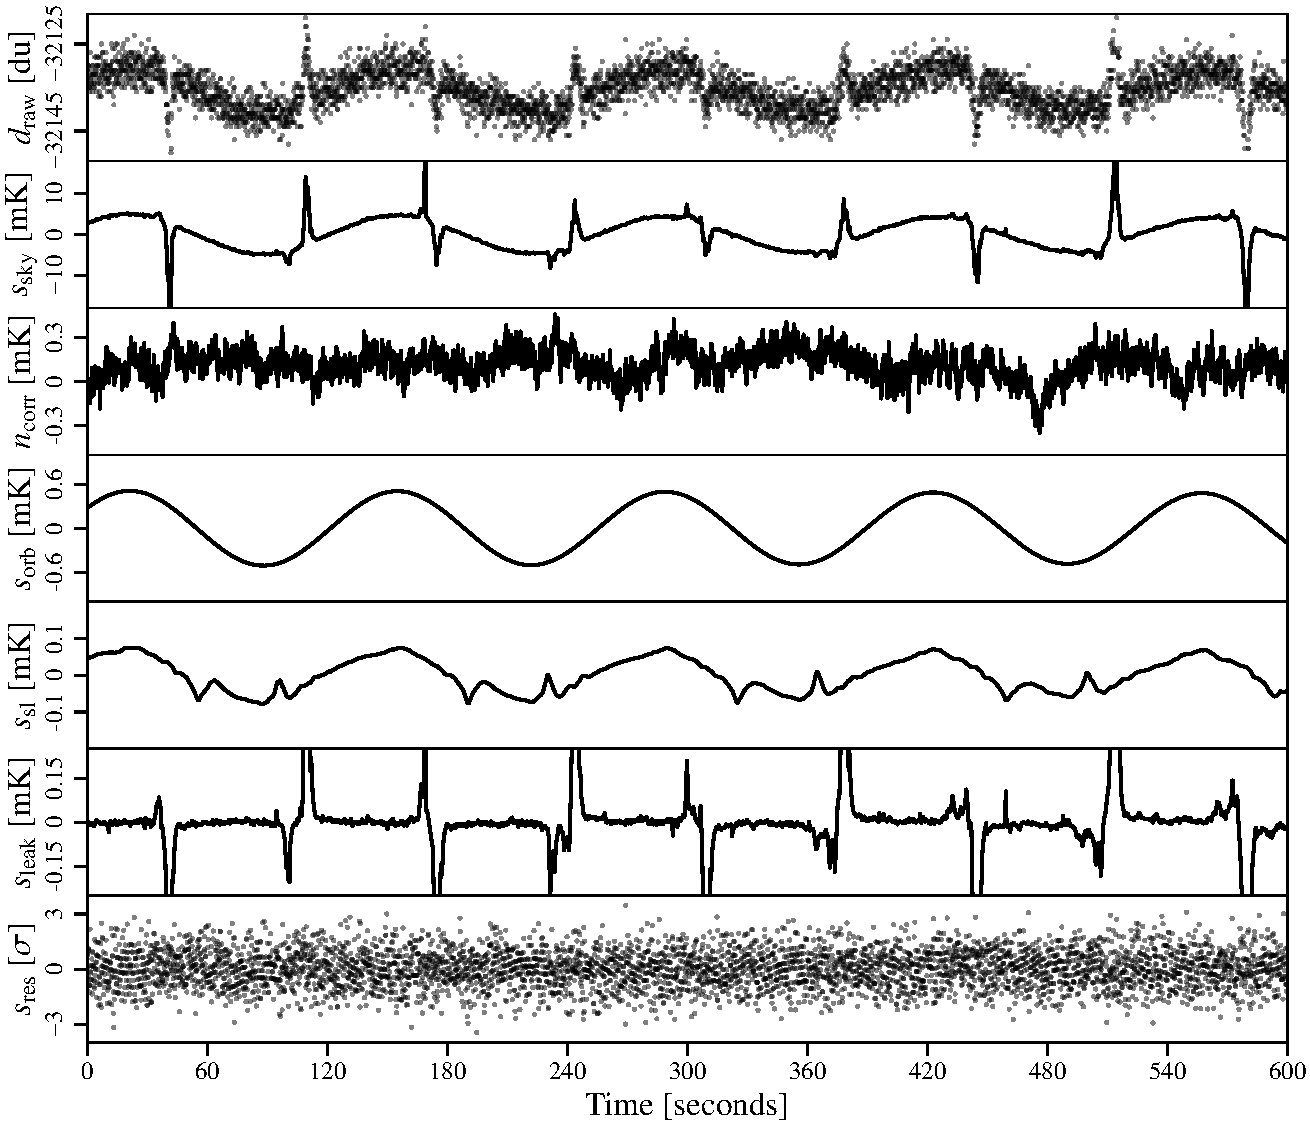
\includegraphics[width=\textwidth]{figures/K113_timestreams.pdf}
	\caption{Each of the timestreams that go into the model. Note the varying dynamic ranges of each plot.}
	\label{fig:timestreams}
\end{figure*}











%\subsection{Calibration}

%In order to get the raw data into the sky units $\mathrm{mK_{CMB}}$, it is necessary to make a quantitative assessment of the data's goodness-of-fit. To do this, we use mapped time-domain residuals of the timestream based on an initial sky model. Following the procedure of \citet{bp06}, we create a smoothed map of the absolute deviation of the model from the sky signal. The residual maps were first smoothed to $3^\circ$, the absolute value was taken, and then the map was smoothed again with a $15^\circ$ beam. This procedure gave us an indication of the regions of the sky that are not fully characterized by the sky model. We then evaluated the \texttt{Cosmoglobe} Sky model\footnote{\url{cosmoglobe.readthedocs.io}} associated with the \BP\ data release\footnote{\url{beyondplanck.science}} to create a map of the expected thermal dust, AME, free-free, and radio emission at each \WMAP\ frequency. We thresholded using the 80th percentile of this map to match the residual map. The combination of this sky model-informed mask and the residual-informed mask formed the main processing mask for the calibration and correlated noise analysis.
%Outside of these mask, the data are fit will by the sky model, so the calibration and the correlated noise estimates should both be unbiased.


%\clearpage





%\subsection{Computational resources}
%\label{sec:resources}


%\section{Low-level posterior distributions}
%\label{sec:lowlevel}

%\clearpage


\section{Posterior distributions}
\label{sec:posteriors}

\begin{figure}[t]
  	\centering
	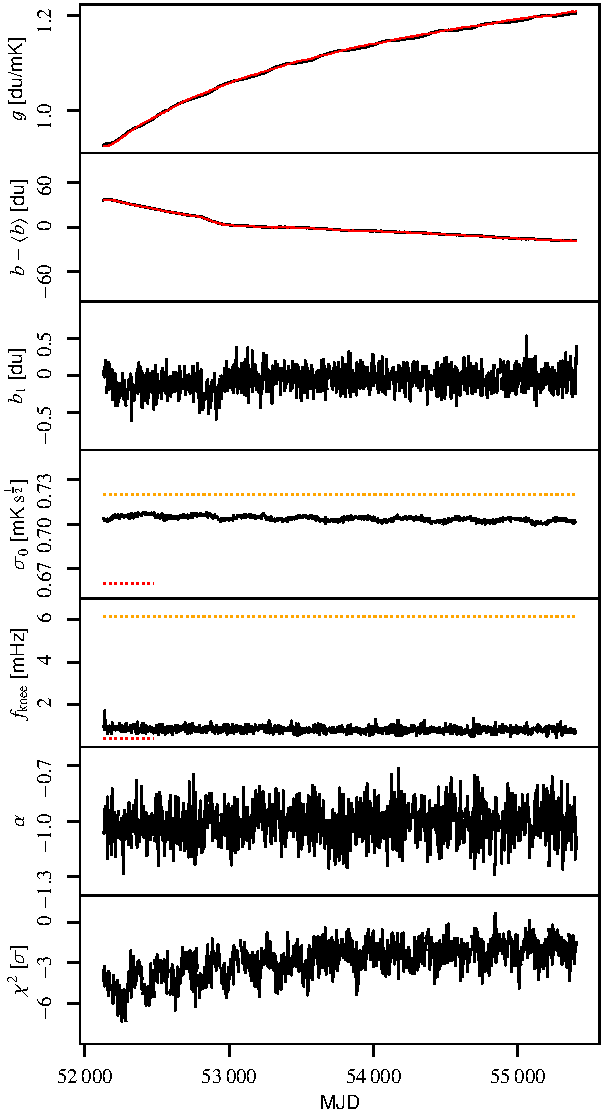
\includegraphics[width=\linewidth]{figures/instpar_CG_K113_v1.pdf}
	\caption{Overview of \K113}
	\label{fig:inst_K113}
\end{figure}

\begin{figure}[t]
  	\centering
	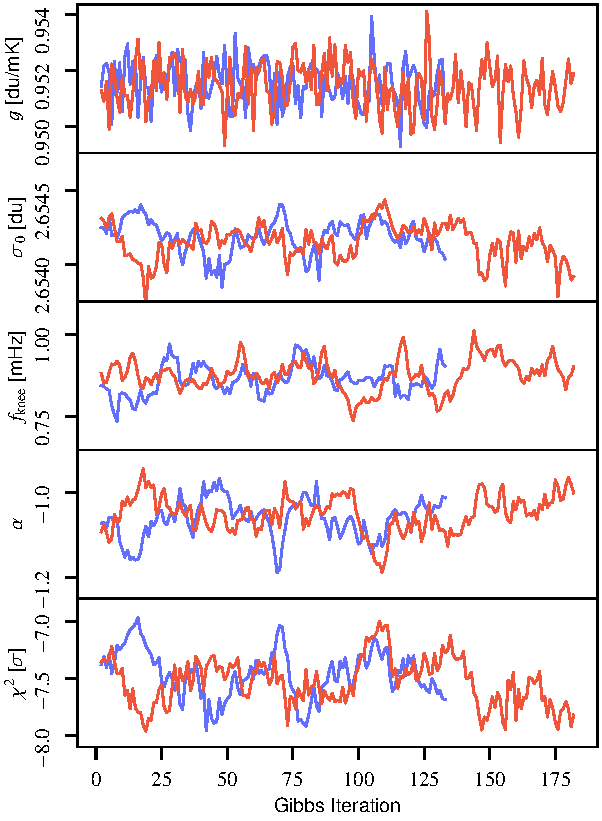
\includegraphics[width=\linewidth]{figures/instpar_CG_K113_samples_v1.pdf}
	\caption{Overview of \K113}
	\label{fig:inst_K113}
\end{figure}



\subsection{Gain and baselines}
\label{sec:gain}

\begin{figure}
	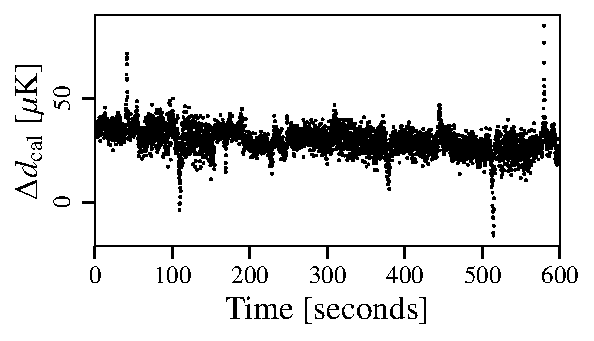
\includegraphics[width=\columnwidth]{figures/K113_TOD_diff_10min.pdf}
	\caption{Difference between the \cosmoglobe\ $\boldsymbol d_\mathrm{cal}=\boldsymbol d/g-\boldsymbol b - \boldsymbol s_\mathrm{sl}$ and the delivered calibrated TOD from \WMAP.}
	\label{fig:cal_comp_10min}
\end{figure}

\begin{figure}
	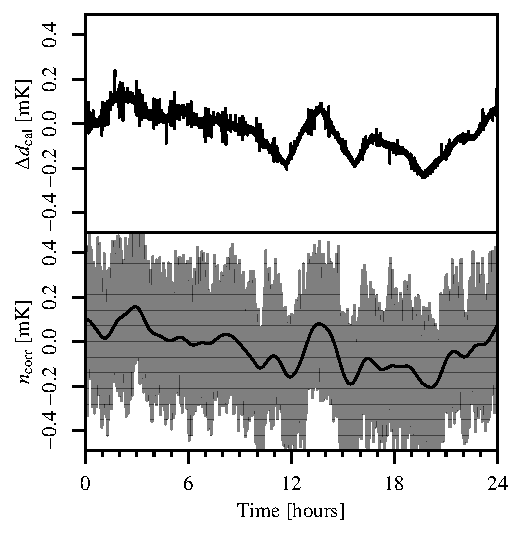
\includegraphics[width=\columnwidth]{figures/K113_TOD_diff_10hr.pdf}
	\caption{(top) Difference between the \cosmoglobe\ $\boldsymbol d_\mathrm{cal}=\boldsymbol d/g-\boldsymbol b - \boldsymbol s_\mathrm{sl}$ and the delivered calibrated TOD from \WMAP. (bottom) Raw correlated noise (gray) and smoothed data with Gaussian kernel (black). This shows more clearly the hourly baseline subtraction from the \WMAP\ treatment.}
	\label{fig:cal_comp}
\end{figure}

To compare the calibrated TODs from \WMAP\ versus \cosmoglobe, it is  important to look at the \WMAP\ gain model,
\begin{equation}
	\label{eq:wmap_gain}
	g=\alpha\frac{\overline V-V_\circ-\beta(T_\mathrm{RXB}-290\,K)}
	{T_\mathrm{FPA}-T_\circ}+(m\Delta t+c),
\end{equation}
where $\alpha$, $\V_\circ$, $\beta$, $T_\circ$, $m$, and $c$ are fit to a constant value across the mission for each radiometer. $\overline V$ are radio frequency bias powers per detector, and $T_\mathrm{RXB}$ and $T_\mathrm{FPA}$ are the receiver box and focal plane assembly temperatures, which are recorded every 23.04\,s. 
Evaluating the model as a function of $T_\mathrm{RXB}$ and $T_\mathrm{FPA}$ requires finding the housekeeping data for the thermistor that was physically closest to the relevant radiometer's focal plane on the satellite. As this requires detailed technical information about the specifications of the telescope layout that can easily be misunderstood, we do not attempt to reproduce the gain model given in Eq.~\eqref{eq:wmap_gain} in this work.
Although we are unable to reproduce the exact gain model parametrized in \citet{wmapexsupp}, the $23.4\,\mathrm s$ time dependence of the gain model on housekeeping data is a plausible explanation for the time-dependent noise variation in the different calibrated data solutions.

As reported in \citet{hinshaw2007}, the calibrated data archive has been calibrated using the procedure listed above, with a baseline subtracted each hour and the sidelobe subtracted. Figure~\ref{fig:cal_comp_10min} shows the \cosmoglobe\ timestream $\boldsymbol d/g-\boldsymbol s_\mathrm{sl}-\boldsymbol b$ with the \WMAP\ delivered calibrated signal subtracted. The most prominent feature is a $\sim25\,\mathrm{\mu K}$ offset, which is unsurprising, given the different treatment of baselines in our two pipelines. The second obvious difference is a series of spikes associated with Galactic plane crossings. The differences of order $50\,\mathrm{\mu K}$ correspond to sky brightness of order $10\,\mathrm{mK}$, equivalent to $\sim0.5\,\%$ deviations in the gain solution. This is twice as large as the 0.2\,\% uncertainty estimated in \citet{bennett2012} based on end-to-end simulations.

On longer timescales, as displayed in Figure~\ref{fig:cal_comp}, the most prominent feature is a signal of amplitude $0.2\,\mathrm{mK}$. This likely due to the hourly baseline subtraction mentioned above, which contrasts with the \cosmoglobe\ approach of assigning a linear baseline solution for the entire scan. However, the variations are commensurate with correlated noise, which for \K113 has $f_\mathrm{knee}\sim0.5\,\mathrm{mHz}$, corresponding to a little over half an hour. Therefore, the hourlong baseline subtraction essentially acts as a destriper, removing an estimate of the correlated noise. To test this hypothesis, we plot a realization of correlated noise generated by \commander, and find that the signals are very similar, both in amplitude and morphology.


We also compare the gain and baseline solutions throughout the course of the mission in Fig.~\ref{fig:inst_K113}. To recover the \WMAPnine\ gain solution, we directly compare the uncalibrated \WMAP\ data with the calibrated \WMAP\ data with a far sidelobe contribution convolved with the delivered \WMAPnine\ DA maps. We find that the calibrated and uncalibrated data can be related by
\begin{equation}
	d^\mathrm{raw}_t=g(d^\mathrm{cal}_t+s^\mathrm{sl}_t)+\sum_{i=0}^3c_i(t-t_0)^i.
\end{equation}
We find that $d^\mathrm{raw}$ is consistent with the expression on the right at the level of $<0.1\,\mathrm{du}$ for all radiometers, suggesting that this estimate of $g$ and the baseline $c_0$ is a good approximation of the \WMAPnine\ calibration solution. An initial estimate using a linear baseline gave an unacceptably poor fit. Given that Eqn.~(2) of \citet{jarosik2003a} employed a cubic baseline fit while fitting for transmission imbalance parameters, it is reasonable to assume that the official calibrated archive was created using a similar procedure.

The morphological characteristics of the \WMAPnine\ and \cosmoglobe\ gain solutions are similar, with a general trend to increase with time. Both solutions also follow a sinusoidal pattern, corresponding to temperature change due to L2's motion around the Sun \citep{wmapexsupp}. However, we do find the amplitude of the \cosmoglobe\ \K-band gain is slightly lower than the \WMAPnine\ solution, and with fewer oscillatory features. Other than the absolute calibration shift in \K-band, the gains are consistent between \cosmoglobe\ and \WMAPnine\ within 1\,\%. For completeness, the full gain comparisons can be found in Fig.~\ref{fig:gain}. 



\subsection{Transmission imbalance}
\label{sec:xim}

The transmission imbalance parameters $x_\mathrm{im}$ are crucial to measure correctly because their mis-estimation can induce a large polarized signal that is coupled to the Solar dipole \citep{jarosik2007,bp17}. The uncertainty in $x_\mathrm{im}$ was quoted as the source of large-scale polarized features in the \WMAPnine\ maps, and a template of this effect was explicitly projected out in the pixel-space polarized covariance matrix. 

We find $x_\mathrm{im}$ values that are largely consistent with the values reported in \citet{bennett2012}, albeit with some outliers. We find in general that the 68\,\% confidence intervals from \cosmoglobe\ are smaller than the fiducial values, although we caution against a direct comparison of these values since such different procedures were used for estimating the uncertainties.

\begin{figure}[t]
  	\centering
	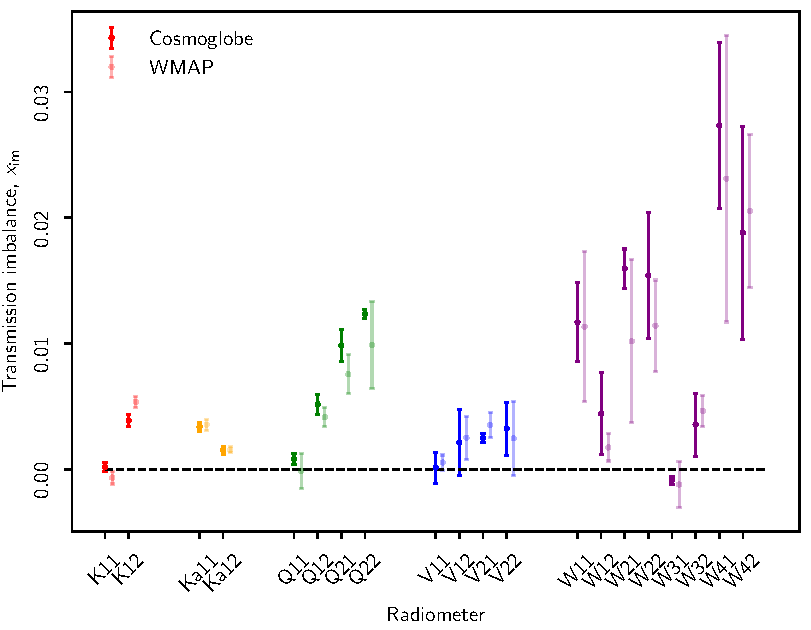
\includegraphics[width=\linewidth]{figures/x_im_CG_v1.pdf}
	\caption{Transmission imbalance}
	\label{fig:x_im}
\end{figure}

%\begin{table}
%\newdimen\tblskip \tblskip=5pt
%\caption{Transmission imbalance parameters for each \WMAP\ radiometer as estimated in the current analysis (\emph{second column}) and in the official 9-year \WMAP\ analysis (\emph{third column}). Our uncertainties indicate $1\,\sigma$ marginal posterior standard deviations. }
%\label{tab:dipole}
%\vskip -8mm
%\footnotesize
%\setbox\tablebox=\vbox{
% \newdimen\digitwidth
% \setbox0=\hbox{\rm 0}
% \digitwidth=\wd0
% \catcode`*=\active
% \def*{\kern\digitwidth}
%%
%  \newdimen\dpwidth
%  \setbox0=\hbox{.}
%  \dpwidth=\wd0
%  \catcode`!=\active
%  \def!{\kern\dpwidth}
%%
%  \halign{\hbox to 1.8cm{#\leaderfil}\tabskip 2em&
%    \hfil$#$\hfil \tabskip 2em&
%    \hfil$#$\hfil \tabskip 0em\cr
%\noalign{\doubleline}
%\omit\hfil\sc Radiometer \hfil& x_{\mathrm{im}}^{\mathrm{CG}}& x_{\mathrm{im}}^{\mathrm{WMAP}}\cr
%\noalign{\vskip 3pt\hrule\vskip 5pt}
%K11 &   0.00018 \pm  0.00013  &  -0.00067 \pm  0.00017 \cr
%K12 &   0.00388 \pm  0.00015  &   0.00536 \pm  0.00014 \cr
%Ka11 &   0.00339 \pm  0.00012  &   0.00353 \pm  0.00017 \cr
%Ka12 &   0.00150 \pm  0.00010  &   0.00154 \pm  0.00008 \cr
%Q11 &   0.00081 \pm  0.00016  &  -0.00013 \pm  0.00046 \cr
%Q12 &   0.00517 \pm  0.00027  &   0.00414 \pm  0.00025 \cr
%Q21 &   0.00985 \pm  0.00042  &   0.00756 \pm  0.00052 \cr
%Q22 &   0.01235 \pm  0.00011  &   0.00986 \pm  0.00115 \cr
%V11 &   0.00012 \pm  0.00041  &   0.00053 \pm  0.00020 \cr
%V12 &   0.00212 \pm  0.00089  &   0.00250 \pm  0.00057 \cr
%V21 &   0.00246 \pm  0.00012  &   0.00352 \pm  0.00033 \cr
%V22 &   0.00323 \pm  0.00070  &   0.00245 \pm  0.00098 \cr
%W11 &   0.01169 \pm  0.00105  &   0.01134 \pm  0.00199 \cr
%W12 &   0.00442 \pm  0.00109  &   0.00173 \pm  0.00036 \cr
%W21 &   0.01595 \pm  0.00052  &   0.01017 \pm  0.00216 \cr
%W22 &   0.01540 \pm  0.00167  &   0.01142 \pm  0.00121 \cr
%W31 &  -0.00089 \pm  0.00010  &  -0.00122 \pm  0.00062 \cr
%W32 &   0.00354 \pm  0.00084  &   0.00463 \pm  0.00041 \cr
%W41 &   0.02734 \pm  0.00219  &   0.02311 \pm  0.00380 \cr
%W42 &   0.01882 \pm  0.00282  &   0.02054 \pm  0.00202 \cr
%\noalign{\vskip 5pt\hrule\vskip 5pt}}}
%\endPlancktablewide
%\end{table}




\subsection{Instrumental noise and goodness-of-fit}
\label{sec:noise}

The noise fitting, as outlined in Sect.~\ref{sec:algorithms}, is 

\begin{table*}
\newdimen\tblskip \tblskip=5pt
\caption{Summary of noise properties. }
\label{tab:noise}
\vskip -4mm
\footnotesize
\setbox\tablebox=\vbox{
 \newdimen\digitwidth
 \setbox0=\hbox{\rm 0}
 \digitwidth=\wd0
 \catcode`*=\active
 \def*{\kern\digitwidth}
%
  \newdimen\dpwidth
  \setbox0=\hbox{.}
  \dpwidth=\wd0
  \catcode`!=\active
  \def!{\kern\dpwidth}
%
  \halign{\hbox to 2.cm{#\leaderfil}\tabskip 2em&
    \hfil#\hfil \tabskip 1em&
    \hfil$#$\hfil \tabskip 0.5em&
    \hfil$#$\hfil \tabskip 0.5em&
    \hfil$#$\hfil \tabskip 2em&    
    \hfil$#$\hfil \tabskip 0.5em&
    \hfil$#$\hfil \tabskip 0.5em&
    \hfil$#$\hfil \tabskip 2em&
    \hfil$#$\hfil \tabskip 0em\cr
\noalign{\doubleline}
\omit&&\multispan3\hfil Sensitivity, $\sigma_0$ (mK\,$\sqrt{\mathrm{s}}$) \hfil&
\multispan3\hfil Knee frequency, $f_{\mathrm{knee}}$ (mHz) \hfil& \cr
\noalign{\vskip -3pt}
\omit&&\multispan3\hrulefill&\multispan3\hrulefill&\omit\cr
\noalign{\vskip 3pt} 
Radiometer & Diode & \textrm{GSFC} & \textrm{WMAP} & \textrm{CG}/\sqrt{2} & \textrm{GSFC} & \textrm{WMAP} & \textrm{CG}/\sqrt{2} & \mathrm{Slope}, \alpha \cr
\noalign{\vskip 3pt\hrule\vskip 5pt}
K11  &  1  &  0.72  &  0.66  &   0.704 \pm  0.002  &  6.13  &  0.4  &    0.82 \pm   0.20  &   -1.01 \pm   0.10 \cr
\omit &  2  &  &  &   0.708 \pm  0.003  &  &  &    0.63 \pm   0.14  &   -0.95 \pm   0.10 \cr
K12  &  1  &  0.87  &  0.75  &   0.796 \pm  0.004  &  5.37  &  0.51  &    0.42 \pm   0.19  &   -0.93 \pm   0.12 \cr
\omit &  2  &  &  &   0.780 \pm  0.005  &  &  &    0.71 \pm   0.15  &   -1.02 \pm   0.10 \cr
Ka11  &  1  &  0.75  &  0.71  &   0.788 \pm  0.001  &  1.66  &  0.71  &    1.20 \pm   0.22  &   -1.02 \pm   0.09 \cr
\omit &  2  &  &  &   0.777 \pm  0.001  &  &  &    1.19 \pm   0.22  &   -1.02 \pm   0.09 \cr
Ka12  &  1  &  0.77  &  0.72  &   0.788 \pm  0.003  &  1.29  &  0.32  &    0.62 \pm   0.16  &   -0.99 \pm   0.11 \cr
\omit &  2  &  &  &   0.784 \pm  0.001  &  &  &    0.63 \pm   0.13  &   -1.01 \pm   0.11 \cr
Q11  &  1  &  0.99  &  0.92  &   0.998 \pm  0.002  &  3.21  &  1.09  &    1.06 \pm   0.16  &   -1.09 \pm   0.09 \cr
\omit &  2  &  &  &   0.992 \pm  0.002  &  &  &    1.06 \pm   0.16  &   -1.10 \pm   0.09 \cr
Q12  &  1  &  0.95  &  1.02  &   1.159 \pm  0.007  &  3.13  &  0.35  &    0.45 \pm   0.47  &   -0.98 \pm   0.11 \cr
\omit &  2  &  &  &   1.146 \pm  0.007  &  &  &    0.83 \pm   0.14  &   -1.00 \pm   0.09 \cr
Q21  &  1  &  0.89  &  0.85  &   0.908 \pm  0.002  &  1.92  &  5.76  &    2.88 \pm   0.37  &   -1.10 \pm   0.07 \cr
\omit &  2  &  &  &   0.906 \pm  0.002  &  &  &    3.22 \pm   0.56  &   -1.10 \pm   0.06 \cr
Q22  &  1  &  1.04  &  0.99  &   1.074 \pm  0.004  &  4.61  &  8.62  &    3.95 \pm   0.54  &   -1.11 \pm   0.06 \cr
\omit &  2  &  &  &   1.064 \pm  0.003  &  &  &    4.05 \pm   0.64  &   -1.11 \pm   0.06 \cr
V11  &  1  &  1.25  &  1.22  &   1.551 \pm  0.003  &  2.56  &  0.09  &    1.27 \pm   0.15  &   -0.90 \pm   0.06 \cr
\omit &  2  &  &  &   1.539 \pm  0.003  &  &  &    1.19 \pm   0.14  &   -0.89 \pm   0.06 \cr
V12  &  1  &  1.07  &  1.11  &   1.398 \pm  0.002  &  4.49  &  1.41  &    2.11 \pm   0.20  &   -0.97 \pm   0.05 \cr
\omit &  2  &  &  &   1.432 \pm  0.002  &  &  &    1.88 \pm   0.17  &   -0.96 \pm   0.05 \cr
V21  &  1  &  1.01  &  0.97  &   1.241 \pm  0.298  &  2.43  &  0.88  &    1.50 \pm   0.24  &   -0.95 \pm   0.07 \cr
\omit &  2  &  &  &   1.217 \pm  0.294  &  &  &    1.60 \pm   0.26  &   -0.97 \pm   0.06 \cr
V22  &  1  &  1.13  &  1.1  &   1.443 \pm  0.300  &  3.06  &  8.35  &    4.01 \pm   0.85  &   -1.00 \pm   0.08 \cr
\omit &  2  &  &  &   1.415 \pm  0.316  &  &  &    3.08 \pm   0.65  &   -1.01 \pm   0.08 \cr
W11  &  1  &  1.18  &  1.35  &   1.938 \pm  0.005  &  16.2  &  7.88  &    5.59 \pm   0.53  &   -0.94 \pm   0.05 \cr
\omit &  2  &  &  &   1.895 \pm  0.005  &  &  &    8.99 \pm   0.85  &   -0.95 \pm   0.04 \cr
W12  &  1  &  1.41  &  1.61  &   2.301 \pm  0.005  &  15.1  &  0.66  &    3.91 \pm   0.42  &   -0.89 \pm   0.05 \cr
\omit &  2  &  &  &   2.345 \pm  0.006  &  &  &    4.81 \pm   0.53  &   -0.89 \pm   0.05 \cr
W21  &  1  &  1.38  &  1.61  &   2.225 \pm  0.007  &  1.76  &  9.02  &   13.57 \pm   1.47  &   -0.89 \pm   0.03 \cr
\omit &  2  &  &  &   2.292 \pm  0.006  &  &  &    5.06 \pm   0.95  &   -0.93 \pm   0.05 \cr
W22  &  1  &  1.44  &  1.72  &   2.291 \pm  0.006  &  0.77  &  7.47  &    3.02 \pm   0.53  &   -0.98 \pm   0.05 \cr
\omit &  2  &  &  &   2.232 \pm  0.007  &  &  &    7.26 \pm   1.05  &   -0.95 \pm   0.04 \cr
W31  &  1  &  1.47  &  1.65  &   2.328 \pm  0.005  &  1.84  &  0.93  &    1.30 \pm   0.46  &   -0.99 \pm   0.07 \cr
\omit &  2  &  &  &   2.322 \pm  0.006  &  &  &    1.97 \pm   0.28  &   -0.98 \pm   0.06 \cr
W32  &  1  &  1.69  &  1.86  &   2.707 \pm  0.015  &  2.39  &  0.28  &    1.59 \pm   0.29  &   -0.98 \pm   0.07 \cr
\omit &  2  &  &  &   2.579 \pm  0.015  &  &  &    1.40 \pm   0.39  &   -1.00 \pm   0.07 \cr
W41  &  1  &  1.6  &  1.71  &   2.519 \pm  0.010  &  8.46  &  46.5  &   26.81 \pm   1.83  &   -0.92 \pm   0.04 \cr
\omit &  2  &  &  &   2.479 \pm  0.009  &  &  &   24.75 \pm   1.63  &   -0.92 \pm   0.04 \cr
W42  &  1  &  1.43  &  1.65  &   2.221 \pm  0.017  &  5.31  &  26.0  &   16.10 \pm   1.09  &   -0.94 \pm   0.04 \cr
\omit &  2  &  &  &   2.202 \pm  0.015  &  &  &   17.11 \pm   1.19  &   -0.94 \pm   0.04 \cr
\noalign{\vskip 5pt\hrule\vskip 5pt}}}
\endPlancktablewide
\end{table*}




%\subsection{Frequency difference maps}




Need to have the things that go directly into likelihood, the template-corrected WMAP data, theirs versus ours.

Show the low-resolution one. Plotting the W3-W4, W1-W2, V1-V2, Q1-Q2, Ka-0.32K.
Include the SED from the 03 paper, reference it, remove the power law.


\lipsum[1-8]


%\subsection{Internal half-difference maps}

%\subsection{Comparison of noise rms maps}

%\begin{figure}
%	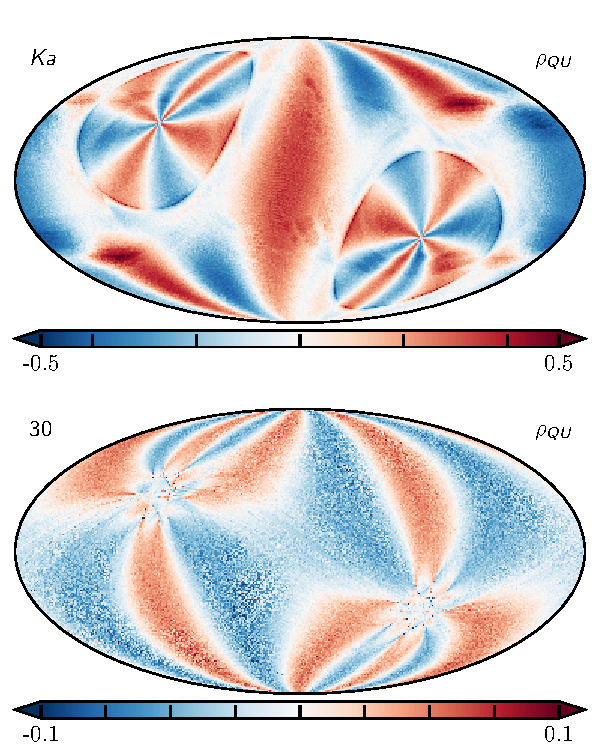
\includegraphics[width=\columnwidth]{figures/rho_QU.pdf}
%	\caption{$QU$ correlation for \WMAP\ \Ka-band \textit{(top)} and \Planck\ 30\,GHz \textit{(bottom)}. Note the differing dynamic range in the two maps.}
%	\label{fig:rho_qu}
%\end{figure}

%\subsection{Angular power spectra}



%\clearpage

%\section{High-level posterior distributions}
%\label{sec:maps}

\subsection{Astrophysical sky model}
\label{sec:skymodel}

\begin{figure}
	\centering
	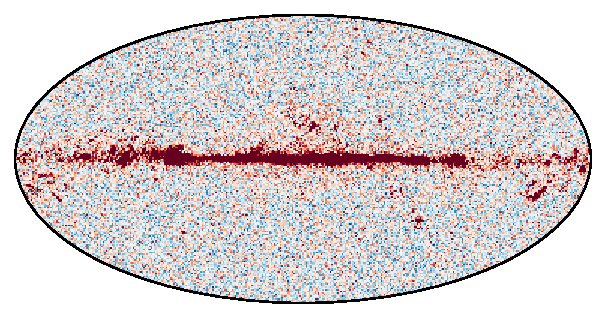
\includegraphics[width=\linewidth]{figures/chisq_IQU.pdf}
	\newline
	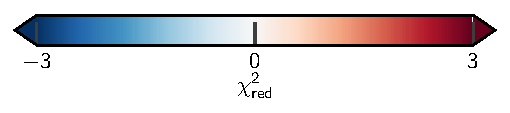
\includegraphics[width=0.3\textwidth]{figures/cbar_3sigma.pdf}
	\caption{Reduced-$\chi^2$, using $n_\mathrm{dof}=300$, which comes from fitting to the regions outside of the \K-band processing mask.}
\end{figure}


\section{Markov chains and parameter correlations}
\label{sec:traceplots}


\subsection{Trace plots}
\label{sec:traceplots}

\lipsum[1-4]


\subsection{Parameter correlations}
\label{sec:correlations}

\lipsum[5-8]

\subsubsection{\K-band calibration and AME}
\label{sec:kband_correlation}

In a preliminary \commanderthree\ run, we discovered an unbounded rise in the
\K-band absolute calibration, $g_0$, and the dipole in the AME component of the sky. Because the AME is strongest among all bands at \K-band, any increase in the \K-band absolute calibration can easily be accounted for by changing the amplitude of the AME, while leaving goodness-of-fit tests such as relative-$\chi^2$ and residual maps unaffected.

In order to break this degeneracy, it was necessary to impose a prior either on the AME itself or on the absolute calibration. The AME prior we explored followed the approach of \citet{bp13}, in which the prior mean was the \Planck\ DR4\,857 GHz map scaled by $3\cdot10^{-5}$, and the variance is given in angular scales by a parameter $q$. We found that a prior of $q=10^{-2}\,\mathrm{\mu K}^2$ was necessary to stabilize the gain, resulting in an AME map that was nearly identical to the \Planck\ 857\,GHz band. As this gave a result that was inconsistent with many previous results, we opted insted to sample the absolute calibration instead.

Any error in $g_0$ leads to a residual due to the large Solar dipole. In practice, we found that the typical variation of $g_0$ was 0.002, giving a relative error of $\sim0.1\,\%$. This variation induces a $\sim6\,\mathrm{\mu K}$ Solar dipole uncertainty, which is easily attributed to AME during component separation. In Figure \ref{fig:g0_ame}, we demonstrate this effect on recovered AME maps using extreme $g_0$ values of 1.175 and 1.9. We find that AME maps consistent with those presented in \citet{bennett2012} and \citet{planck2014-a12} are recovered when $g_0$ is between 1.180 and 1.182. Based on this analysis, we sample $g_0$ from a Gaussian with mean 1.1815 and standard deviation 0.001.

\citet{bennett2012} and \citet{planck2014-a12} find AME peak frequencies 12.0--17.5\,GHz and 17--23\,GHz, respectively, both with low signal-to-noise at high Galactic latitude and with structure along the plane. The Q-U-I JOint Tenerife Experiment (QUIJOTE) has recently released maps of the sky with approximately 70\,\% sky coverage at frequencies 11, 13, 17, and 19\,GHz \citep{QUIJOTE_IV}. QUIJOTE is optimized for characterizing the polarized sky, and constraints from, e.g., \citet{QUIJOTE_VIII}, will be critical for future polarized synchrotron SED characterization and polarized AME limits. While in principle the AME SED can be constrained by a joint \WMAP/LFI/QUIJOTE analysis, we consider this outside of the scope of the paper, which aims to evaluate the effect of jointly analyzing \WMAP\ and \Planck\ LFI at the TOD level.  Future analysis will include the QUIJOTE data, and hopefully break the $g_0$-$a_\mathrm{ame}$ degeneracy.

%\begin{figure}
%	\centering
%	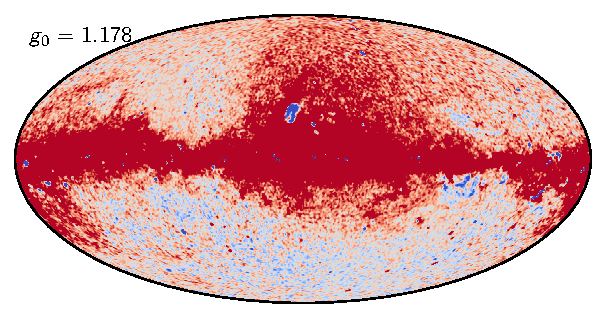
\includegraphics[width=\columnwidth]{figures/ame_g01_178.pdf}
%	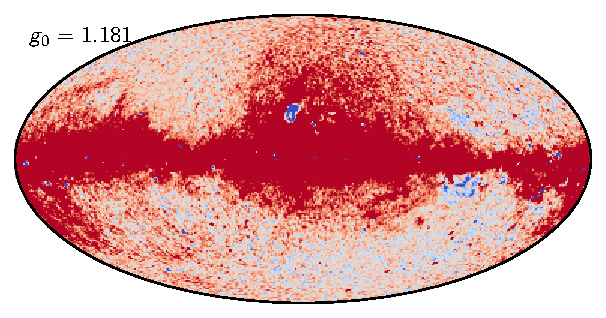
\includegraphics[width=\columnwidth]{figures/ame_g01_181.pdf}
%	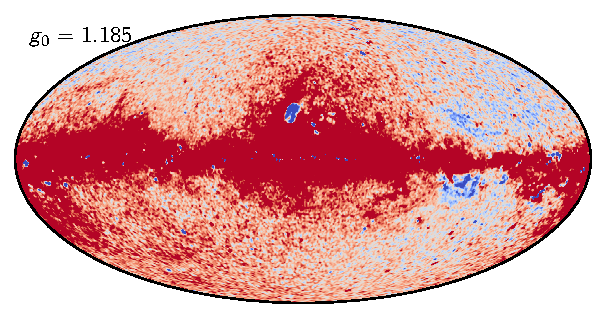
\includegraphics[width=\columnwidth]{figures/ame_g01_185.pdf}
%	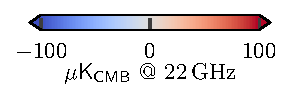
\includegraphics[width=0.5\columnwidth]{figures/cbar_100uK.pdf}
%	\caption{Dependence on AME amplitude evaluated at 22\,GHz as a function of absolute calibration. Each map comes from the fifth iteration of a dedicated \commander\ run that fixed $g_0$ while letting all other TOD parameters be fit. The values of $g_0=1.178$ and $g_0=1.185$ represent $3.5\sigma$ draws from the prior distribution with mean $1.1815$ and standard deviation $0.001$. The dipole visible in the top and bottom panels is aligned perfectly with the Solar dipole, and is directly due to variations in the \K-band absolute calibration.}
%	\label{fig:g0_ame}
%\end{figure}




These parameters are themselves sampled conditioned on a full sky model.

Remember that the frequency maps themselves are deterministic functions of the low-level sampled parameters.


%\subsection{Gain and baselines}

\lipsum[1-4]



%\subsection{Transmission imbalance}



%\subsection{Noise characterization}

\textit{The second main deviation\ldots} is in the treatment the noise power spectra. As shown
in Sect~2.5 of \citet{jarosik2007}, the noise autocorrelation spectrum is fit
on a year-by-year basis to a polynomial in $\log(\Delta t)$, where $\Delta t$
is the time lag between data points. This method is very similar to the
\commanderthree\ approach, which fits for the power spectrum in Fourier space
using a correlated noise model of the form
$\sigma_0^2(f/f_\mathrm{knee})^{\alpha}$. Properly parameterized, these two
approaches should yield similar results, albeit with different levels of
uncertainty and time resolution. However, we have confirmed that in many cases
the simple $1/f$ noise model does not fit the signal-subtracted TOD, yielding
$\chi^2$ values that are up to $10\sigma$ discrepant from their expected
values.  [Show, discuss figure with the PSDs, residual spectrum, and Bessel
filter.]

Deviations from the $1/f$ model consist either of a linear increase or downturn
above 10\,Hz. This can be partially explained by the use of a two pole Bessel
low-pass filter just prior to signal quantization, which introduces a 2.62\%
correlation between 25.6\,ms sample integrations
\citep[][Sect.~5.3]{jarosik2003:MAP}. The exact form of the Bessel filter was
not used on flight data, but rather the parametric fit as discussed above.
However, the filter is designed to reduce the signal by half at 100\,Hz, and as
such has a negligible effect. 




%\subsection{Goodness-of-fit}

\lipsum[1-4]

%\clearpage


\section{Frequency maps and astrophysical components}
\label{sec:maps}

\subsection{Map summary statistics}


\begin{figure*}
	\centering
	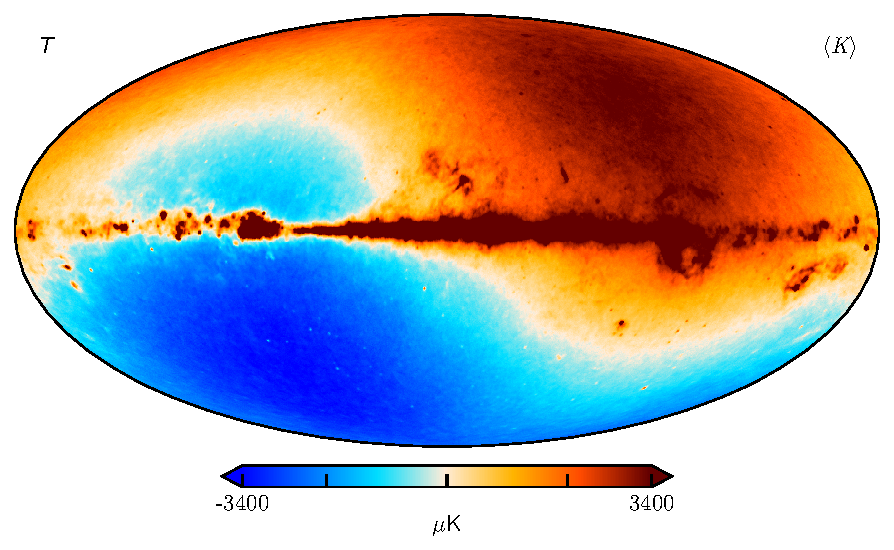
\includegraphics[width=0.75\textwidth]{figures/023-WMAP_K_mu_I.pdf}
	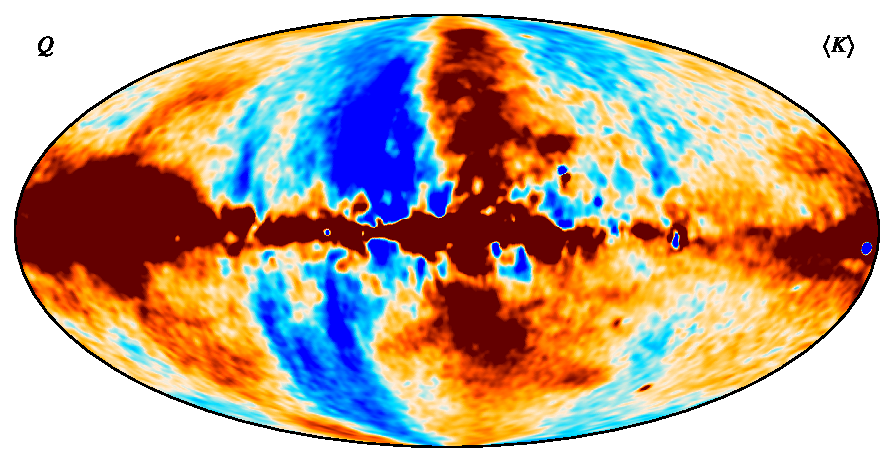
\includegraphics[width=0.75\textwidth]{figures/023-WMAP_K_mu_Q.pdf}
	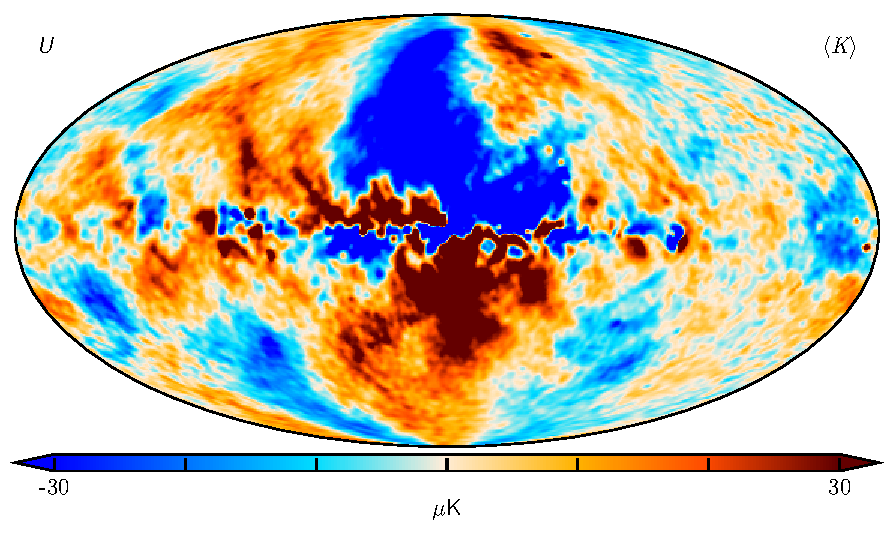
\includegraphics[width=0.75\textwidth]{figures/023-WMAP_K_mu_U.pdf}
	\caption{\K-band}
\end{figure*}
\begin{figure*}
	\centering
	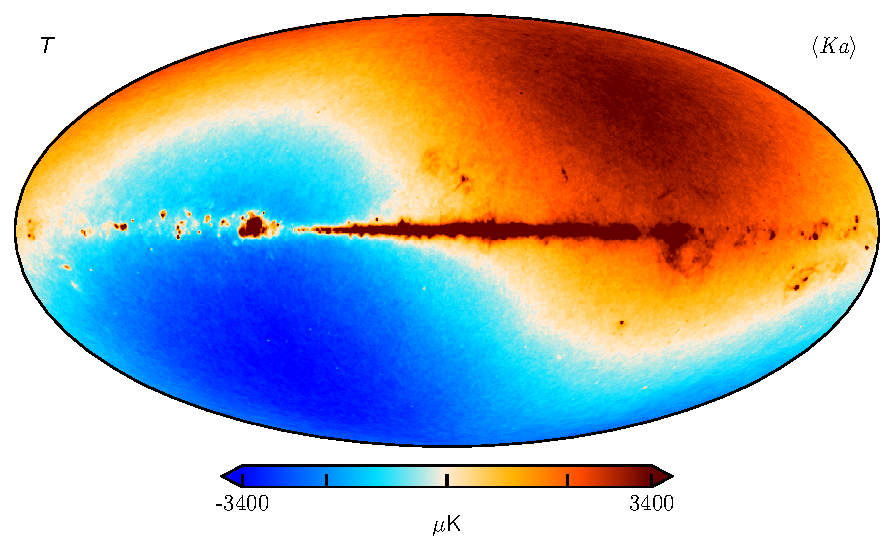
\includegraphics[width=0.75\textwidth]{figures/030-WMAP_Ka_mu_I.pdf}
	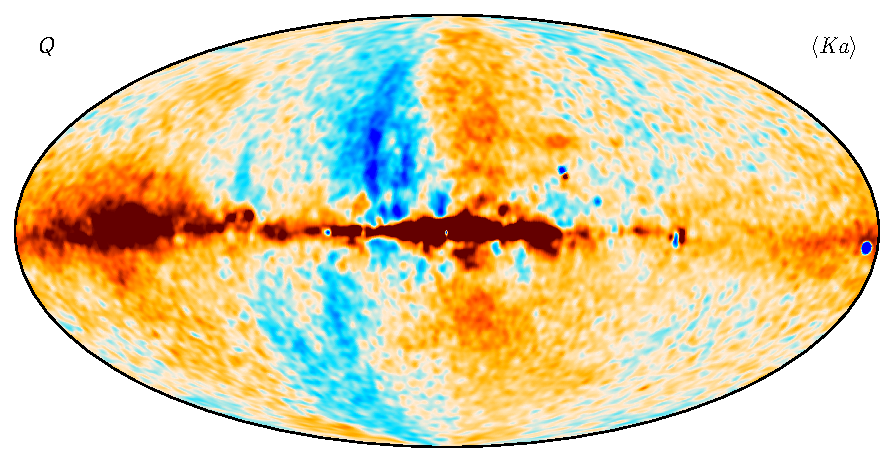
\includegraphics[width=0.75\textwidth]{figures/030-WMAP_Ka_mu_Q.pdf}
	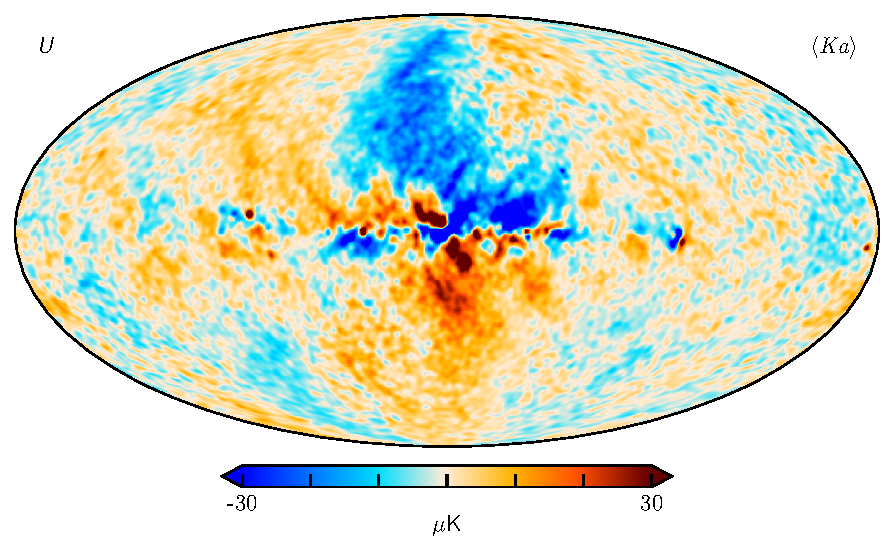
\includegraphics[width=0.75\textwidth]{figures/030-WMAP_Ka_mu_U.pdf}
	\caption{\Ka-band}
\end{figure*}
\begin{figure*}
	\centering
	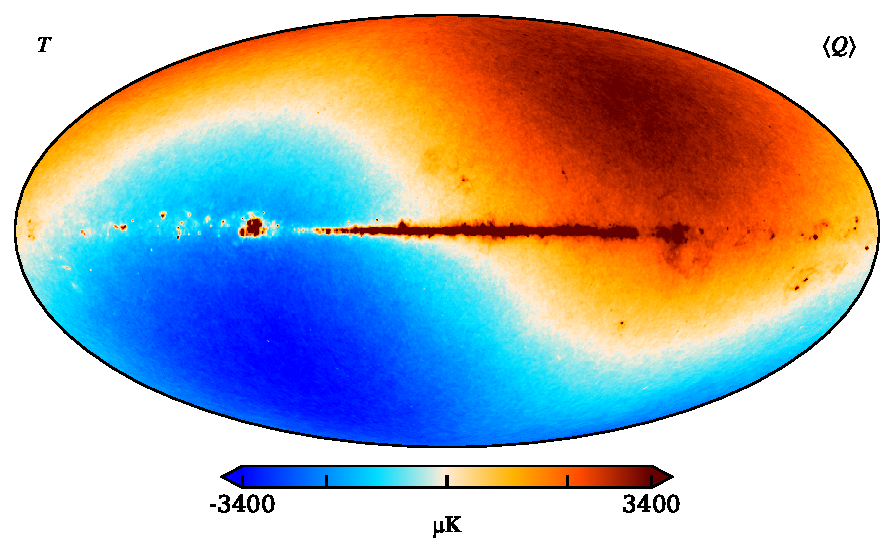
\includegraphics[width=0.75\textwidth]{figures/Q_mu_I.pdf}
	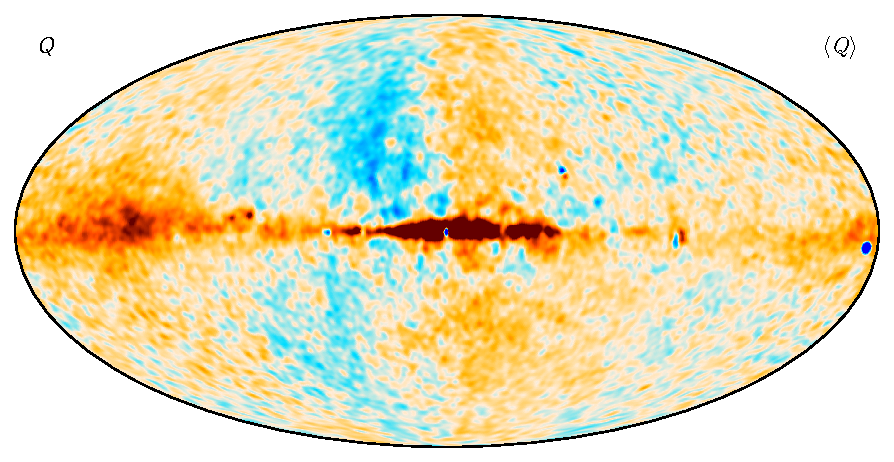
\includegraphics[width=0.75\textwidth]{figures/Q_mu_Q.pdf}
	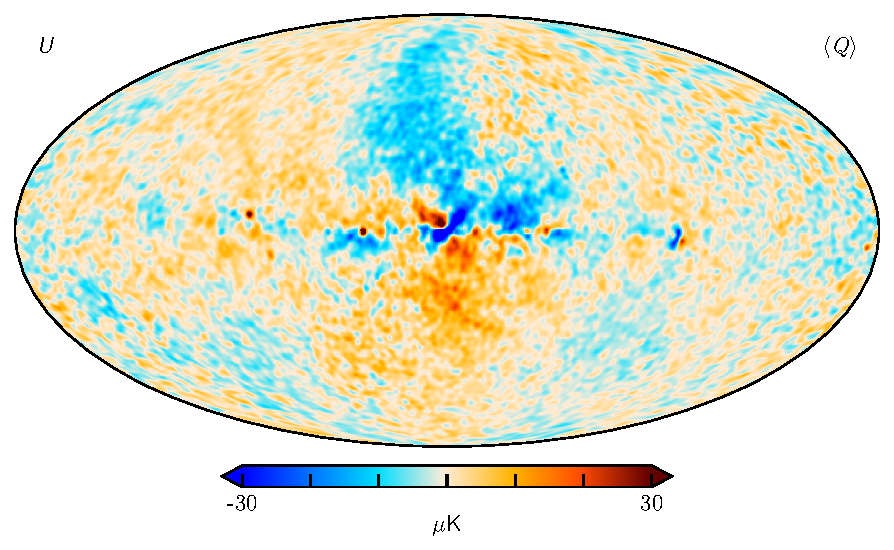
\includegraphics[width=0.75\textwidth]{figures/Q_mu_U.pdf}
	\caption{\Q-band}
\end{figure*}
\begin{figure*}
	\centering
	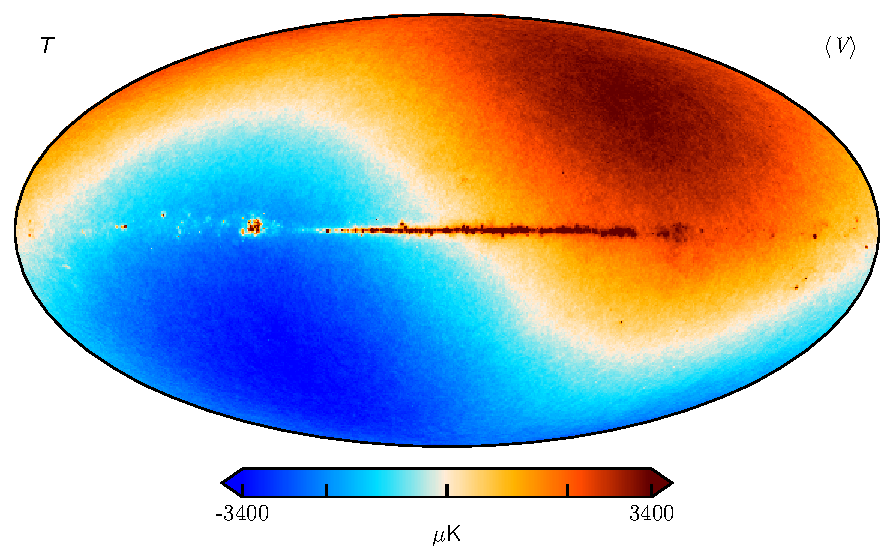
\includegraphics[width=0.75\textwidth]{figures/V_mu_I.pdf}
	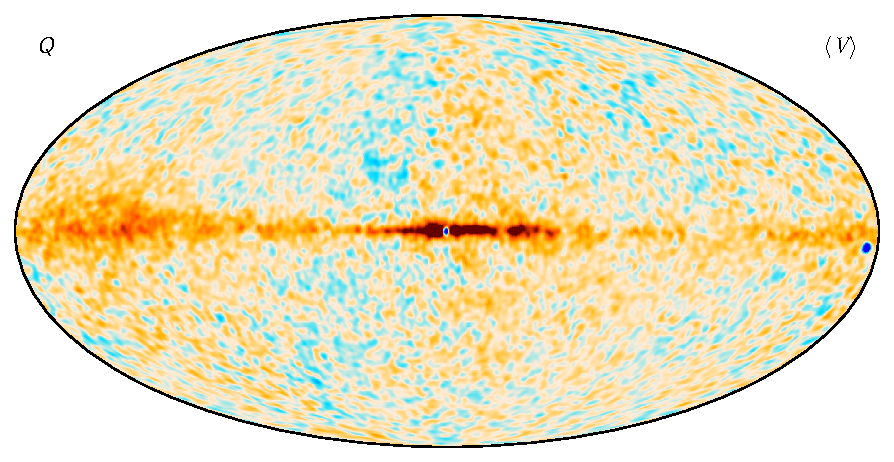
\includegraphics[width=0.75\textwidth]{figures/V_mu_Q.pdf}
	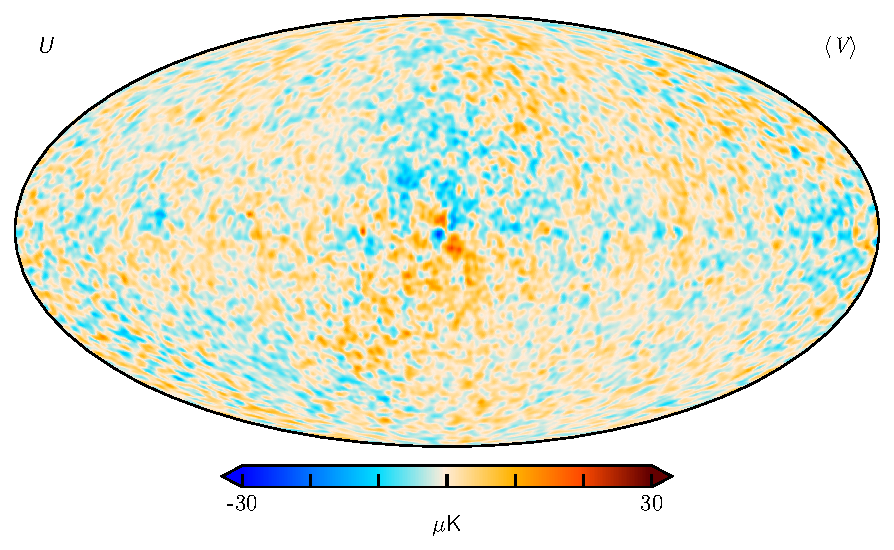
\includegraphics[width=0.75\textwidth]{figures/V_mu_U.pdf}
	\caption{\V-band}
\end{figure*}
\begin{figure*}
	\centering
	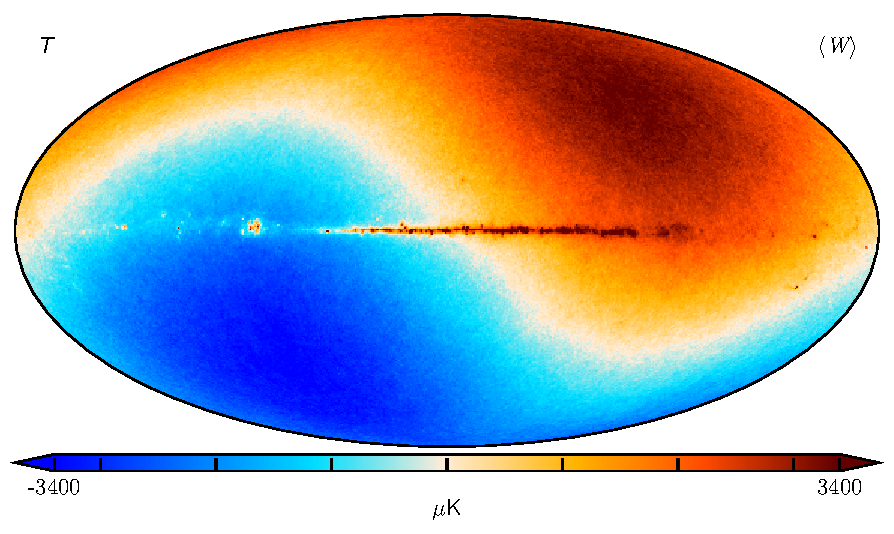
\includegraphics[width=0.75\textwidth]{figures/W_mu_I.pdf}
	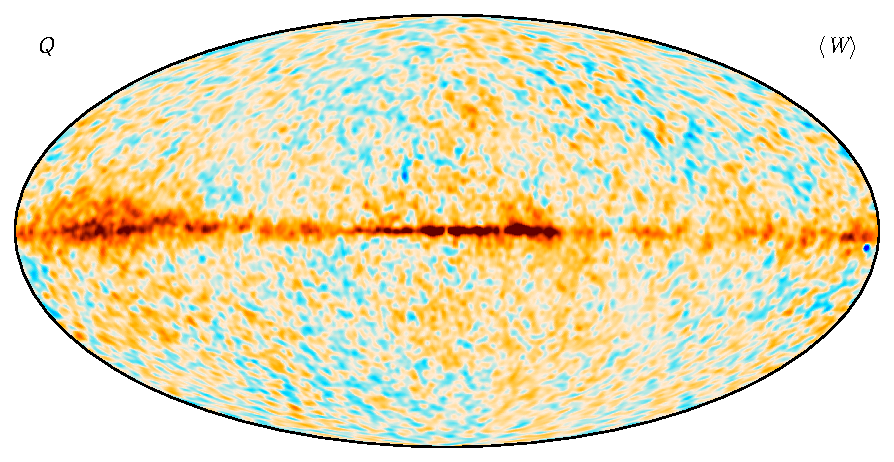
\includegraphics[width=0.75\textwidth]{figures/W_mu_Q.pdf}
	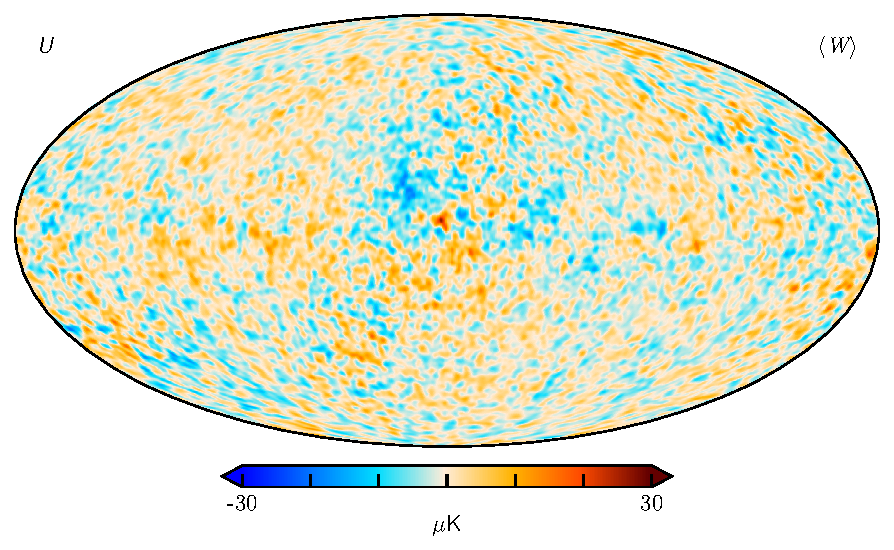
\includegraphics[width=0.75\textwidth]{figures/W_mu_U.pdf}
	\caption{\W-band}
\end{figure*}


%\subsection{Posterior uncertainties}

\begin{figure*}[t]
	\centering
	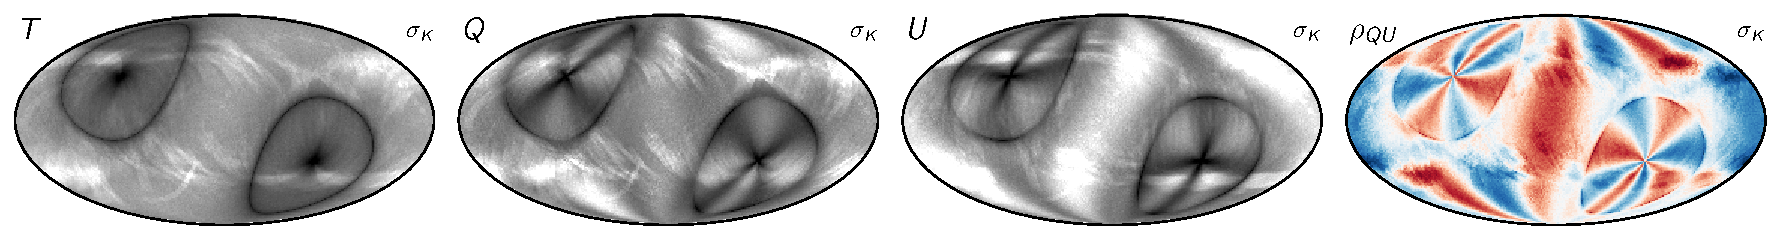
\includegraphics[width=\textwidth]{figures/023-WMAP_K_rms.pdf}\\
	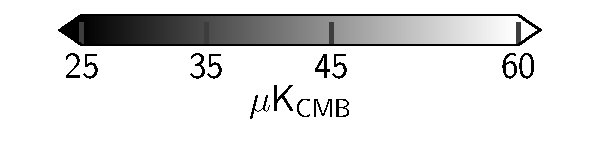
\includegraphics[width=0.22\textwidth]{figures/cbar_rms_I.pdf}
	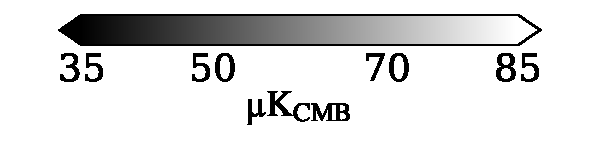
\includegraphics[width=0.22\textwidth]{figures/cbar_rms_P.pdf}
	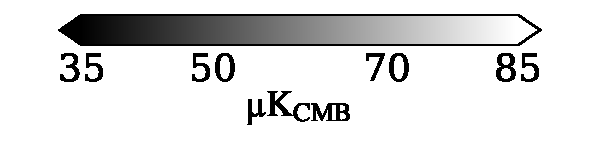
\includegraphics[width=0.22\textwidth]{figures/cbar_rms_P.pdf}
	\includegraphics[width=0.22\textwidth]{figures/cbar_rho.pdf}
	\caption{RMS}
        \label{fig:Krms}
\end{figure*}

\begin{figure*}[t]
	\centering
	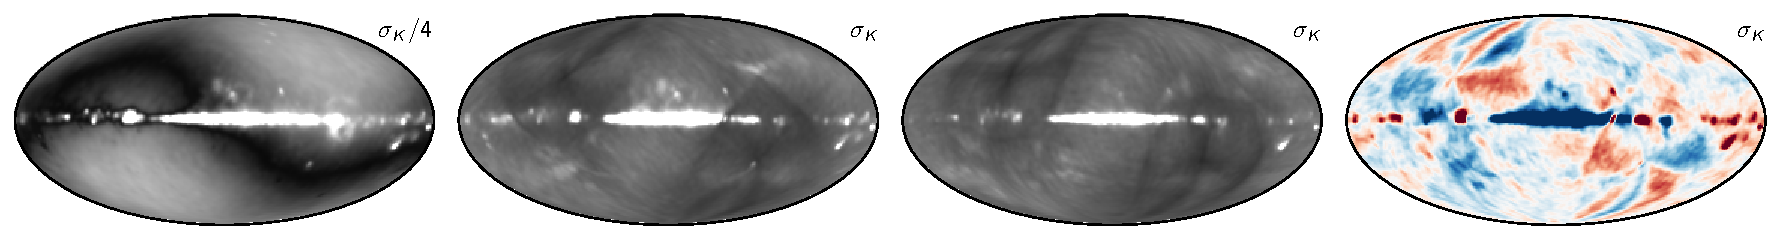
\includegraphics[width=\textwidth]{figures/023-WMAP_K_std.pdf}\\
	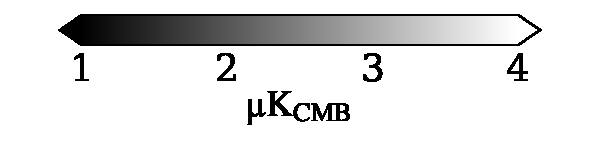
\includegraphics[width=0.22\textwidth]{figures/cbar_std.pdf}
	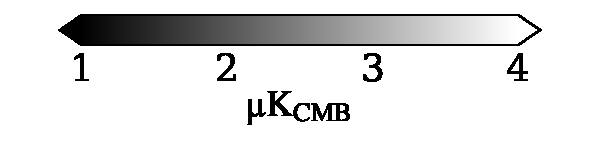
\includegraphics[width=0.22\textwidth]{figures/cbar_std.pdf}
	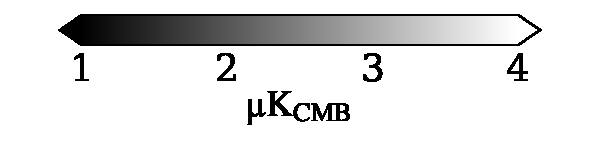
\includegraphics[width=0.22\textwidth]{figures/cbar_std.pdf}
	\includegraphics[width=0.22\textwidth]{figures/cbar_rho.pdf}\\
	\caption{Kstd}
        \label{fig:Kstd}
\end{figure*}

\begin{figure*}[t]
	\centering
	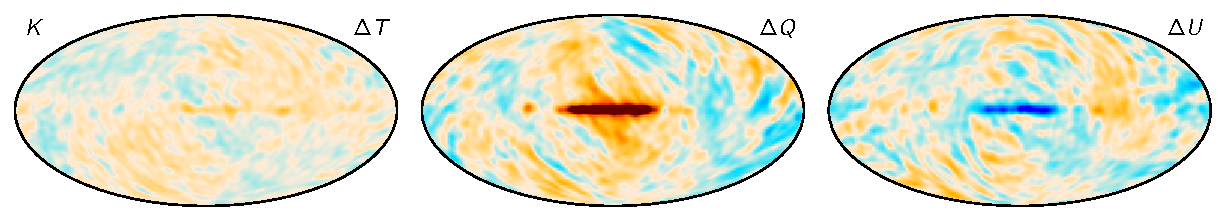
\includegraphics[width=\textwidth]{figures/023-WMAP_K_sampdiff.pdf}\\
	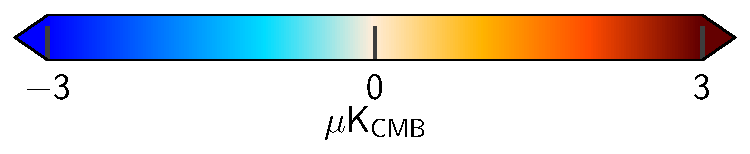
\includegraphics[width=0.30\textwidth]{figures/cbar_3uK.pdf}        
	\caption{K sample diff}
        \label{fig:Ksampdiff}
\end{figure*}

\begin{figure*}[t]
	\centering
	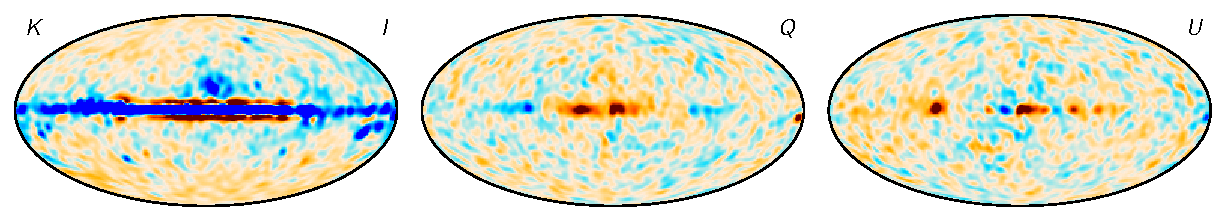
\includegraphics[width=\textwidth]{figures/res_K_IQU.pdf}\\
	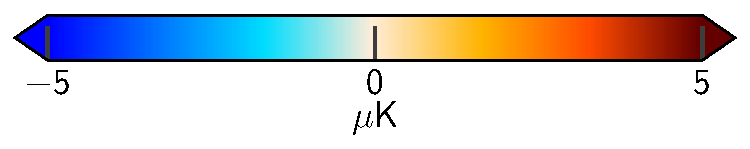
\includegraphics[width=0.30\textwidth]{figures/cbar_5uK.pdf}        
	\caption{K residual}
        \label{fig:Kres}
\end{figure*}

\begin{figure*}[t]
	\centering
	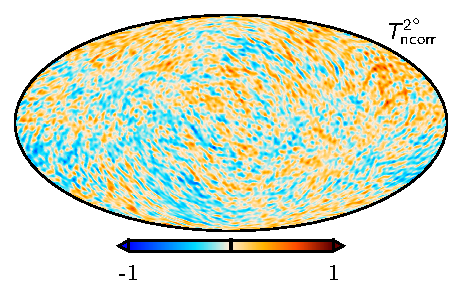
\includegraphics[width=0.32\textwidth]{figures/K_ncorr_I.pdf}
	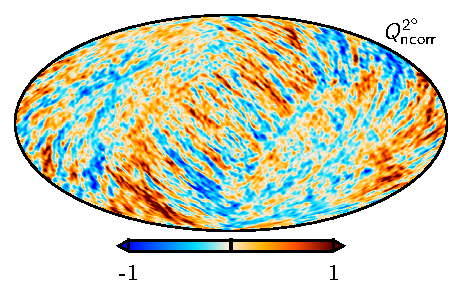
\includegraphics[width=0.32\textwidth]{figures/K_ncorr_Q.pdf}
	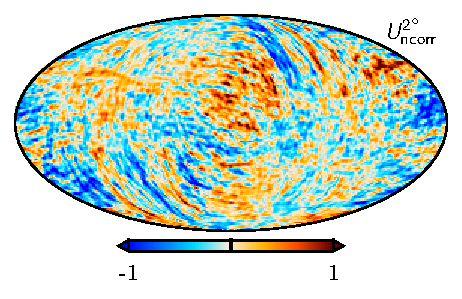
\includegraphics[width=0.32\textwidth]{figures/K_ncorr_U.pdf}\\
	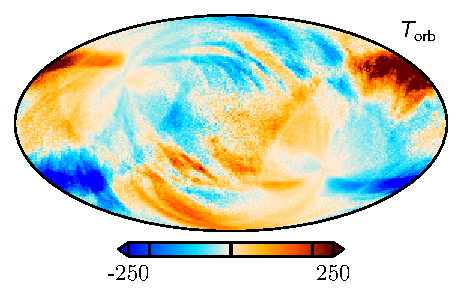
\includegraphics[width=0.32\textwidth]{figures/K_orb_I.pdf}
	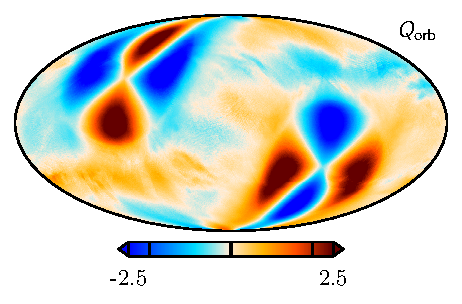
\includegraphics[width=0.32\textwidth]{figures/K_orb_Q.pdf}
	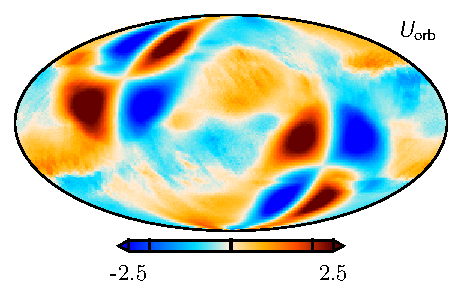
\includegraphics[width=0.32\textwidth]{figures/K_orb_U.pdf}\\
	\includegraphics[width=0.32\textwidth]{figures/K_leak_I.pdf}
	\includegraphics[width=0.32\textwidth]{figures/K_leak_Q.pdf}
	\includegraphics[width=0.32\textwidth]{figures/K_leak_U.pdf}\\
	\includegraphics[width=0.32\textwidth]{figures/K_sl_I.pdf}
	\includegraphics[width=0.32\textwidth]{figures/K_sl_Q.pdf}
	\includegraphics[width=0.32\textwidth]{figures/K_sl_U.pdf}\\
	\includegraphics[width=0.32\textwidth]{figures/K_res_I.pdf}
	\includegraphics[width=0.32\textwidth]{figures/K_res_Q.pdf}
	\includegraphics[width=0.32\textwidth]{figures/K_res_U.pdf}\\
	\caption{Time-ordered components projected}
\end{figure*}



\begin{figure*}
	\centering
	\includegraphics[width=0.32\textwidth]{figures/megadiff_K_I.pdf}
        \includegraphics[width=0.32\textwidth]{figures/megadiff_K_Q.pdf}
        \includegraphics[width=0.32\textwidth]{figures/megadiff_K_U.pdf}\\\vspace*{-4mm}
	\includegraphics[width=0.32\textwidth]{figures/megadiff_Ka_I.pdf}
        \includegraphics[width=0.32\textwidth]{figures/megadiff_Ka_Q.pdf}
        \includegraphics[width=0.32\textwidth]{figures/megadiff_Ka_U.pdf}\\\vspace*{-4mm}
	\includegraphics[width=0.32\textwidth]{figures/megadiff_Q_I.pdf}
        \includegraphics[width=0.32\textwidth]{figures/megadiff_Q_Q.pdf}
        \includegraphics[width=0.32\textwidth]{figures/megadiff_Q_U.pdf}\\\vspace*{-4mm}
	\includegraphics[width=0.32\textwidth]{figures/megadiff_V_I.pdf}
        \includegraphics[width=0.32\textwidth]{figures/megadiff_V_Q.pdf}
        \includegraphics[width=0.32\textwidth]{figures/megadiff_V_U.pdf}\\\vspace*{-4mm}
	\includegraphics[width=0.32\textwidth]{figures/megadiff_W_I.pdf}
        \includegraphics[width=0.32\textwidth]{figures/megadiff_W_Q.pdf}
        \includegraphics[width=0.32\textwidth]{figures/megadiff_W_U.pdf}\\\vspace*{-4mm}
	\includegraphics[width=0.8\textwidth]{figures/cbar_10uK_symlog2.pdf}
	\caption{Difference maps between the \cosmoglobe\ and 9-year \WMAP\ frequency maps. Columns show Stokes $T$, $Q$, and $U$ parameter maps, while rows show $K$-, $Ka$-, $Q$-, $V$-, and $W$-band maps. The temperature maps are smoothed to an angular resolution of $1^{\circ}$ FWHM, while the polarization maps are smoothed to $5^{\circ}$ FWHM.}
        \label{fig:megadiff_wmap}
\end{figure*}


%\subsection{Angular power spectra}

Will combine these spectra shortly

\begin{figure*}
	\centering
	\includegraphics[width=0.8\textwidth]{figures/TT_spectra.pdf}
	\caption{TT power spectra}
\end{figure*}
\begin{figure*}
	\centering
	\includegraphics[width=0.8\textwidth]{figures/EE_spectra.pdf}
	\caption{EE power spectra}
\end{figure*}
\begin{figure*}
	\centering
	\includegraphics[width=0.8\textwidth]{figures/BB_spectra.pdf}
	\caption{BB power spectra}
\end{figure*}
%\begin{figure*}
%	\centering
%	\includegraphics[width=0.8\textwidth]{figures/TT_spectra_zoom.pdf}
%	\caption{TT power spectra zoom}
%\end{figure*}
%\begin{figure*}
%	\centering
%	\includegraphics[width=0.8\textwidth]{figures/EE_spectra_zoom.pdf}
%	\caption{EE power spectra zoom}
%\end{figure*}
%\begin{figure*}
%	\centering
%	\includegraphics[width=0.8\textwidth]{figures/BB_spectra_zoom.pdf}
%	\caption{BB power spectra zoom}
%\end{figure*}
\begin{figure*}
	\centering
	\includegraphics[width=0.8\textwidth]{figures/TT_spectra_ratio.pdf}
	\caption{TT ratios}
\end{figure*}
\begin{figure*}
	\centering
	\includegraphics[width=0.8\textwidth]{figures/EE_spectra_ratio.pdf}
	\caption{EE ratios}
\end{figure*}
\begin{figure*}
	\centering
	\includegraphics[width=0.8\textwidth]{figures/BB_spectra_ratio.pdf}
	\caption{BB ratios}
\end{figure*}


%\section{Preliminary astrophysical results}
%\subsection{Diffuse foregrounds}
%\subsection{CMB constraints}
%\subsubsection{Solar dipole}
%\subsubsection{Temperature power spectrum}


%\clearpage


Want to compare the $QU$ correlation in WMAP and Planck LFI, get a quantitative number. Point out that the polarization solution itself is much better, but the covariance between pixels themselves is much higher. This wasn't an issue for LFI, so we had to take that into account here.

I also want to put a bit here on why the low-$\ell$ approach needed to be done separately, how correlated noise sampling addresses it, to what extent it's mitigated, etc.

Note that LFI's 30 and 70\,GHz $QU$ correlation is $\sim0.1$, whereas 44\,GHz is much larger, $\sim0.5$. This discrepancy is due to the number of horns with differing polarization orientation. Both 30 and 70\,GHz have an even number of horns, allowing for pairs of datastreams to be combined to give independent polarization measurements. Conversely, 44\,GHz has one horn pair and an unpaired horn, the latter of which induces more correlation in the $QU$ observation matrix. An example for \Ka\ and 30\,GHz is shown in Fig.~\ref{fig:rho_qu}. Aside from the obvious morphological changes due to the two experiments' different observing strategies, the magnitude of \WMAP's correlation is much larger than \Planck's.

The \BP\ project took this covariance structure into account using the dense $N_\mathrm{side}=16$ noise covariance matrix provided by the \WMAP\ team.\footnote{\url{https://lambda.gsfc.nasa.gov/product/wmap/dr5/ninv_info.html}} Properly sampled correlated noise only leaves white nosie in the maps, so the noise properties of each map's sample do not require a dense pixel-pixel covariance, even at low resolution \citep{bp01, bp10}. 
The \WMAPnine\ inverse noise covariance matrices were computed using the full time-space noise matrix $\mathsf N=\mathsf N^\mathrm w+\mathsf N^\mathrm{corr}$, so the full pixel-pixel covariance matrix $\Sigma^{-1}=\mathsf P^T\mathsf N^{-1}\mathsf P$ took into account the correlation between neighboring samples. The \cosmoglobe\ maps, by subtracting a realization of correlated noise before mapmaking, estimates an inerse noise covariance matrix
\begin{equation}
	\Sigma^{-1}_{pp'}
	=\sum_{t_1,t_2}\mathsf P_{t_1,p_1}^T\mathsf N_{t_1,t_2}^{-1}\mathsf P_{t_2,p_2}
	=\sum_t\mathsf P_{t,p_1}^T\mathsf N_{t,t}^{-1}\mathsf P_{t,p_2}
\end{equation}

How much off-diagonal pixel covariance is there here?

dense noise covariance matrix also explicitly projected out the poorly-measured imbalance modes, but because we find no trace of these modes in our sky maps or residual maps, this treatment is not necessary in our approach. However, the correlation between Stokes $Q$ and $U$ was not taken into account in the \BP\ LFI analysis. This was not a significant oversight in the LFI analysis because the 30 and 70\,GHz maps only had a 10\% correlation, and 44\,GHz's 50\% correlation was subdominant to other systematic effects. We have updated \commanderthree\ to take $QU$ correlation into account for LFI.


\subsection{Comparison with 9-year \WMAP\ maps}
\label{sec:wmap_comparison}

\begin{table}
\newdimen\tblskip \tblskip=5pt
\caption{Difference map $\chi^2$ statistics.  }
\label{tab:chisq}
\vskip -4mm
\footnotesize
\setbox\tablebox=\vbox{
 \newdimen\digitwidth
 \setbox0=\hbox{\rm 0}
 \digitwidth=\wd0
 \catcode`*=\active
 \def*{\kern\digitwidth}
%
  \newdimen\dpwidth
  \setbox0=\hbox{.}
  \dpwidth=\wd0
  \catcode`!=\active
  \def!{\kern\dpwidth}
%
  \halign{\hbox to 2.5cm{#\leaderfil}\tabskip 2em&
    \hfil$#$\hfil \tabskip 2em&
    \hfil$#$\hfil \tabskip 2em&    
    \hfil$#$\hfil \tabskip 0em\cr
\noalign{\doubleline}
\omit\hfil\sc Difference \hfil& \chi^2_{\mathrm{uncorr}} & \chi^2_{\mathrm{corr}} & \Delta \chi^2\cr
\noalign{\vskip 3pt\hrule\vskip 5pt}
$0.32\times$K1 $-$ Ka1  & 4291  & 4287  & **4 \cr
Q1 $-$ Q2         & 4500  & 4380  & 120 \cr
V1 $-$ V2         & 4490  & 4429  & *61 \cr
W1 $-$ W2         & 4328  & 4270  & *68 \cr
W3 $-$ W4         & 4257  & 4145  & 112 \cr
\noalign{\vskip 5pt\hrule\vskip 5pt}}}
\endPlancktablewide
\end{table}


\begin{table}
\newdimen\tblskip \tblskip=5pt
\caption{Transmission imbalance template amplitudes for each \WMAP\ radiometer as estimated by fitting the official templates to low-resolution difference maps between \cosmoglobe\ and \WMAP. The templates are provided in mK, and the template amplitudes are therefore dimensionless. The fourth column lists the relative decrease in standard deviation, $\sqrt{\sigma_{\mathrm{raw}}^2 - \sigma_{\mathrm{corr}}^2}/\sigma_{\mathrm{raw}}$,  after subtracting the best-fit templates in percent. }
\label{tab:transmission}
\vskip -4mm
\footnotesize
\setbox\tablebox=\vbox{
 \newdimen\digitwidth
 \setbox0=\hbox{\rm 0}
 \digitwidth=\wd0
 \catcode`*=\active
 \def*{\kern\digitwidth}
%
  \newdimen\dpwidth
  \setbox0=\hbox{.}
  \dpwidth=\wd0
  \catcode`!=\active
  \def!{\kern\dpwidth}
%
  \halign{\hbox to 1.8cm{#\leaderfil}\tabskip 2em&
    \hfil$#$\hfil \tabskip 2em&
    \hfil$#$\hfil \tabskip 2em&    
    \hfil$#$\hfil \tabskip 0em\cr
\noalign{\doubleline}
\omit\hfil\sc DA \hfil& a_1 & a_2 & \Delta \sigma [\%]\cr
\noalign{\vskip 3pt\hrule\vskip 5pt}
K1 &   -27.5*  &  -50.6* & 30 \cr
Ka1 &   -1.4  &   -1.9 & 25 \cr
Q1 &   -30.0* &  -71.6* & 11 \cr
Q2 &   -7.1  &  -1.5 & 20 \cr
V1 &   -32.8*  &  -53.4* & *6 \cr
V2 &   *8.8  &  -4.1 & 16 \cr
W1 &   -2.8  &  *4.6 & *8 \cr
W2 &   -6.9  & -3.5 & 11 \cr
W3 &   29.1  & 53.4 & 12 \cr
W4 &   15.5  & -6.8 & 52 \cr
\noalign{\vskip 5pt\hrule\vskip 5pt}}}
\endPlancktablewide
\end{table}



\begin{figure}[t]
  \centering
  \includegraphics[width=\linewidth]{figures/diff_K1_Q.pdf}\\
  \includegraphics[width=\linewidth]{figures/temp_corr_K1_Q.pdf}\\
  \includegraphics[width=\linewidth]{figures/res_loss_K1_Q.pdf}
  \caption{K-band transmission imbalance templates}
  \label{fig:Kimbal}
\end{figure}


\subsection{Consistency within \WMAP\ channels}
\label{sec:internal_consistency}

\begin{figure*}
	\centering
	%\includegraphics[width=0.24\textwidth]{figures/K30_deltaQ.pdf}
	%\includegraphics[width=0.24\textwidth]{figures/K30_W_deltaQ.pdf}
	%\includegraphics[width=0.24\textwidth]{figures/K30_deltaU.pdf}
	%\includegraphics[width=0.24\textwidth]{figures/K30_W_deltaU.pdf}
	%\includegraphics[width=0.24\textwidth]{figures/30Ka_deltaQ.pdf}
	%\includegraphics[width=0.24\textwidth]{figures/30Ka_W_deltaQ.pdf}
	%\includegraphics[width=0.24\textwidth]{figures/30Ka_deltaU.pdf}
	%\includegraphics[width=0.24\textwidth]{figures/30Ka_W_deltaU.pdf}
	\includegraphics[width=0.24\textwidth]{figures/KKa_deltaQ.pdf}
	\includegraphics[width=0.24\textwidth]{figures/KKa_W_deltaQ.pdf}
	\includegraphics[width=0.24\textwidth]{figures/KKa_deltaU.pdf}
	\includegraphics[width=0.24\textwidth]{figures/KKa_W_deltaU.pdf}\\
	\includegraphics[width=0.24\textwidth]{figures/Q_deltaQ.pdf}
	\includegraphics[width=0.24\textwidth]{figures/Q_W_deltaQ.pdf}
	\includegraphics[width=0.24\textwidth]{figures/Q_deltaU.pdf}
	\includegraphics[width=0.24\textwidth]{figures/Q_W_deltaU.pdf}\\
	\includegraphics[width=0.24\textwidth]{figures/V_deltaQ.pdf}
	\includegraphics[width=0.24\textwidth]{figures/V_W_deltaQ.pdf}
	\includegraphics[width=0.24\textwidth]{figures/V_deltaU.pdf}
	\includegraphics[width=0.24\textwidth]{figures/V_W_deltaU.pdf}\\
	\includegraphics[width=0.24\textwidth]{figures/W_deltaQ.pdf}
	\includegraphics[width=0.24\textwidth]{figures/W_W_deltaQ.pdf}
	\includegraphics[width=0.24\textwidth]{figures/W_deltaU.pdf}
	\includegraphics[width=0.24\textwidth]{figures/W_W_deltaU.pdf}
	\caption{Half-difference maps, smoothed by $10^\circ$.}
\end{figure*}


\begin{figure}
	\centering
	\includegraphics[width=\linewidth]{figures/cls_cg_WMAP_lowl.pdf}
	\caption{Half-difference spectra.}
        \label{fig:cl_halfdiff}
\end{figure}



\subsection{Consistency between \WMAP\ and LFI}
\label{sec:lfi_consistency}

\begin{figure*}
	\centering
	\includegraphics[width=0.24\textwidth]{figures/K30_deltaQ.pdf}
	\includegraphics[width=0.24\textwidth]{figures/K30_W_deltaQ.pdf}
	\includegraphics[width=0.24\textwidth]{figures/K30_deltaU.pdf}
	\includegraphics[width=0.24\textwidth]{figures/K30_W_deltaU.pdf}
	\includegraphics[width=0.24\textwidth]{figures/30Ka_deltaQ.pdf}
	\includegraphics[width=0.24\textwidth]{figures/30Ka_W_deltaQ.pdf}
	\includegraphics[width=0.24\textwidth]{figures/30Ka_deltaU.pdf}
	\includegraphics[width=0.24\textwidth]{figures/30Ka_W_deltaU.pdf}
        \includegraphics[width=0.25\textwidth]{figures/cbar_10uK.pdf}
	\caption{Mean of \textit{WMAP}+LFI bands}
\end{figure*}


%\begin{figure*}
%	\centering
%	%\includegraphics[width=0.93\linewidth]{figures/megadiff.pdf}
%	\includegraphics[width=0.24\textwidth]{figures/megadiff_K_I.pdf}
%	\includegraphics[width=0.24\textwidth]{figures/megadiff_K_Q.pdf}
%	\includegraphics[width=0.24\textwidth]{figures/megadiff_K_U.pdf}\\
%	\includegraphics[width=0.24\textwidth]{figures/megadiff_030_I.pdf}
%	\includegraphics[width=0.24\textwidth]{figures/megadiff_030_Q.pdf}
%	\includegraphics[width=0.24\textwidth]{figures/megadiff_030_U.pdf}\\
%	\includegraphics[width=0.24\textwidth]{figures/megadiff_Ka_I.pdf}
%	\includegraphics[width=0.24\textwidth]{figures/megadiff_Ka_Q.pdf}
%	\includegraphics[width=0.24\textwidth]{figures/megadiff_Ka_U.pdf}\\
%	\includegraphics[width=0.24\textwidth]{figures/megadiff_044_I.pdf}
%	\includegraphics[width=0.24\textwidth]{figures/megadiff_044_Q.pdf}
%	\includegraphics[width=0.24\textwidth]{figures/megadiff_044_U.pdf}\\
%	\includegraphics[width=0.24\textwidth]{figures/megadiff_Q_I.pdf}
%	\includegraphics[width=0.24\textwidth]{figures/megadiff_Q_Q.pdf}
%	\includegraphics[width=0.24\textwidth]{figures/megadiff_Q_U.pdf}\\
%	\includegraphics[width=0.24\textwidth]{figures/megadiff_V_I.pdf}
%	\includegraphics[width=0.24\textwidth]{figures/megadiff_V_Q.pdf}
%	\includegraphics[width=0.24\textwidth]{figures/megadiff_V_U.pdf}\\
%	\includegraphics[width=0.24\textwidth]{figures/megadiff_070_I.pdf}
%	\includegraphics[width=0.24\textwidth]{figures/megadiff_070_Q.pdf}
%	\includegraphics[width=0.24\textwidth]{figures/megadiff_070_U.pdf}\\
%	\includegraphics[width=0.24\textwidth]{figures/megadiff_W_I.pdf}
%	\includegraphics[width=0.24\textwidth]{figures/megadiff_W_Q.pdf}
%	\includegraphics[width=0.24\textwidth]{figures/megadiff_W_U.pdf}\\
%	\includegraphics[width=0.5\textwidth]{figures/cbar_10uK_symlog2.pdf}
%	\caption{Differences between Commander-processed chains and official maps (BP10 and WMAP9)}
%\end{figure*}


\subsection{Preliminary CMB results}
\label{sec:cmb}

\subsubsection{CMB Solar dipole}
\label{sec:dipole}

\subsubsection{Temperature power spectrum}
\label{sec:cls}

\subsubsection{Preliminary large-scale CMB polarization results}
\label{sec:lowl_cmb}


\begin{figure}[t]
  \centering
        \includegraphics[width=0.49\linewidth]{figures/wtr39yrKaQVmapq.pdf}
        \includegraphics[width=0.49\linewidth]{figures/wtr39yrKaQVmapu.pdf}\\
        \includegraphics[width=0.49\linewidth]{figures/wmap_reprod_KaQV_9yr_q_scale.pdf}
        \includegraphics[width=0.49\linewidth]{figures/wmap_reprod_KaQV_9yr_u_scale.pdf}\\
        \includegraphics[width=0.49\linewidth]{figures/wmap_reprod_tempcorr_KaQV_9yr_q_scale.pdf}
        \includegraphics[width=0.49\linewidth]{figures/wmap_reprod_tempcorr_KaQV_9yr_u_scale.pdf}
	\caption{Noise-weighted likelihood input maps.}
	\label{fig:likelihood_maps}
\end{figure}


\begin{figure}[t]
  	\centering
	\includegraphics[width=\linewidth]{figures/lnL_EE_v1.pdf}
        \includegraphics[width=\linewidth]{figures/lnL_BB_v1.pdf}
	\caption{Likelihood slices}
	\label{fig:lnL}
\end{figure}


\subsection{Signal-to-noise ratio comparison between \WMAP\ and LFI}
\label{sec:s2n}


\begin{figure}
  \center	
  \includegraphics[width=\linewidth]{figures/fg_s2n_v1.pdf}
  \caption{Relative signal-to-noise ratios for WMAP and LFI channels and various components. }
  \label{fig:fg_s2n}
\end{figure}




%\clearpage
\section{Systematic error corrections and uncertainties}
\label{sec:systematics}

\subsection{Sky map corrections}



\subsection{Power spectrum residuals}

\begin{figure*}
  \center	
  \includegraphics[width=0.98\linewidth]{figures/components_power_spectrum_std_masked.pdf}
  \caption{Pseudo-spectrum standard deviation for each instrumental
    systematic correction shown in
    Figs.~\ref{fig:corrmaps30}--\ref{fig:corrmaps70} (\emph{thin
      colored lines}). For comparison, thick black lines show spectra
    for the full coadded frequency map; thick red lines show the
    standard deviation of the same (i.e., the full systematic
    uncertainty); gray lines show white noise; and dashed black lines
    show the best-fit \Planck\ 2018 $\Lambda$CDM power spectrum
    convolved with the instrument beam. Columns show results for 30,
    44 and 70\,GHz, respectively, while rows show results for each of
    the six polarization states ($TT$, $EE$, $BB$, $TE$, $TB$, and
    $EB$). All spectra have been derived outside the CMB confidence
    mask presented by \citet{bp13} using the HEALPix \texttt{anafast}
    utility, correcting only for sky fraction and not for mask mode
    coupling. }
  \label{fig:corrmap_powspec_stddev}
\end{figure*}

















%\clearpage
\section{Outstanding issues}
\label{sec:issues}


\subsection{Noise modelling}
\label{sec:noisemodel}


\subsection{$V$-band quadrupole residual}
\label{sec:quadres}


\subsection{Degeneracy between $K$-band calibration and AME dipole}
\label{sec:quadres}

\begin{figure}
	\centering
	\includegraphics[width=\columnwidth]{figures/ame_g01_178.pdf}
	\includegraphics[width=\columnwidth]{figures/ame_g01_181.pdf}
	\includegraphics[width=\columnwidth]{figures/ame_g01_185.pdf}
	\includegraphics[width=0.5\columnwidth]{figures/cbar_100uK.pdf}
	\caption{Dependence on AME amplitude evaluated at 22\,GHz as a function of absolute calibration. Each map comes from the fifth iteration of a dedicated \commander\ run that fixed $g_0$ while letting all other TOD parameters be fit. The values of $g_0=1.178$ and $g_0=1.185$ represent $3.5\sigma$ draws from the prior distribution with mean $1.1815$ and standard deviation $0.001$. The dipole visible in the top and bottom panels is aligned perfectly with the Solar dipole, and is directly due to variations in the \K-band absolute calibration.}
	\label{fig:g0_ame}
\end{figure}

\subsection{Other minor effects}
\label{sec:minor}

\subsubsection{Time-variable bandpass modelling}

\subsubsection{Polarized sidelobe modelling}


\section{Conclusions}
\label{sec:conclusions}

\begin{figure*}
	\includegraphics[height=0.15\textheight]{figures/diff_18_DR5_Q.pdf}
	\includegraphics[height=0.15\textheight]{figures/diff_18_DR5_U.pdf}
	\newline
	\includegraphics[height=0.15\textheight]{figures/diff_NPIPE_DR5_Q.pdf}
	\includegraphics[height=0.15\textheight]{figures/diff_NPIPE_DR5_U.pdf}
	\newline
	\includegraphics[height=0.15\textheight]{figures/diff_BP_DR5_Q.pdf}
	\includegraphics[height=0.15\textheight]{figures/diff_BP_DR5_U.pdf}
	\newline
	\includegraphics[height=0.15\textheight]{figures/diff_CG_Q.pdf}
	\includegraphics[height=0.15\textheight]{figures/diff_CG_U.pdf}\\
	%\newline
	%\includegraphics{figures/cbar_10uK.pdf}
        \hspace*{40mm}\includegraphics[width=0.25\textheight]{figures/cbar_10uK.pdf}
	\caption{Difference maps between the \Planck\ 30\,GHz and \WMAP\ \K-band maps. The columns are \textit{(1)} \Planck\ 2018 v.~\WMAP9, \textit{(2)} \Planck\ PR4 v.~\WMAP9, \textit{(3)} \BP\ v.~\WMAP9, and \textit{(4)} \cosmoglobe\ \Planck\ 30\,GHz and \WMAP\ \K-band both produced in this paper. All maps have been smoothed to a common resolution of $2^\circ$ FWHM, and the \K-band map has been scaled by $0.495$ to account for different central frequencies, assuming a synchrotron spectral index $\beta_\mathrm s=-3.1$.}
\end{figure*}









%\input{BP_wmap_acknowledgments.tex}

\bibliographystyle{../../common/aa}

\bibliography{../../common/Planck_bib,../../common/BP_bibliography}


\appendix

\section{Survey of instrumental parameters}

\subsection{Gain, baselines, noise and $\chi^2$}

\begin{figure*}[p]
  	\centering
	\includegraphics[width=\textwidth]{figures/instpar_CG_baseline_v1.pdf}
	\caption{baseline.}
	\label{fig:baseline}
\end{figure*}

\begin{figure*}[p]
  	\centering
	\includegraphics[width=\textwidth]{figures/instpar_CG_baseslope_v1.pdf}
	\caption{baseline slopes.}
	\label{fig:baseslope}
\end{figure*}

\begin{figure*}[p]
  	\centering
	\includegraphics[width=\textwidth]{figures/instpar_CG_gain_v1.pdf}
	\caption{Gain.}
	\label{fig:gain}
\end{figure*}


\begin{figure*}[p]
  	\centering
	\includegraphics[width=\textwidth]{figures/instpar_CG_sigma0_v1.pdf}
	\caption{sigma0.}
	\label{fig:sigma0}
\end{figure*}

\begin{figure*}[p]
  	\centering
	\includegraphics[width=\textwidth]{figures/instpar_CG_fknee_v1.pdf}
	\caption{Fknee.}
	\label{fig:fknee}
\end{figure*}

\begin{figure*}[p]
  	\centering
	\includegraphics[width=\textwidth]{figures/instpar_CG_alpha_v1.pdf}
	\caption{alpha.}
	\label{fig:alpha}
\end{figure*}


\begin{figure*}[p]
  	\centering
	\includegraphics[width=\textwidth]{figures/instpar_CG_chisq_v1.pdf}
	\caption{chisq.}
	\label{fig:chisq}
\end{figure*}


\subsection{Transmission imbalance}

\begin{figure*}[t]
  \centering
        \includegraphics[width=0.16\linewidth]{figures/diff_K1_Q.pdf}
        \includegraphics[width=0.16\linewidth]{figures/temp_corr_K1_Q.pdf}
        \includegraphics[width=0.16\linewidth]{figures/res_loss_K1_Q.pdf}\hspace*{2mm}
        \includegraphics[width=0.16\linewidth]{figures/diff_K1_U.pdf}
        \includegraphics[width=0.16\linewidth]{figures/temp_corr_K1_U.pdf}
        \includegraphics[width=0.16\linewidth]{figures/res_loss_K1_U.pdf}\\
        \includegraphics[width=0.16\linewidth]{figures/diff_Ka1_Q.pdf}
        \includegraphics[width=0.16\linewidth]{figures/temp_corr_Ka1_Q.pdf}
        \includegraphics[width=0.16\linewidth]{figures/res_loss_Ka1_Q.pdf}\hspace*{2mm}
        \includegraphics[width=0.16\linewidth]{figures/diff_Ka1_U.pdf}
        \includegraphics[width=0.16\linewidth]{figures/temp_corr_Ka1_U.pdf}
        \includegraphics[width=0.16\linewidth]{figures/res_loss_Ka1_U.pdf}\\
        \includegraphics[width=0.16\linewidth]{figures/diff_Q1_Q.pdf}
        \includegraphics[width=0.16\linewidth]{figures/temp_corr_Q1_Q.pdf}
        \includegraphics[width=0.16\linewidth]{figures/res_loss_Q1_Q.pdf}\hspace*{2mm}
        \includegraphics[width=0.16\linewidth]{figures/diff_Q1_U.pdf}
        \includegraphics[width=0.16\linewidth]{figures/temp_corr_Q1_U.pdf}
        \includegraphics[width=0.16\linewidth]{figures/res_loss_Q1_U.pdf}\\
        \includegraphics[width=0.16\linewidth]{figures/diff_Q2_Q.pdf}
        \includegraphics[width=0.16\linewidth]{figures/temp_corr_Q2_Q.pdf}
        \includegraphics[width=0.16\linewidth]{figures/res_loss_Q2_Q.pdf}\hspace*{2mm}
        \includegraphics[width=0.16\linewidth]{figures/diff_Q2_U.pdf}
        \includegraphics[width=0.16\linewidth]{figures/temp_corr_Q2_U.pdf}
        \includegraphics[width=0.16\linewidth]{figures/res_loss_Q2_U.pdf}\\
        \includegraphics[width=0.16\linewidth]{figures/diff_V1_Q.pdf}
        \includegraphics[width=0.16\linewidth]{figures/temp_corr_V1_Q.pdf}
        \includegraphics[width=0.16\linewidth]{figures/res_loss_V1_Q.pdf}\hspace*{2mm}
        \includegraphics[width=0.16\linewidth]{figures/diff_V1_U.pdf}
        \includegraphics[width=0.16\linewidth]{figures/temp_corr_V1_U.pdf}
        \includegraphics[width=0.16\linewidth]{figures/res_loss_V1_U.pdf}\\
        \includegraphics[width=0.16\linewidth]{figures/diff_V2_Q.pdf}
        \includegraphics[width=0.16\linewidth]{figures/temp_corr_V2_Q.pdf}
        \includegraphics[width=0.16\linewidth]{figures/res_loss_V2_Q.pdf}\hspace*{2mm}
        \includegraphics[width=0.16\linewidth]{figures/diff_V2_U.pdf}
        \includegraphics[width=0.16\linewidth]{figures/temp_corr_V2_U.pdf}
        \includegraphics[width=0.16\linewidth]{figures/res_loss_V2_U.pdf}\\
        \includegraphics[width=0.16\linewidth]{figures/diff_W1_Q.pdf}
        \includegraphics[width=0.16\linewidth]{figures/temp_corr_W1_Q.pdf}
        \includegraphics[width=0.16\linewidth]{figures/res_loss_W1_Q.pdf}\hspace*{2mm}
        \includegraphics[width=0.16\linewidth]{figures/diff_W1_U.pdf}
        \includegraphics[width=0.16\linewidth]{figures/temp_corr_W1_U.pdf}
        \includegraphics[width=0.16\linewidth]{figures/res_loss_W1_U.pdf}\\
        \includegraphics[width=0.16\linewidth]{figures/diff_W2_Q.pdf}
        \includegraphics[width=0.16\linewidth]{figures/temp_corr_W2_Q.pdf}
        \includegraphics[width=0.16\linewidth]{figures/res_loss_W2_Q.pdf}\hspace*{2mm}
        \includegraphics[width=0.16\linewidth]{figures/diff_W2_U.pdf}
        \includegraphics[width=0.16\linewidth]{figures/temp_corr_W2_U.pdf}
        \includegraphics[width=0.16\linewidth]{figures/res_loss_W2_U.pdf}\\
        \includegraphics[width=0.16\linewidth]{figures/diff_W3_Q.pdf}
        \includegraphics[width=0.16\linewidth]{figures/temp_corr_W3_Q.pdf}
        \includegraphics[width=0.16\linewidth]{figures/res_loss_W3_Q.pdf}\hspace*{2mm}
        \includegraphics[width=0.16\linewidth]{figures/diff_W3_U.pdf}
        \includegraphics[width=0.16\linewidth]{figures/temp_corr_W3_U.pdf}
        \includegraphics[width=0.16\linewidth]{figures/res_loss_W3_U.pdf}\\
        \includegraphics[width=0.16\linewidth]{figures/diff_W4_Q.pdf}
        \includegraphics[width=0.16\linewidth]{figures/temp_corr_W4_Q.pdf}
        \includegraphics[width=0.16\linewidth]{figures/res_loss_W4_Q.pdf}\hspace*{2mm}
        \includegraphics[width=0.16\linewidth]{figures/diff_W4_U.pdf}
        \includegraphics[width=0.16\linewidth]{figures/temp_corr_W4_U.pdf}
        \includegraphics[width=0.16\linewidth]{figures/res_loss_W4_U.pdf}\\
        \includegraphics[width=0.30\linewidth]{figures/colourbar_3uK.pdf}\\         
	\caption{Transmission imbalance templates}
	\label{fig:imbal}
\end{figure*}


\section{\WMAP\ frequency map survey}

\begin{figure*}[t]
  \centering
        \includegraphics[width=0.16\linewidth]{figures/CG_K_n16_Q.pdf}
        \includegraphics[width=0.16\linewidth]{figures/WMAP_K_n16_Q.pdf}
        \includegraphics[width=0.16\linewidth]{figures/diff_K_n16_10deg_Q.pdf}\hspace*{2mm}
        \includegraphics[width=0.16\linewidth]{figures/CG_K_n16_U.pdf}
        \includegraphics[width=0.16\linewidth]{figures/WMAP_K_n16_U.pdf}
        \includegraphics[width=0.16\linewidth]{figures/diff_K_n16_10deg_U.pdf}\\
        \includegraphics[width=0.16\linewidth]{figures/CG_Ka_n16_Q.pdf}
        \includegraphics[width=0.16\linewidth]{figures/WMAP_Ka_n16_Q.pdf}
        \includegraphics[width=0.16\linewidth]{figures/diff_Ka_n16_10deg_Q.pdf}\hspace*{2mm}
        \includegraphics[width=0.16\linewidth]{figures/CG_Ka_n16_U.pdf}
        \includegraphics[width=0.16\linewidth]{figures/WMAP_Ka_n16_U.pdf}
        \includegraphics[width=0.16\linewidth]{figures/diff_Ka_n16_10deg_U.pdf}\\
        \includegraphics[width=0.16\linewidth]{figures/CG_Q1_n16_Q.pdf}
        \includegraphics[width=0.16\linewidth]{figures/WMAP_Q1_n16_Q.pdf}
        \includegraphics[width=0.16\linewidth]{figures/diff_Q1_n16_10deg_Q.pdf}\hspace*{2mm}
        \includegraphics[width=0.16\linewidth]{figures/CG_Q1_n16_U.pdf}
        \includegraphics[width=0.16\linewidth]{figures/WMAP_Q1_n16_U.pdf}
        \includegraphics[width=0.16\linewidth]{figures/diff_Q1_n16_10deg_U.pdf}\\
        \includegraphics[width=0.16\linewidth]{figures/CG_Q2_n16_Q.pdf}
        \includegraphics[width=0.16\linewidth]{figures/WMAP_Q2_n16_Q.pdf}
        \includegraphics[width=0.16\linewidth]{figures/diff_Q2_n16_10deg_Q.pdf}\hspace*{2mm}
        \includegraphics[width=0.16\linewidth]{figures/CG_Q2_n16_U.pdf}
        \includegraphics[width=0.16\linewidth]{figures/WMAP_Q2_n16_U.pdf}
        \includegraphics[width=0.16\linewidth]{figures/diff_Q2_n16_10deg_U.pdf}\\
        \includegraphics[width=0.16\linewidth]{figures/CG_V1_n16_Q.pdf}
        \includegraphics[width=0.16\linewidth]{figures/WMAP_V1_n16_Q.pdf}
        \includegraphics[width=0.16\linewidth]{figures/diff_V1_n16_10deg_Q.pdf}\hspace*{2mm}
        \includegraphics[width=0.16\linewidth]{figures/CG_V1_n16_U.pdf}
        \includegraphics[width=0.16\linewidth]{figures/WMAP_V1_n16_U.pdf}
        \includegraphics[width=0.16\linewidth]{figures/diff_V1_n16_10deg_U.pdf}\\
        \includegraphics[width=0.16\linewidth]{figures/CG_V2_n16_Q.pdf}
        \includegraphics[width=0.16\linewidth]{figures/WMAP_V2_n16_Q.pdf}
        \includegraphics[width=0.16\linewidth]{figures/diff_V2_n16_10deg_Q.pdf}\hspace*{2mm}
        \includegraphics[width=0.16\linewidth]{figures/CG_V2_n16_U.pdf}
        \includegraphics[width=0.16\linewidth]{figures/WMAP_V2_n16_U.pdf}
        \includegraphics[width=0.16\linewidth]{figures/diff_V2_n16_10deg_U.pdf}\\
        \includegraphics[width=0.16\linewidth]{figures/CG_W1_n16_Q.pdf}
        \includegraphics[width=0.16\linewidth]{figures/WMAP_W1_n16_Q.pdf}
        \includegraphics[width=0.16\linewidth]{figures/diff_W1_n16_10deg_Q.pdf}\hspace*{2mm}
        \includegraphics[width=0.16\linewidth]{figures/CG_W1_n16_U.pdf}
        \includegraphics[width=0.16\linewidth]{figures/WMAP_W1_n16_U.pdf}
        \includegraphics[width=0.16\linewidth]{figures/diff_W1_n16_10deg_U.pdf}\\
        \includegraphics[width=0.16\linewidth]{figures/CG_W2_n16_Q.pdf}
        \includegraphics[width=0.16\linewidth]{figures/WMAP_W2_n16_Q.pdf}
        \includegraphics[width=0.16\linewidth]{figures/diff_W2_n16_10deg_Q.pdf}\hspace*{2mm}
        \includegraphics[width=0.16\linewidth]{figures/CG_W2_n16_U.pdf}
        \includegraphics[width=0.16\linewidth]{figures/WMAP_W2_n16_U.pdf}
        \includegraphics[width=0.16\linewidth]{figures/diff_W2_n16_10deg_U.pdf}\\
        \includegraphics[width=0.16\linewidth]{figures/CG_W3_n16_Q.pdf}
        \includegraphics[width=0.16\linewidth]{figures/WMAP_W3_n16_Q.pdf}
        \includegraphics[width=0.16\linewidth]{figures/diff_W3_n16_10deg_Q.pdf}\hspace*{2mm}
        \includegraphics[width=0.16\linewidth]{figures/CG_W3_n16_U.pdf}
        \includegraphics[width=0.16\linewidth]{figures/WMAP_W3_n16_U.pdf}
        \includegraphics[width=0.16\linewidth]{figures/diff_W3_n16_10deg_U.pdf}\\
        \includegraphics[width=0.16\linewidth]{figures/CG_W4_n16_Q.pdf}
        \includegraphics[width=0.16\linewidth]{figures/WMAP_W4_n16_Q.pdf}
        \includegraphics[width=0.16\linewidth]{figures/diff_W4_n16_10deg_Q.pdf}\hspace*{2mm}
        \includegraphics[width=0.16\linewidth]{figures/CG_W4_n16_U.pdf}
        \includegraphics[width=0.16\linewidth]{figures/WMAP_W4_n16_U.pdf}
        \includegraphics[width=0.16\linewidth]{figures/diff_W4_n16_10deg_U.pdf}\\                
	\caption{Sky maps}
	\label{fig:skymaps}
\end{figure*}


\begin{figure*}[p]
	\centering
	\includegraphics[width=0.9\textwidth]{figures/023-WMAP_K_rms.pdf}
	\includegraphics[width=0.9\textwidth]{figures/030-WMAP_Ka_rms.pdf}
	\includegraphics[width=0.9\textwidth]{figures/040-WMAP_Q1_rms.pdf}
	\includegraphics[width=0.9\textwidth]{figures/040-WMAP_Q2_rms.pdf}
	\includegraphics[width=0.9\textwidth]{figures/060-WMAP_V1_rms.pdf}
	\includegraphics[width=0.9\textwidth]{figures/060-WMAP_V2_rms.pdf}
	\includegraphics[width=0.9\textwidth]{figures/090-WMAP_W1_rms.pdf}
	\includegraphics[width=0.9\textwidth]{figures/090-WMAP_W2_rms.pdf}
	\includegraphics[width=0.9\textwidth]{figures/090-WMAP_W3_rms.pdf}
	\includegraphics[width=0.9\textwidth]{figures/090-WMAP_W4_rms.pdf}
	\includegraphics[width=0.22\textwidth]{figures/cbar_rms_I.pdf}
	\includegraphics[width=0.22\textwidth]{figures/cbar_rms_P.pdf}
	\includegraphics[width=0.22\textwidth]{figures/cbar_rms_P.pdf}
	\includegraphics[width=0.22\textwidth]{figures/cbar_rho.pdf}
	\caption{RMS maps}
        \label{fig:rms}
\end{figure*}

\begin{figure*}[p]
	\centering
	\includegraphics[width=0.9\textwidth]{figures/023-WMAP_K_std.pdf}
	\includegraphics[width=0.9\textwidth]{figures/030-WMAP_Ka_std.pdf}
	\includegraphics[width=0.9\textwidth]{figures/040-WMAP_Q1_std.pdf}
	\includegraphics[width=0.9\textwidth]{figures/040-WMAP_Q2_std.pdf}
	\includegraphics[width=0.9\textwidth]{figures/060-WMAP_V1_std.pdf}
	\includegraphics[width=0.9\textwidth]{figures/060-WMAP_V2_std.pdf}
	\includegraphics[width=0.9\textwidth]{figures/090-WMAP_W1_std.pdf}
	\includegraphics[width=0.9\textwidth]{figures/090-WMAP_W2_std.pdf}
	\includegraphics[width=0.9\textwidth]{figures/090-WMAP_W3_std.pdf}
	\includegraphics[width=0.9\textwidth]{figures/090-WMAP_W4_std.pdf}
	\includegraphics[width=0.22\textwidth]{figures/cbar_std.pdf}
	\includegraphics[width=0.22\textwidth]{figures/cbar_std.pdf}
	\includegraphics[width=0.22\textwidth]{figures/cbar_std.pdf}
	\includegraphics[width=0.22\textwidth]{figures/cbar_rho.pdf}
	\caption{STD std}
        \label{fig:std}
\end{figure*}
\begin{figure*}
	\centering
	\includegraphics[width=0.7\textwidth]{figures/023-WMAP_K_sampdiff.pdf}
	\includegraphics[width=0.7\textwidth]{figures/030-WMAP_Ka_sampdiff.pdf}
	\includegraphics[width=0.7\textwidth]{figures/040-WMAP_Q1_sampdiff.pdf}
	\includegraphics[width=0.7\textwidth]{figures/040-WMAP_Q2_sampdiff.pdf}
	\includegraphics[width=0.7\textwidth]{figures/060-WMAP_V1_sampdiff.pdf}
	\includegraphics[width=0.7\textwidth]{figures/060-WMAP_V2_sampdiff.pdf}
	\includegraphics[width=0.7\textwidth]{figures/090-WMAP_W1_sampdiff.pdf}
	\includegraphics[width=0.7\textwidth]{figures/090-WMAP_W2_sampdiff.pdf}
	\includegraphics[width=0.7\textwidth]{figures/090-WMAP_W3_sampdiff.pdf}
	\includegraphics[width=0.7\textwidth]{figures/090-WMAP_W4_sampdiff.pdf}\\
	\includegraphics[width=0.30\textwidth]{figures/cbar_3uK.pdf}
	\caption{Differences between two samples}
        \label{fig:sampdiff}
\end{figure*}
\begin{figure*}
	\centering
	%\includegraphics[width=0.23\textwidth]{figures/res_K_I.pdf}
	%\includegraphics[width=0.23\textwidth]{figures/res_K_Q.pdf}
	%\includegraphics[width=0.23\textwidth]{figures/res_K_U.pdf}\\
	%\includegraphics[width=0.23\textwidth]{figures/res_Ka_I.pdf}
	%\includegraphics[width=0.23\textwidth]{figures/res_Ka_Q.pdf}
	%\includegraphics[width=0.23\textwidth]{figures/res_Ka_U.pdf}\\
	%\includegraphics[width=0.23\textwidth]{figures/res_Q1_I.pdf}
	%\includegraphics[width=0.23\textwidth]{figures/res_Q1_Q.pdf}
	%\includegraphics[width=0.23\textwidth]{figures/res_Q1_U.pdf}\\
	%\includegraphics[width=0.23\textwidth]{figures/res_Q2_I.pdf}
	%\includegraphics[width=0.23\textwidth]{figures/res_Q2_Q.pdf}
	%\includegraphics[width=0.23\textwidth]{figures/res_Q2_U.pdf}\\
	%\includegraphics[width=0.23\textwidth]{figures/res_V1_I.pdf}
	%\includegraphics[width=0.23\textwidth]{figures/res_V1_Q.pdf}
	%\includegraphics[width=0.23\textwidth]{figures/res_V1_U.pdf}\\
	%\includegraphics[width=0.23\textwidth]{figures/res_V2_I.pdf}
	%\includegraphics[width=0.23\textwidth]{figures/res_V2_Q.pdf}
	%\includegraphics[width=0.23\textwidth]{figures/res_V2_U.pdf}\\
	%\includegraphics[width=0.23\textwidth]{figures/res_W1_I.pdf}
	%\includegraphics[width=0.23\textwidth]{figures/res_W1_Q.pdf}
	%\includegraphics[width=0.23\textwidth]{figures/res_W1_U.pdf}\\
	%\includegraphics[width=0.23\textwidth]{figures/res_W2_I.pdf}
	%\includegraphics[width=0.23\textwidth]{figures/res_W2_Q.pdf}
	%\includegraphics[width=0.23\textwidth]{figures/res_W2_U.pdf}\\
	%\includegraphics[width=0.23\textwidth]{figures/res_W3_I.pdf}
	%\includegraphics[width=0.23\textwidth]{figures/res_W3_Q.pdf}
	%\includegraphics[width=0.23\textwidth]{figures/res_W3_U.pdf}\\
	%\includegraphics[width=0.23\textwidth]{figures/res_W4_I.pdf}
	%\includegraphics[width=0.23\textwidth]{figures/res_W4_Q.pdf}
	%\includegraphics[width=0.23\textwidth]{figures/res_W4_U.pdf}\\
	\includegraphics[width=0.7\textwidth]{figures/res_K_IQU.pdf}\\
	\includegraphics[width=0.7\textwidth]{figures/res_Ka_IQU.pdf}\\
	\includegraphics[width=0.7\textwidth]{figures/res_Q1_IQU.pdf}\\
	\includegraphics[width=0.7\textwidth]{figures/res_Q2_IQU.pdf}\\
	\includegraphics[width=0.7\textwidth]{figures/res_V1_IQU.pdf}\\
	\includegraphics[width=0.7\textwidth]{figures/res_V2_IQU.pdf}\\
	\includegraphics[width=0.7\textwidth]{figures/res_W1_IQU.pdf}\\
	\includegraphics[width=0.7\textwidth]{figures/res_W2_IQU.pdf}\\
	\includegraphics[width=0.7\textwidth]{figures/res_W3_IQU.pdf}\\
	\includegraphics[width=0.7\textwidth]{figures/res_W4_IQU.pdf}\\
	\includegraphics[width=0.30\textwidth]{figures/cbar_5uK.pdf}
	\caption{TOD Residuals for each of the \WMAP\ channels, smoothed by $5^\circ$.}
\end{figure*}


\section{Comparison with \BP\ LFI results}

\end{document}
